\documentclass[11pt]{article}
\usepackage[margin=2cm]{geometry}
\usepackage{amsmath,amssymb}
\usepackage{graphicx}
\usepackage{booktabs}
\usepackage{array}
\usepackage{xcolor}
\usepackage[breakable]{tcolorbox}
\usepackage{enumitem}
\usepackage[hidelinks]{hyperref}
\allowdisplaybreaks
\setlength{\parindent}{0pt}
\setlength{\parskip}{4pt}
\definecolor{stepc}{HTML}{1F4E9E}
\definecolor{ansc}{HTML}{0B6E4F}
\newcommand{\solstep}[2]{\par\medskip{\color{stepc}\textbf{Step #1 --- #2}}\par\nopagebreak}
\newtcolorbox{probbox}[1]{colback=white,colframe=black!55,fonttitle=\bfseries,title={#1}}
\newtcolorbox{ansbox}{breakable,colback=ansc!6,colframe=ansc,fonttitle=\bfseries,title={Answer}}
\newtcolorbox{cardbox}[1]{breakable,colback=stepc!4,colframe=stepc,fonttitle=\bfseries,title={#1}}
\graphicspath{{../../../output/lecture4/4C_bias_design/}}
\title{Set 4C: BJT DC Bias Design}
\author{ECEN 325 --- Lecture 4 (Bipolar Junction Transistors) practice set}
\date{}
\begin{document}
\maketitle

\textbf{What this set trains.} Designing a bias network: choose every resistor so that the transistors carry the
specified collector currents and the specified node voltages appear, while the design stays insensitive to $\beta$
($I_B$ negligible) and to $V_{BE}$ ($\pm0.1$\,V changes $I_C$ by less than 10\,\%). The method is the DC analysis of
sets 4A/4B run backwards: fix node voltages and branch currents, then $R=\Delta V/I$ for every resistor. Each solution
ends by checking the finished circuit exactly. Problems 1--6 are easy, 7--12 medium, 13--18 hard. Try each problem
before looking at its solution.


\begin{cardbox}{The Lecture-4 pipeline (use it for every problem in this lecture)}
\textbf{Tools --- this is all the theory you need (plus the Lecture-1--3 tools):}
\begin{enumerate}[label=\textbf{T\arabic*},leftmargin=2.2em,itemsep=1pt]
\item \emph{Active BJT at DC:} npn $V_{BE}=0.7$\,V, pnp $V_{EB}=0.7$\,V; $I_C=\beta I_B$, $I_E=(\beta+1)I_B$, so
      $I_C\approx I_E$ and, when $\beta$ is large, $I_B\approx 0$. Active needs $|V_{CE}|\ge 0.2$\,V.
\item \emph{Current mirror:} transistors with the same base node and the same emitter node have the same $V_{BE}$,
      hence the same $I_C$.
\item \emph{Small-signal parameters:} $r_e = \frac{V_T}{I_C}$ ($V_T=25$\,mV), $\alpha=\frac{\beta}{\beta+1}$, $r_o=\infty$.
      For AC, DC supplies are ground and ``$\infty$'' capacitors are shorts.
\item \emph{Node impedances and gains:} $Z_{base}=(\beta+1)(r_e+Z_E)$, $Z_{emitter}=r_e+\frac{Z_B}{\beta+1}$,
      $Z_{collector}=\infty$;\ \ CE $\frac{v_c}{v_b}=-\alpha\frac{Z_C}{r_e+Z_E}$, CB $\frac{v_c}{v_e}=\alpha\frac{Z_C}{Z_{emitter}}$,
      CC $\frac{v_e}{v_b}=\frac{Z_E}{r_e+Z_E}$. $Z_C$, $Z_E$, $Z_B$ are everything else hanging on that node
      (including the input resistance of the next stage).
\end{enumerate}
\textbf{Steps:}
\begin{enumerate}[leftmargin=2.2em,itemsep=1pt]
\item \emph{DC:} assume every transistor active and $I_B\approx0$; walk through the circuit node by node
      (dividers, $V_{BE}$, KCL for $I_E$, $I_C\approx I_E$, collector voltages); then \emph{verify}: $I_B\ll$ bias currents and
      $|V_{CE}|\ge0.2$\,V.
\item \emph{AC:} $r_e$ of every transistor; input resistance of every stage from the last one backwards; multiply the
      node-to-node gains along the signal path; then standard form, Bode plot and output as in Lecture 1.
\item \emph{Design:} run the same relations backwards, choosing the free quantities with the stated design rules, then
      check the result by analysing the finished circuit.
\end{enumerate}
\end{cardbox}

\section*{Problems}
\subsection*{Easy problems}
\begin{probbox}{Problem 4C.1 \hfill Easy}
Design the circuit below (find all resistor values) for the specifications in the table, such that every $I_B$ is negligible and $|V_{BE}| = 0.7 \pm 0.1$\,V changes every $I_C$ by less than 10\,\%. $\beta = 100$. Where the specifications leave a choice, use the smallest emitter-resistor voltage the $V_{BE}$ rule allows, divider current $I_{R2} = 500\,\mu \mathrm{A}$.

\smallskip\noindent\begin{minipage}{0.6\linewidth}\centering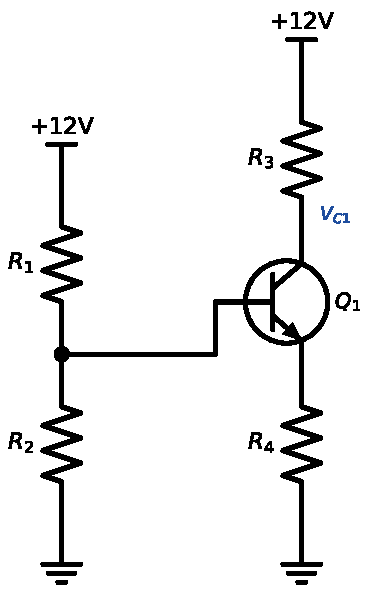
\includegraphics[width=\linewidth,height=6cm,keepaspectratio]{p01_circuit}\end{minipage}\hfill\begin{minipage}{0.38\linewidth}\begin{center}\small\renewcommand{\arraystretch}{1.35}
\begin{tabular}{ll}
\toprule
specification & value \\
\midrule
$I_{C1}$ & $1\,\mathrm{m}\mathrm{A}$ \\
$V_{C1}$ & $7\,\mathrm{V}$ \\
\bottomrule
\end{tabular}\end{center}
\end{minipage}
\end{probbox}

\begin{probbox}{Problem 4C.2 \hfill Easy}
Design the circuit below (find all resistor values) for the specifications in the table, such that every $I_B$ is negligible and $|V_{BE}| = 0.7 \pm 0.1$\,V changes every $I_C$ by less than 10\,\%. $\beta = 100$. Where the specifications leave a choice, use the smallest emitter-resistor voltage the $V_{BE}$ rule allows, divider current $I_{R2} = 1\,\mathrm{m}\mathrm{A}$.

\smallskip\noindent\begin{minipage}{0.6\linewidth}\centering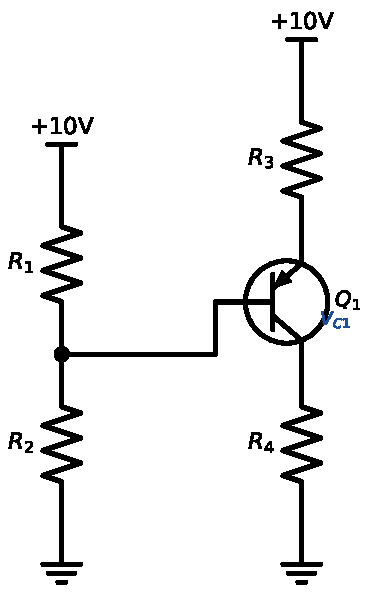
\includegraphics[width=\linewidth,height=6cm,keepaspectratio]{p02_circuit}\end{minipage}\hfill\begin{minipage}{0.38\linewidth}\begin{center}\small\renewcommand{\arraystretch}{1.35}
\begin{tabular}{ll}
\toprule
specification & value \\
\midrule
$I_{C1}$ & $2\,\mathrm{m}\mathrm{A}$ \\
$V_{C1}$ & $4\,\mathrm{V}$ \\
\bottomrule
\end{tabular}\end{center}
\end{minipage}
\end{probbox}

\begin{probbox}{Problem 4C.3 \hfill Easy}
Design the circuit below (find all resistor values) for the specifications in the table, such that every $I_B$ is negligible and $|V_{BE}| = 0.7 \pm 0.1$\,V changes every $I_C$ by less than 10\,\%. $\beta = 100$.

\smallskip\noindent\begin{minipage}{0.6\linewidth}\centering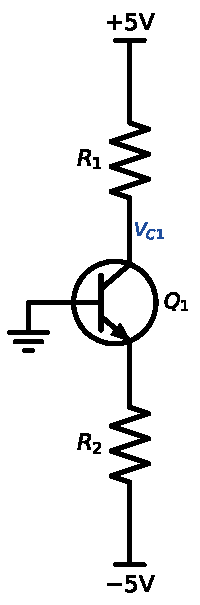
\includegraphics[width=\linewidth,height=6cm,keepaspectratio]{p03_circuit}\end{minipage}\hfill\begin{minipage}{0.38\linewidth}\begin{center}\small\renewcommand{\arraystretch}{1.35}
\begin{tabular}{ll}
\toprule
specification & value \\
\midrule
$I_{C1}$ & $1\,\mathrm{m}\mathrm{A}$ \\
$V_{C1}$ & $2\,\mathrm{V}$ \\
\bottomrule
\end{tabular}\end{center}
\end{minipage}
\end{probbox}

\begin{probbox}{Problem 4C.4 \hfill Easy}
Design the circuit below (find all resistor values) for the specifications in the table, such that every $I_B$ is negligible and $|V_{BE}| = 0.7 \pm 0.1$\,V changes every $I_C$ by less than 10\,\%. $\beta = 100$. Where the specifications leave a choice, use divider current $I_{R2} = 1\,\mathrm{m}\mathrm{A}$.

\smallskip\noindent\begin{minipage}{0.6\linewidth}\centering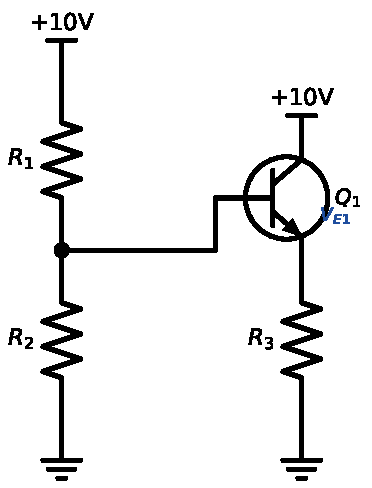
\includegraphics[width=\linewidth,height=6cm,keepaspectratio]{p04_circuit}\end{minipage}\hfill\begin{minipage}{0.38\linewidth}\begin{center}\small\renewcommand{\arraystretch}{1.35}
\begin{tabular}{ll}
\toprule
specification & value \\
\midrule
$I_{C1}$ & $5\,\mathrm{m}\mathrm{A}$ \\
$V_{E1}$ & $5\,\mathrm{V}$ \\
$|V_{CE}|$ (all transistors) & $\ge 1$\,V \\
\bottomrule
\end{tabular}\end{center}
\end{minipage}
\end{probbox}

\begin{probbox}{Problem 4C.5 \hfill Easy}
Design the circuit below (find all resistor values) for the specifications in the table, such that every $I_B$ is negligible and $|V_{BE}| = 0.7 \pm 0.1$\,V changes every $I_C$ by less than 10\,\%. $\beta = 100$.

\smallskip\noindent\begin{minipage}{0.6\linewidth}\centering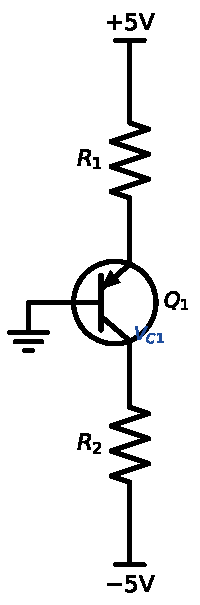
\includegraphics[width=\linewidth,height=6cm,keepaspectratio]{p05_circuit}\end{minipage}\hfill\begin{minipage}{0.38\linewidth}\begin{center}\small\renewcommand{\arraystretch}{1.35}
\begin{tabular}{ll}
\toprule
specification & value \\
\midrule
$I_{C1}$ & $2\,\mathrm{m}\mathrm{A}$ \\
$V_{C1}$ & $-1\,\mathrm{V}$ \\
\bottomrule
\end{tabular}\end{center}
\end{minipage}
\end{probbox}

\begin{probbox}{Problem 4C.6 \hfill Easy}
Design the circuit below (find all resistor values) for the specifications in the table, such that every $I_B$ is negligible and $|V_{BE}| = 0.7 \pm 0.1$\,V changes every $I_C$ by less than 10\,\%. $\beta = 100$. Where the specifications leave a choice, use the smallest emitter-resistor voltage the $V_{BE}$ rule allows, divider current $I_{R2} = 1\,\mathrm{m}\mathrm{A}$.

\smallskip\noindent\begin{minipage}{0.6\linewidth}\centering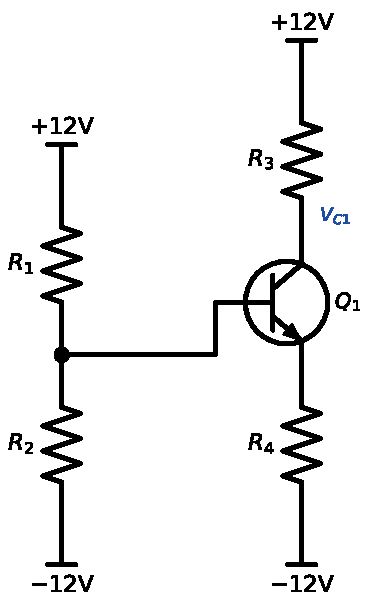
\includegraphics[width=\linewidth,height=6cm,keepaspectratio]{p06_circuit}\end{minipage}\hfill\begin{minipage}{0.38\linewidth}\begin{center}\small\renewcommand{\arraystretch}{1.35}
\begin{tabular}{ll}
\toprule
specification & value \\
\midrule
$I_{C1}$ & $2\,\mathrm{m}\mathrm{A}$ \\
$V_{C1}$ & $4\,\mathrm{V}$ \\
\bottomrule
\end{tabular}\end{center}
\end{minipage}
\end{probbox}

\subsection*{Medium problems}
\begin{probbox}{Problem 4C.7 \hfill Medium}
Design the circuit below (find all resistor values) for the specifications in the table, such that every $I_B$ is negligible and $|V_{BE}| = 0.7 \pm 0.1$\,V changes every $I_C$ by less than 10\,\%. $\beta = 100$. Where the specifications leave a choice, use the smallest emitter-resistor voltage the $V_{BE}$ rule allows, divider current $I_{R2} = 500\,\mu \mathrm{A}$.

\smallskip\noindent\begin{minipage}{0.6\linewidth}\centering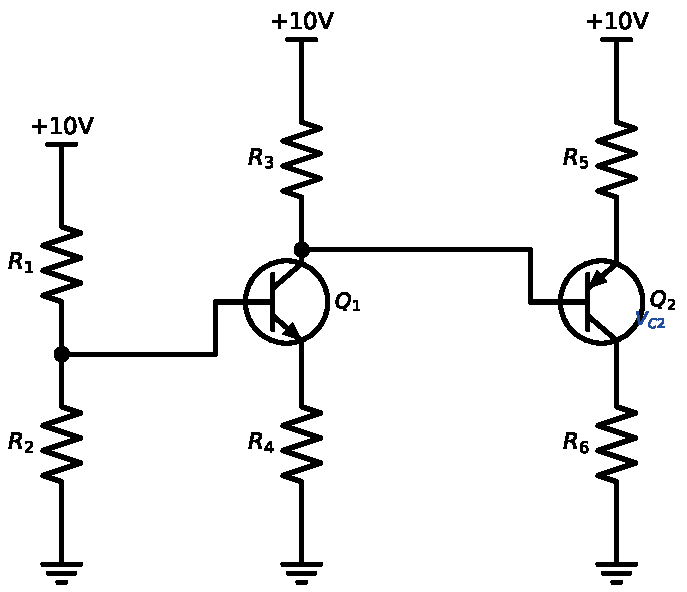
\includegraphics[width=\linewidth,height=6cm,keepaspectratio]{p07_circuit}\end{minipage}\hfill\begin{minipage}{0.38\linewidth}\begin{center}\small\renewcommand{\arraystretch}{1.35}
\begin{tabular}{ll}
\toprule
specification & value \\
\midrule
$I_{C1}$ & $1\,\mathrm{m}\mathrm{A}$ \\
$I_{C2}$ & $2\,\mathrm{m}\mathrm{A}$ \\
$V_{C2}$ & $4\,\mathrm{V}$ \\
$|V_{CE}|$ (all transistors) & $\ge 1$\,V \\
\bottomrule
\end{tabular}\end{center}
\end{minipage}
\end{probbox}

\begin{probbox}{Problem 4C.8 \hfill Medium}
Design the circuit below (find all resistor values) for the specifications in the table, such that every $I_B$ is negligible and $|V_{BE}| = 0.7 \pm 0.1$\,V changes every $I_C$ by less than 10\,\%. $\beta = 100$. Where the specifications leave a choice, use the smallest emitter-resistor voltage the $V_{BE}$ rule allows, divider current $I_{R2} = 500\,\mu \mathrm{A}$.

\smallskip\noindent\begin{minipage}{0.6\linewidth}\centering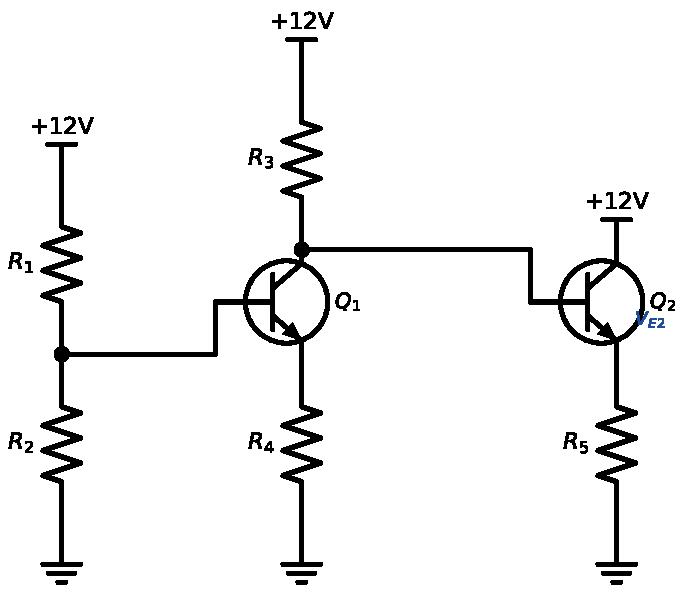
\includegraphics[width=\linewidth,height=6cm,keepaspectratio]{p08_circuit}\end{minipage}\hfill\begin{minipage}{0.38\linewidth}\begin{center}\small\renewcommand{\arraystretch}{1.35}
\begin{tabular}{ll}
\toprule
specification & value \\
\midrule
$I_{C1}$ & $1\,\mathrm{m}\mathrm{A}$ \\
$I_{C2}$ & $4\,\mathrm{m}\mathrm{A}$ \\
$V_{E2}$ & $6\,\mathrm{V}$ \\
$|V_{CE}|$ (all transistors) & $\ge 1$\,V \\
\bottomrule
\end{tabular}\end{center}
\end{minipage}
\end{probbox}

\begin{probbox}{Problem 4C.9 \hfill Medium}
Design the circuit below (find all resistor values) for the specifications in the table, such that every $I_B$ is negligible and $|V_{BE}| = 0.7 \pm 0.1$\,V changes every $I_C$ by less than 10\,\%. $\beta = 100$. Where the specifications leave a choice, use the smallest emitter-resistor voltage the $V_{BE}$ rule allows, divider current $I_{R2} = 500\,\mu \mathrm{A}$.

\smallskip\noindent\begin{minipage}{0.6\linewidth}\centering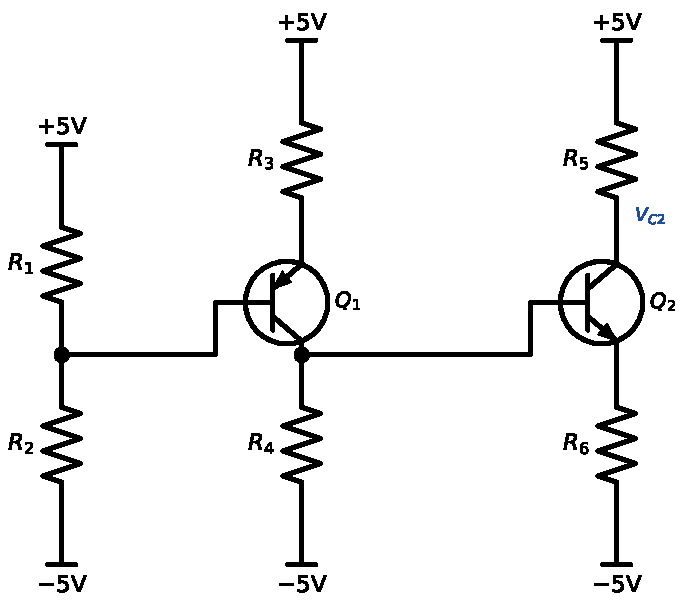
\includegraphics[width=\linewidth,height=6cm,keepaspectratio]{p09_circuit}\end{minipage}\hfill\begin{minipage}{0.38\linewidth}\begin{center}\small\renewcommand{\arraystretch}{1.35}
\begin{tabular}{ll}
\toprule
specification & value \\
\midrule
$I_{C1}$ & $1\,\mathrm{m}\mathrm{A}$ \\
$I_{C2}$ & $2\,\mathrm{m}\mathrm{A}$ \\
$V_{C2}$ & $1\,\mathrm{V}$ \\
$|V_{CE}|$ (all transistors) & $\ge 1$\,V \\
\bottomrule
\end{tabular}\end{center}
\end{minipage}
\end{probbox}

\begin{probbox}{Problem 4C.10 \hfill Medium}
Design the circuit below (find all resistor values) for the specifications in the table, such that every $I_B$ is negligible and $|V_{BE}| = 0.7 \pm 0.1$\,V changes every $I_C$ by less than 10\,\%. $\beta = 100$. Where the specifications leave a choice, use the smallest emitter-resistor voltage the $V_{BE}$ rule allows.

\smallskip\noindent\begin{minipage}{0.6\linewidth}\centering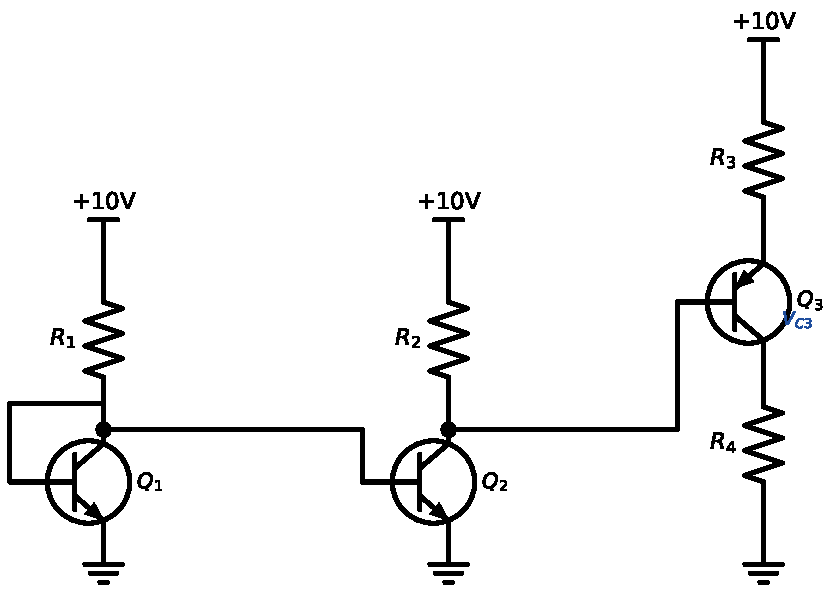
\includegraphics[width=\linewidth,height=6cm,keepaspectratio]{p10_circuit}\end{minipage}\hfill\begin{minipage}{0.38\linewidth}\begin{center}\small\renewcommand{\arraystretch}{1.35}
\begin{tabular}{ll}
\toprule
specification & value \\
\midrule
$I_{C1}$ & $1\,\mathrm{m}\mathrm{A}$ \\
$I_{C3}$ & $2\,\mathrm{m}\mathrm{A}$ \\
$V_{C3}$ & $3\,\mathrm{V}$ \\
$|V_{CE}|$ (all transistors) & $\ge 1$\,V \\
\bottomrule
\end{tabular}\end{center}
\end{minipage}
\end{probbox}

\begin{probbox}{Problem 4C.11 \hfill Medium}
Design the circuit below (find all resistor values) for the specifications in the table, such that every $I_B$ is negligible and $|V_{BE}| = 0.7 \pm 0.1$\,V changes every $I_C$ by less than 10\,\%. $\beta = 100$. Where the specifications leave a choice, use the smallest emitter-resistor voltage the $V_{BE}$ rule allows, divider current $I_{R2} = 500\,\mu \mathrm{A}$.

\smallskip\noindent\begin{minipage}{0.6\linewidth}\centering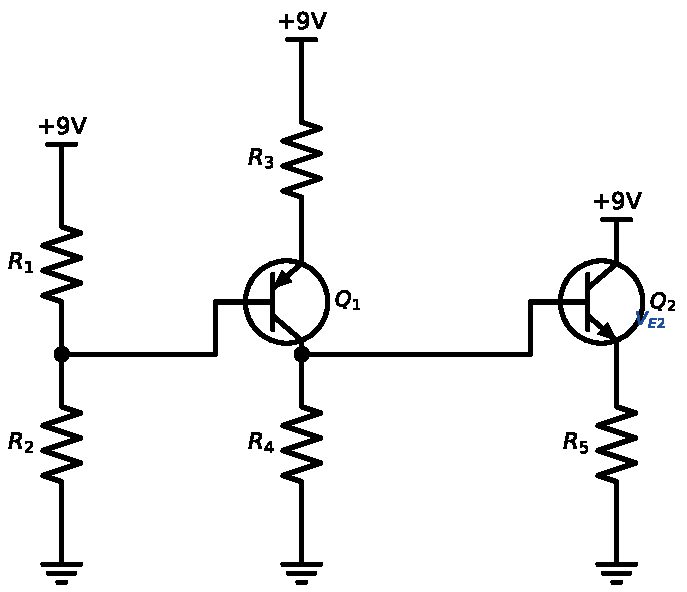
\includegraphics[width=\linewidth,height=6cm,keepaspectratio]{p11_circuit}\end{minipage}\hfill\begin{minipage}{0.38\linewidth}\begin{center}\small\renewcommand{\arraystretch}{1.35}
\begin{tabular}{ll}
\toprule
specification & value \\
\midrule
$I_{C1}$ & $1\,\mathrm{m}\mathrm{A}$ \\
$I_{C2}$ & $3\,\mathrm{m}\mathrm{A}$ \\
$V_{E2}$ & $3\,\mathrm{V}$ \\
$|V_{CE}|$ (all transistors) & $\ge 1$\,V \\
\bottomrule
\end{tabular}\end{center}
\end{minipage}
\end{probbox}

\begin{probbox}{Problem 4C.12 \hfill Medium}
Design the circuit below (find all resistor values) for the specifications in the table, such that every $I_B$ is negligible and $|V_{BE}| = 0.7 \pm 0.1$\,V changes every $I_C$ by less than 10\,\%. $\beta = 100$. Where the specifications leave a choice, use the smallest emitter-resistor voltage the $V_{BE}$ rule allows, divider current $I_{R2} = 500\,\mu \mathrm{A}$.

\smallskip\noindent\begin{minipage}{0.6\linewidth}\centering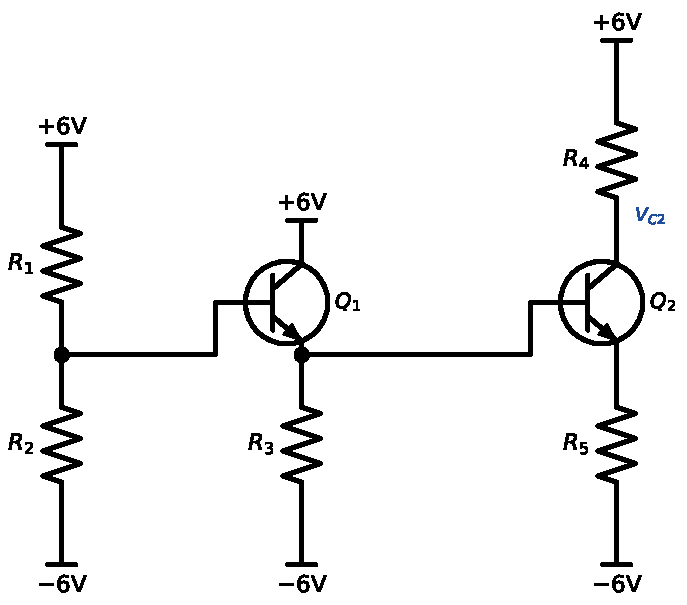
\includegraphics[width=\linewidth,height=6cm,keepaspectratio]{p12_circuit}\end{minipage}\hfill\begin{minipage}{0.38\linewidth}\begin{center}\small\renewcommand{\arraystretch}{1.35}
\begin{tabular}{ll}
\toprule
specification & value \\
\midrule
$I_{C1}$ & $1\,\mathrm{m}\mathrm{A}$ \\
$I_{C2}$ & $2\,\mathrm{m}\mathrm{A}$ \\
$V_{C2}$ & $2\,\mathrm{V}$ \\
$|V_{CE}|$ (all transistors) & $\ge 1$\,V \\
\bottomrule
\end{tabular}\end{center}
\end{minipage}
\end{probbox}

\subsection*{Hard problems}
\begin{probbox}{Problem 4C.13 \hfill Hard}
Design the circuit below (find all resistor values) for the specifications in the table, such that every $I_B$ is negligible and $|V_{BE}| = 0.7 \pm 0.1$\,V changes every $I_C$ by less than 10\,\%. $\beta = 100$. Where the specifications leave a choice, use the smallest emitter-resistor voltage the $V_{BE}$ rule allows. (This is Sample Problem 3 of the lecture.)

\smallskip\noindent\begin{minipage}{0.6\linewidth}\centering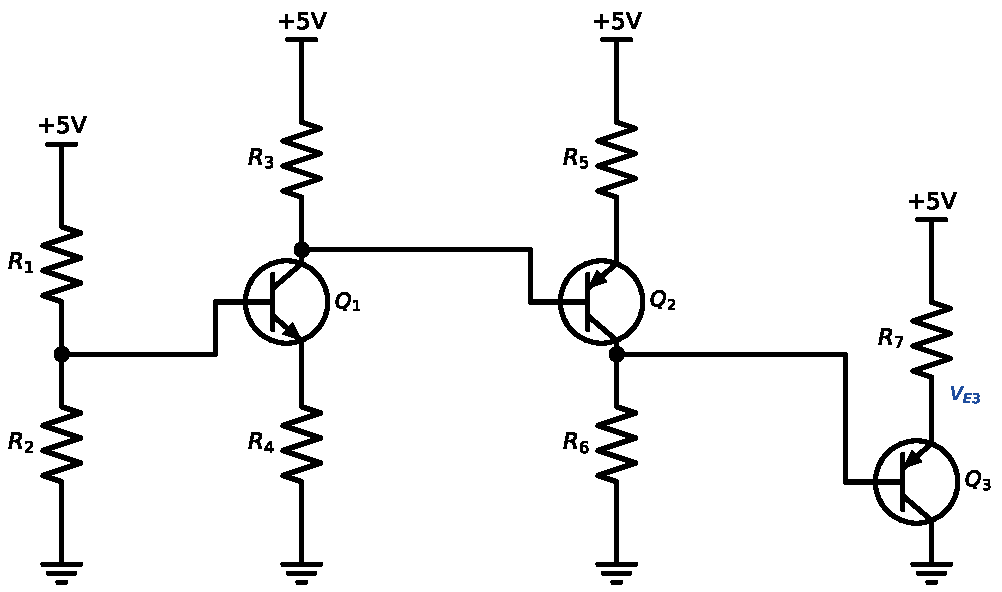
\includegraphics[width=\linewidth,height=6cm,keepaspectratio]{p13_circuit}\end{minipage}\hfill\begin{minipage}{0.38\linewidth}\begin{center}\small\renewcommand{\arraystretch}{1.35}
\begin{tabular}{ll}
\toprule
specification & value \\
\midrule
$I_{C1}$ & $2\,\mathrm{m}\mathrm{A}$ \\
$I_{C2}$ & $4\,\mathrm{m}\mathrm{A}$ \\
$I_{C3}$ & $6\,\mathrm{m}\mathrm{A}$ \\
$V_{E3}$ & $2.5\,\mathrm{V}$ \\
$|V_{CE}|$ (all transistors) & $\ge 1$\,V \\
$I_{dc}$ (supply current) & $\le 14\,\mathrm{m}\mathrm{A}$ \\
\bottomrule
\end{tabular}\end{center}
\end{minipage}
\end{probbox}

\begin{probbox}{Problem 4C.14 \hfill Hard}
Design the circuit below (find all resistor values) for the specifications in the table, such that every $I_B$ is negligible and $|V_{BE}| = 0.7 \pm 0.1$\,V changes every $I_C$ by less than 10\,\%. $\beta = 100$. Where the specifications leave a choice, use the smallest emitter-resistor voltage the $V_{BE}$ rule allows.

\smallskip\noindent\begin{minipage}{0.6\linewidth}\centering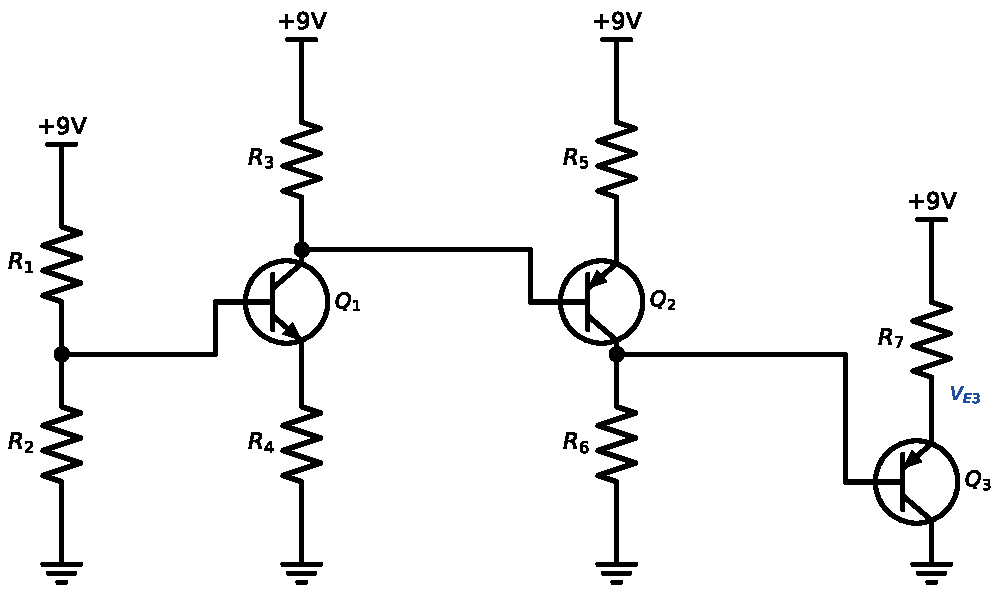
\includegraphics[width=\linewidth,height=6cm,keepaspectratio]{p14_circuit}\end{minipage}\hfill\begin{minipage}{0.38\linewidth}\begin{center}\small\renewcommand{\arraystretch}{1.35}
\begin{tabular}{ll}
\toprule
specification & value \\
\midrule
$I_{C1}$ & $1\,\mathrm{m}\mathrm{A}$ \\
$I_{C2}$ & $2\,\mathrm{m}\mathrm{A}$ \\
$I_{C3}$ & $5\,\mathrm{m}\mathrm{A}$ \\
$V_{E3}$ & $5\,\mathrm{V}$ \\
$|V_{CE}|$ (all transistors) & $\ge 1$\,V \\
$I_{dc}$ (supply current) & $\le 9\,\mathrm{m}\mathrm{A}$ \\
\bottomrule
\end{tabular}\end{center}
\end{minipage}
\end{probbox}

\begin{probbox}{Problem 4C.15 \hfill Hard}
Design the circuit below (find all resistor values) for the specifications in the table, such that every $I_B$ is negligible and $|V_{BE}| = 0.7 \pm 0.1$\,V changes every $I_C$ by less than 10\,\%. $\beta = 100$. Where the specifications leave a choice, use the smallest emitter-resistor voltage the $V_{BE}$ rule allows, $V_{R5} = 2$\,V, $V_{R8} = 2$\,V, divider current $I_{R2} = 500\,\mu \mathrm{A}$.

\smallskip\noindent\begin{minipage}{0.6\linewidth}\centering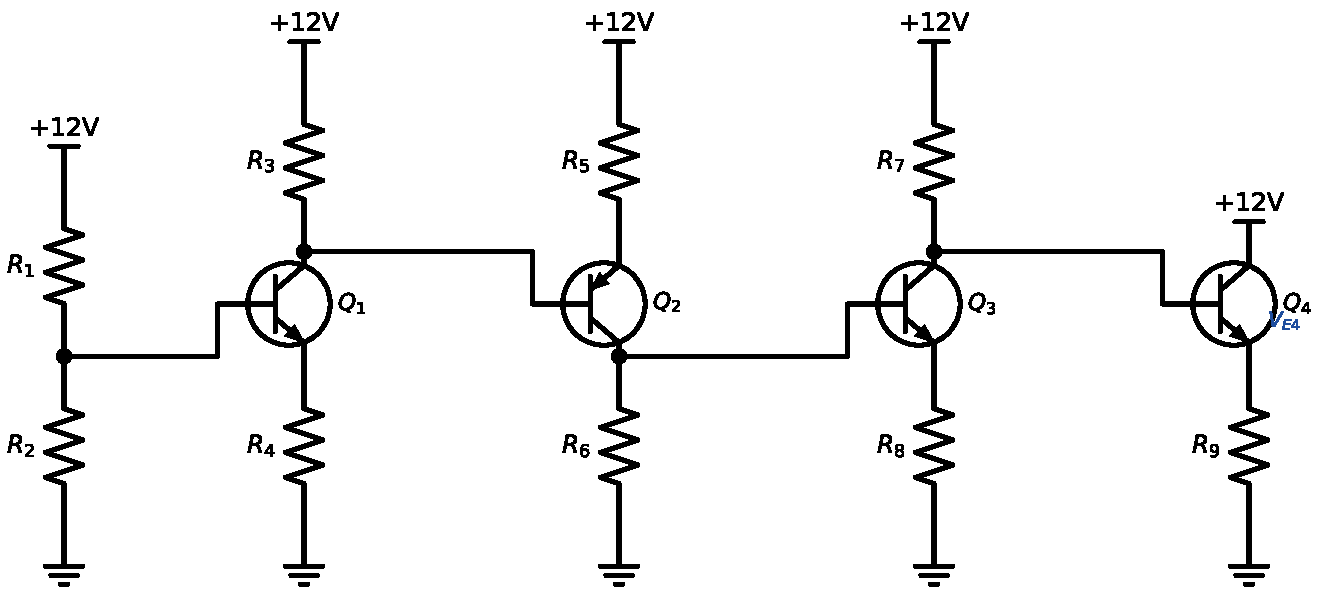
\includegraphics[width=\linewidth,height=6cm,keepaspectratio]{p15_circuit}\end{minipage}\hfill\begin{minipage}{0.38\linewidth}\begin{center}\small\renewcommand{\arraystretch}{1.35}
\begin{tabular}{ll}
\toprule
specification & value \\
\midrule
$I_{C1}$ & $1\,\mathrm{m}\mathrm{A}$ \\
$I_{C2}$ & $2\,\mathrm{m}\mathrm{A}$ \\
$I_{C3}$ & $2\,\mathrm{m}\mathrm{A}$ \\
$I_{C4}$ & $5\,\mathrm{m}\mathrm{A}$ \\
$V_{E4}$ & $6\,\mathrm{V}$ \\
$|V_{CE}|$ (all transistors) & $\ge 1$\,V \\
\bottomrule
\end{tabular}\end{center}
\end{minipage}
\end{probbox}

\begin{probbox}{Problem 4C.16 \hfill Hard}
Design the circuit below (find all resistor values) for the specifications in the table, such that every $I_B$ is negligible and $|V_{BE}| = 0.7 \pm 0.1$\,V changes every $I_C$ by less than 10\,\%. $\beta = 100$.

\smallskip\noindent\begin{minipage}{0.6\linewidth}\centering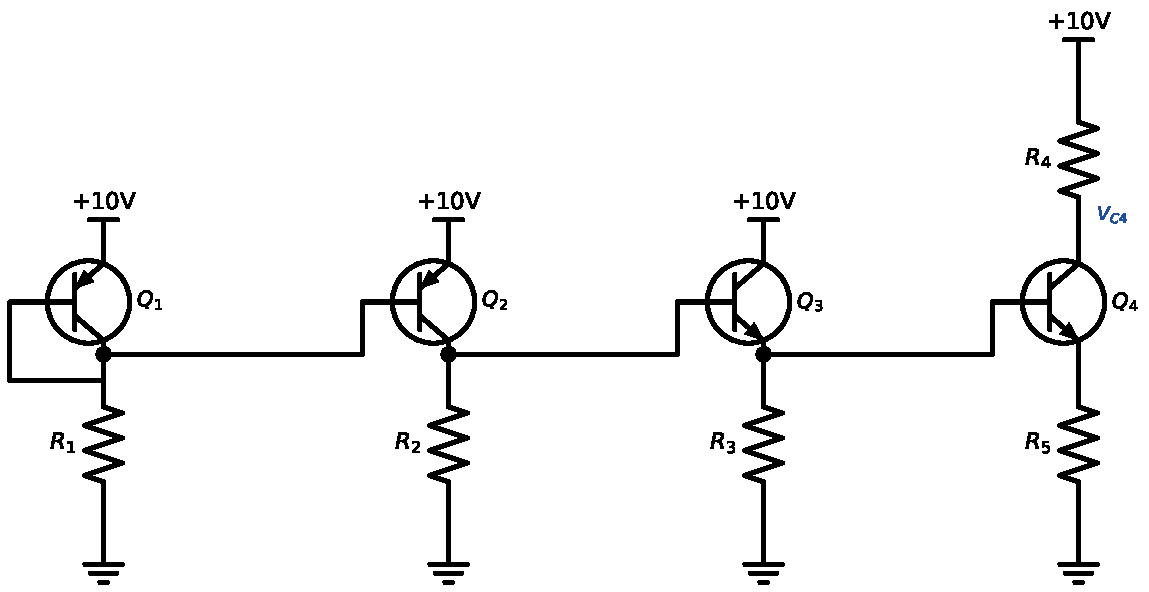
\includegraphics[width=\linewidth,height=6cm,keepaspectratio]{p16_circuit}\end{minipage}\hfill\begin{minipage}{0.38\linewidth}\begin{center}\small\renewcommand{\arraystretch}{1.35}
\begin{tabular}{ll}
\toprule
specification & value \\
\midrule
$I_{C1}$ & $2\,\mathrm{m}\mathrm{A}$ \\
$I_{C3}$ & $4\,\mathrm{m}\mathrm{A}$ \\
$I_{C4}$ & $1\,\mathrm{m}\mathrm{A}$ \\
$V_{E3}$ & $4\,\mathrm{V}$ \\
$V_{C4}$ & $7\,\mathrm{V}$ \\
$|V_{CE}|$ (all transistors) & $\ge 1$\,V \\
$I_{dc}$ (supply current) & $\le 10\,\mathrm{m}\mathrm{A}$ \\
\bottomrule
\end{tabular}\end{center}
\end{minipage}
\end{probbox}

\begin{probbox}{Problem 4C.17 \hfill Hard}
Design the circuit below (find all resistor values) for the specifications in the table, such that every $I_B$ is negligible and $|V_{BE}| = 0.7 \pm 0.1$\,V changes every $I_C$ by less than 10\,\%. $\beta = 100$. Where the specifications leave a choice, use the smallest emitter-resistor voltage the $V_{BE}$ rule allows.

\smallskip\noindent\begin{minipage}{0.6\linewidth}\centering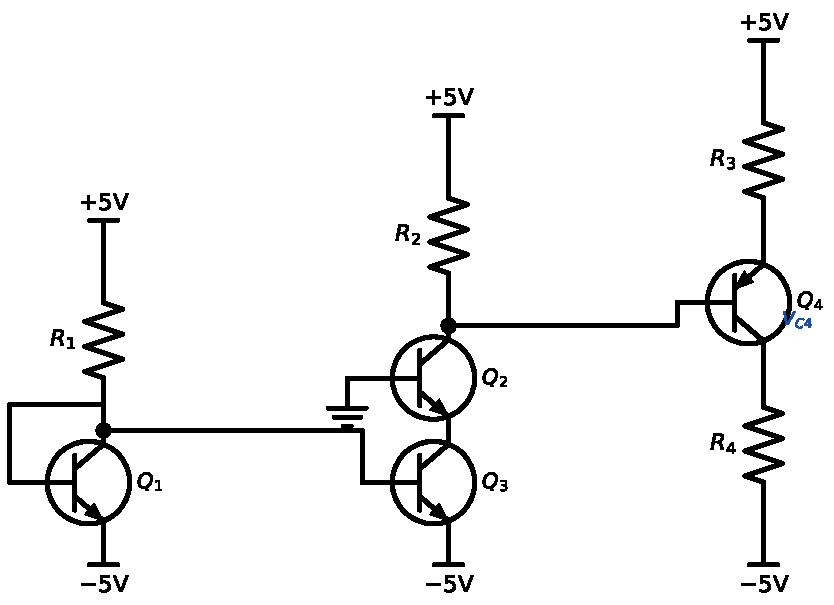
\includegraphics[width=\linewidth,height=6cm,keepaspectratio]{p17_circuit}\end{minipage}\hfill\begin{minipage}{0.38\linewidth}\begin{center}\small\renewcommand{\arraystretch}{1.35}
\begin{tabular}{ll}
\toprule
specification & value \\
\midrule
$I_{C1}$ & $1\,\mathrm{m}\mathrm{A}$ \\
$I_{C4}$ & $2\,\mathrm{m}\mathrm{A}$ \\
$V_{C4}$ & $-1\,\mathrm{V}$ \\
$|V_{CE}|$ (all transistors) & $\ge 1$\,V \\
\bottomrule
\end{tabular}\end{center}
\end{minipage}
\end{probbox}

\begin{probbox}{Problem 4C.18 \hfill Hard}
Design the circuit below (find all resistor values) for the specifications in the table, such that every $I_B$ is negligible and $|V_{BE}| = 0.7 \pm 0.1$\,V changes every $I_C$ by less than 10\,\%. $\beta = 100$. Where the specifications leave a choice, use the smallest emitter-resistor voltage the $V_{BE}$ rule allows.

\smallskip\noindent\begin{minipage}{0.6\linewidth}\centering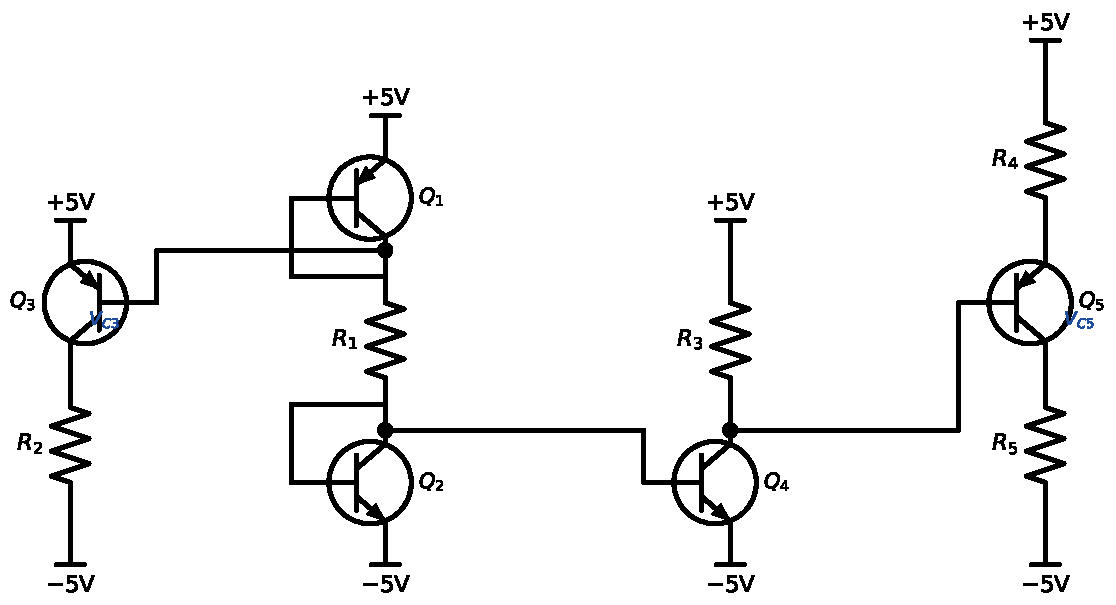
\includegraphics[width=\linewidth,height=6cm,keepaspectratio]{p18_circuit}\end{minipage}\hfill\begin{minipage}{0.38\linewidth}\begin{center}\small\renewcommand{\arraystretch}{1.35}
\begin{tabular}{ll}
\toprule
specification & value \\
\midrule
$I_{C1}$ & $1\,\mathrm{m}\mathrm{A}$ \\
$I_{C5}$ & $2\,\mathrm{m}\mathrm{A}$ \\
$V_{C3}$ & $2\,\mathrm{V}$ \\
$V_{C5}$ & $-2\,\mathrm{V}$ \\
$|V_{CE}|$ (all transistors) & $\ge 1$\,V \\
\bottomrule
\end{tabular}\end{center}
\end{minipage}
\end{probbox}

\newpage
\section*{Solutions}
Every solution follows the steps of the Lecture-4 pipeline card.
\subsection*{Solution 4C.1 \hfill Easy}
\begin{center}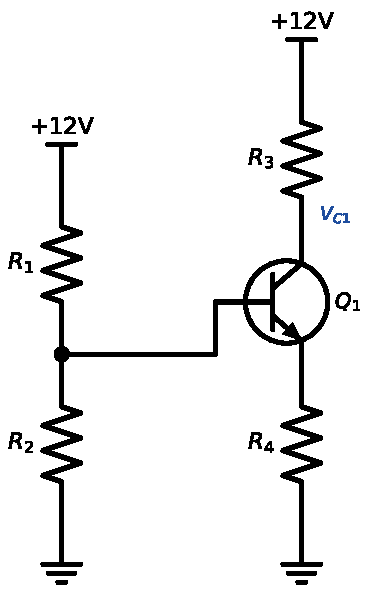
\includegraphics[width=0.9\linewidth,height=6cm,keepaspectratio]{p01_circuit}\end{center}
\solstep{1}{Rules}With $I_B\approx0$ and every transistor active ($|V_{BE}|=0.7$\,V, $I_C\approx I_E$), a resistor is known as soon as the voltages at both of its ends and the current through it are known: $R = \Delta V / I$. The specifications give the currents and some node voltages; the remaining freedom is removed with two rules:\begin{itemize}[leftmargin=*,itemsep=1pt]
\item $V_{BE}$-insensitive: the voltage across the resistor that sets an emitter current must be at least $1$\,V (then $\pm0.1$\,V of $V_{BE}$ changes $I_C$ by at most $10\,\%$);
\item $\beta$-insensitive: a divider current must be much larger ($\ge 10\times$) than the base current it feeds, and a collector current that drives a base must be much larger than that base current.
\end{itemize}
Work from the nodes that are already fixed towards the unknown ones.
\solstep{2}{Design, node by node}\begin{enumerate}[leftmargin=*,itemsep=3pt]
\item $V_{BE}$-insensitivity: a $0.1$\,V change of $V_{BE}$ changes the voltage across $R_{4}$ by $0.1$\,V, so $\frac{\Delta I_C}{I_C} = \frac{0.1}{V_{R4}} \le 10\%$ needs $V_{R4} \ge 1$\,V. Choose the smallest value, $V_{R4} = 1$\,V: $V_{E1} = 0 + V_{R4} = 0 + 1 = 1\,\mathrm{V}$.
\item The divider current must be much larger than the base current it feeds ($I_{B1} = 10\,\mu \mathrm{A}$). Choose $I_{R2} = 500\,\mu \mathrm{A}$ (50 times larger).
\item $Q_{1}$ is active: $V_{B1} = V_{E1} + 0.7 = 1.7\,\mathrm{V}$.
\item With $I_B\approx0$ the only current through $R_{1}$ is $I_{R2}$: $I_{R1} = I_{R2} = 500\,\mu \mathrm{A}$.
\item $\displaystyle R_{1} = \frac{12 - V_{B1}}{I_{R2}} = \frac{12 - 1.7}{500\,\mu \mathrm{A}} = \mathbf{20.6\,\mathrm{k}\Omega}$
\item $\displaystyle R_{2} = \frac{V_{B1} - 0}{I_{R2}} = \frac{1.7 - 0}{500\,\mu \mathrm{A}} = \mathbf{3.4\,\mathrm{k}\Omega}$
\item With $I_B\approx0$ the only current through $R_{3}$ is $I_{C1}$: $I_{R3} = I_{C1} = 1\,\mathrm{m}\mathrm{A}$.
\item $\displaystyle R_{3} = \frac{12 - V_{C1}}{I_{C1}} = \frac{12 - 7}{1\,\mathrm{m}\mathrm{A}} = \mathbf{5\,\mathrm{k}\Omega}$
\item With $I_B\approx0$ the only current through $R_{4}$ is $I_{E1}$: $I_{R4} = I_{E1} = 1\,\mathrm{m}\mathrm{A}$ ($I_C\approx I_E$).
\item $\displaystyle R_{4} = \frac{V_{E1} - 0}{I_{E1}} = \frac{1 - 0}{1\,\mathrm{m}\mathrm{A}} = \mathbf{1\,\mathrm{k}\Omega}$
\end{enumerate}

\solstep{3}{Designed circuit}\begin{center}\renewcommand{\arraystretch}{1.35}
\begin{tabular}{cc}
\toprule
resistor & value \\
\midrule
$R_{1}$ & $20.6\,\mathrm{k}\Omega$ \\
$R_{2}$ & $3.4\,\mathrm{k}\Omega$ \\
$R_{3}$ & $5\,\mathrm{k}\Omega$ \\
$R_{4}$ & $1\,\mathrm{k}\Omega$ \\
\bottomrule
\end{tabular}\end{center}
\begin{center}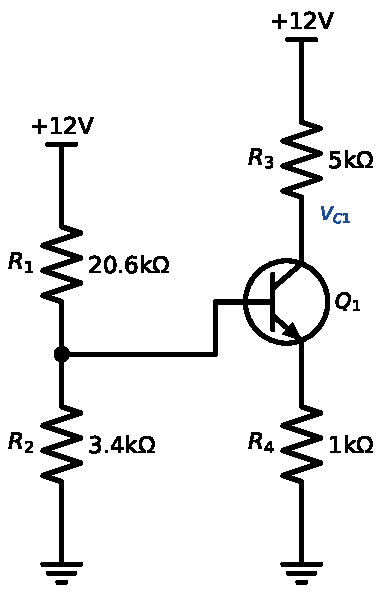
\includegraphics[width=0.85\linewidth,height=6cm,keepaspectratio]{p01_designed}\end{center}

\solstep{4}{Check the design}\begin{itemize}[leftmargin=*,itemsep=2pt]
\item $I_{B1} = \frac{I_{C1}}{\beta} = 10\,\mu \mathrm{A}$ $\ll$ the $500\,\mu \mathrm{A}$ flowing in the base network \checkmark
\item $V_{CE1} = V_{C1} - V_{E1} = 7 - 1 = 6\,\mathrm{V} \ge 0.2$\,V \checkmark
\end{itemize}
Finally the designed circuit is solved exactly ($\beta=100$, base currents included), once with $|V_{BE}|=0.7$\,V and once with each transistor's $|V_{BE}|$ changed to $0.6$ and $0.8$\,V:\begin{center}\renewcommand{\arraystretch}{1.35}
\begin{tabular}{cccccc}
\toprule
 & target $I_C$ & exact $I_C$ & $|V_{BE}|=0.6$ & $|V_{BE}|=0.8$ & max change \\
\midrule
$Q_{1}$ & $1\,\mathrm{m}\mathrm{A}$ & $962\,\mu \mathrm{A}$ & $1.06\,\mathrm{m}\mathrm{A}$ & $866\,\mu \mathrm{A}$ & $9.6\,\%$ \\
\bottomrule
\end{tabular}\end{center}
A $\pm0.1$\,V change of $V_{BE}$ moves no current by more than about $10\,\%$ of its design value ($V_{BE}$-insensitive), and the exact currents are close to the targets ($I_B$ negligible).
\begin{ansbox}
$R_{1} = 20.6\,\mathrm{k}\Omega$,\quad $R_{2} = 3.4\,\mathrm{k}\Omega$,\quad $R_{3} = 5\,\mathrm{k}\Omega$,\quad $R_{4} = 1\,\mathrm{k}\Omega$
\end{ansbox}

\newpage
\subsection*{Solution 4C.2 \hfill Easy}
\begin{center}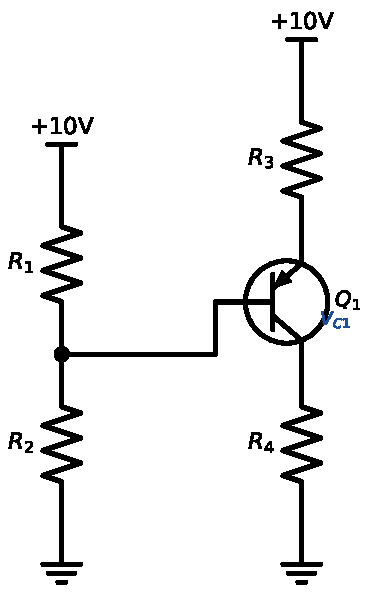
\includegraphics[width=0.9\linewidth,height=6cm,keepaspectratio]{p02_circuit}\end{center}
\solstep{1}{Rules}With $I_B\approx0$ and every transistor active ($|V_{BE}|=0.7$\,V, $I_C\approx I_E$), a resistor is known as soon as the voltages at both of its ends and the current through it are known: $R = \Delta V / I$. The specifications give the currents and some node voltages; the remaining freedom is removed with two rules:\begin{itemize}[leftmargin=*,itemsep=1pt]
\item $V_{BE}$-insensitive: the voltage across the resistor that sets an emitter current must be at least $1$\,V (then $\pm0.1$\,V of $V_{BE}$ changes $I_C$ by at most $10\,\%$);
\item $\beta$-insensitive: a divider current must be much larger ($\ge 10\times$) than the base current it feeds, and a collector current that drives a base must be much larger than that base current.
\end{itemize}
Work from the nodes that are already fixed towards the unknown ones.
\solstep{2}{Design, node by node}\begin{enumerate}[leftmargin=*,itemsep=3pt]
\item $V_{BE}$-insensitivity: a $0.1$\,V change of $V_{BE}$ changes the voltage across $R_{3}$ by $0.1$\,V, so $\frac{\Delta I_C}{I_C} = \frac{0.1}{V_{R3}} \le 10\%$ needs $V_{R3} \ge 1$\,V. Choose the smallest value, $V_{R3} = 1$\,V: $V_{E1} = 10 - V_{R3} = 10 - 1 = 9\,\mathrm{V}$.
\item The divider current must be much larger than the base current it feeds ($I_{B1} = 20\,\mu \mathrm{A}$). Choose $I_{R2} = 1\,\mathrm{m}\mathrm{A}$ (50 times larger).
\item $Q_{1}$ is active: $V_{B1} = V_{E1} - 0.7 = 8.3\,\mathrm{V}$.
\item With $I_B\approx0$ the only current through $R_{1}$ is $I_{R2}$: $I_{R1} = I_{R2} = 1\,\mathrm{m}\mathrm{A}$.
\item $\displaystyle R_{1} = \frac{10 - V_{B1}}{I_{R2}} = \frac{10 - 8.3}{1\,\mathrm{m}\mathrm{A}} = \mathbf{1.7\,\mathrm{k}\Omega}$
\item $\displaystyle R_{2} = \frac{V_{B1} - 0}{I_{R2}} = \frac{8.3 - 0}{1\,\mathrm{m}\mathrm{A}} = \mathbf{8.3\,\mathrm{k}\Omega}$
\item With $I_B\approx0$ the only current through $R_{3}$ is $I_{E1}$: $I_{R3} = I_{E1} = 2\,\mathrm{m}\mathrm{A}$ ($I_C\approx I_E$).
\item $\displaystyle R_{3} = \frac{10 - V_{E1}}{I_{E1}} = \frac{10 - 9}{2\,\mathrm{m}\mathrm{A}} = \mathbf{500\,\Omega}$
\item With $I_B\approx0$ the only current through $R_{4}$ is $I_{C1}$: $I_{R4} = I_{C1} = 2\,\mathrm{m}\mathrm{A}$.
\item $\displaystyle R_{4} = \frac{V_{C1} - 0}{I_{C1}} = \frac{4 - 0}{2\,\mathrm{m}\mathrm{A}} = \mathbf{2\,\mathrm{k}\Omega}$
\end{enumerate}

\solstep{3}{Designed circuit}\begin{center}\renewcommand{\arraystretch}{1.35}
\begin{tabular}{cc}
\toprule
resistor & value \\
\midrule
$R_{1}$ & $1.7\,\mathrm{k}\Omega$ \\
$R_{2}$ & $8.3\,\mathrm{k}\Omega$ \\
$R_{3}$ & $500\,\Omega$ \\
$R_{4}$ & $2\,\mathrm{k}\Omega$ \\
\bottomrule
\end{tabular}\end{center}
\begin{center}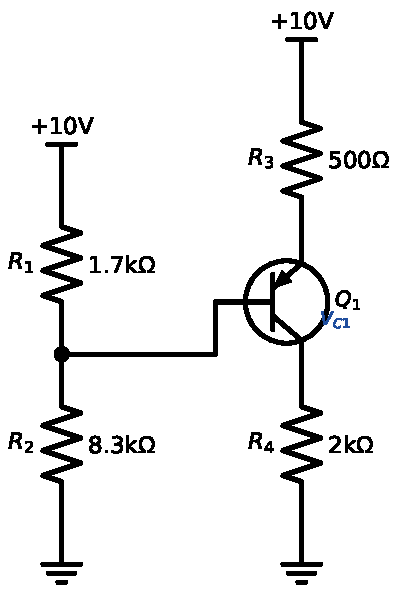
\includegraphics[width=0.85\linewidth,height=6cm,keepaspectratio]{p02_designed}\end{center}

\solstep{4}{Check the design}\begin{itemize}[leftmargin=*,itemsep=2pt]
\item $I_{B1} = \frac{I_{C1}}{\beta} = 20\,\mu \mathrm{A}$ $\ll$ the $1\,\mathrm{m}\mathrm{A}$ flowing in the base network \checkmark
\item $V_{EC1} = V_{E1} - V_{C1} = 9 - 4 = 5\,\mathrm{V} \ge 0.2$\,V \checkmark
\end{itemize}
Finally the designed circuit is solved exactly ($\beta=100$, base currents included), once with $|V_{BE}|=0.7$\,V and once with each transistor's $|V_{BE}|$ changed to $0.6$ and $0.8$\,V:\begin{center}\renewcommand{\arraystretch}{1.35}
\begin{tabular}{cccccc}
\toprule
 & target $I_C$ & exact $I_C$ & $|V_{BE}|=0.6$ & $|V_{BE}|=0.8$ & max change \\
\midrule
$Q_{1}$ & $2\,\mathrm{m}\mathrm{A}$ & $1.93\,\mathrm{m}\mathrm{A}$ & $2.12\,\mathrm{m}\mathrm{A}$ & $1.73\,\mathrm{m}\mathrm{A}$ & $9.6\,\%$ \\
\bottomrule
\end{tabular}\end{center}
A $\pm0.1$\,V change of $V_{BE}$ moves no current by more than about $10\,\%$ of its design value ($V_{BE}$-insensitive), and the exact currents are close to the targets ($I_B$ negligible).
\begin{ansbox}
$R_{1} = 1.7\,\mathrm{k}\Omega$,\quad $R_{2} = 8.3\,\mathrm{k}\Omega$,\quad $R_{3} = 500\,\Omega$,\quad $R_{4} = 2\,\mathrm{k}\Omega$
\end{ansbox}

\newpage
\subsection*{Solution 4C.3 \hfill Easy}
\begin{center}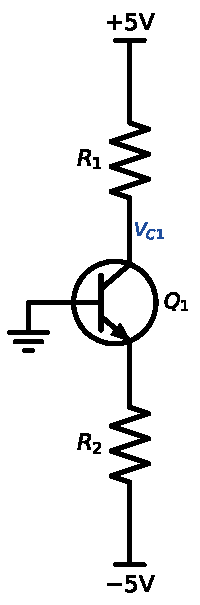
\includegraphics[width=0.9\linewidth,height=6cm,keepaspectratio]{p03_circuit}\end{center}
\solstep{1}{Rules}With $I_B\approx0$ and every transistor active ($|V_{BE}|=0.7$\,V, $I_C\approx I_E$), a resistor is known as soon as the voltages at both of its ends and the current through it are known: $R = \Delta V / I$. The specifications give the currents and some node voltages; the remaining freedom is removed with two rules:\begin{itemize}[leftmargin=*,itemsep=1pt]
\item $V_{BE}$-insensitive: the voltage across the resistor that sets an emitter current must be at least $1$\,V (then $\pm0.1$\,V of $V_{BE}$ changes $I_C$ by at most $10\,\%$);
\item $\beta$-insensitive: a divider current must be much larger ($\ge 10\times$) than the base current it feeds, and a collector current that drives a base must be much larger than that base current.
\end{itemize}
Work from the nodes that are already fixed towards the unknown ones.
\solstep{2}{Design, node by node}\begin{enumerate}[leftmargin=*,itemsep=3pt]
\item $Q_{1}$ is active: $V_{E1} = 0 - 0.7 = -0.7\,\mathrm{V}$.
\item With $I_B\approx0$ the only current through $R_{1}$ is $I_{C1}$: $I_{R1} = I_{C1} = 1\,\mathrm{m}\mathrm{A}$.
\item $\displaystyle R_{1} = \frac{5 - V_{C1}}{I_{C1}} = \frac{5 - 2}{1\,\mathrm{m}\mathrm{A}} = \mathbf{3\,\mathrm{k}\Omega}$
\item With $I_B\approx0$ the only current through $R_{2}$ is $I_{E1}$: $I_{R2} = I_{E1} = 1\,\mathrm{m}\mathrm{A}$ ($I_C\approx I_E$).
\item $\displaystyle R_{2} = \frac{V_{E1} - (-5)}{I_{E1}} = \frac{-0.7 - (-5)}{1\,\mathrm{m}\mathrm{A}} = \mathbf{4.3\,\mathrm{k}\Omega}$
\end{enumerate}

\solstep{3}{Designed circuit}\begin{center}\renewcommand{\arraystretch}{1.35}
\begin{tabular}{cc}
\toprule
resistor & value \\
\midrule
$R_{1}$ & $3\,\mathrm{k}\Omega$ \\
$R_{2}$ & $4.3\,\mathrm{k}\Omega$ \\
\bottomrule
\end{tabular}\end{center}
\begin{center}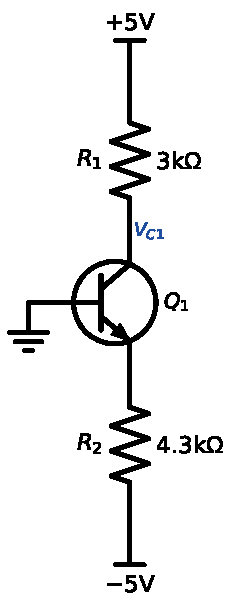
\includegraphics[width=0.85\linewidth,height=6cm,keepaspectratio]{p03_designed}\end{center}

\solstep{4}{Check the design}\begin{itemize}[leftmargin=*,itemsep=2pt]
\item $V_{CE1} = V_{C1} - V_{E1} = 2 - (-0.7) = 2.7\,\mathrm{V} \ge 0.2$\,V \checkmark
\end{itemize}
Finally the designed circuit is solved exactly ($\beta=100$, base currents included), once with $|V_{BE}|=0.7$\,V and once with each transistor's $|V_{BE}|$ changed to $0.6$ and $0.8$\,V:\begin{center}\renewcommand{\arraystretch}{1.35}
\begin{tabular}{cccccc}
\toprule
 & target $I_C$ & exact $I_C$ & $|V_{BE}|=0.6$ & $|V_{BE}|=0.8$ & max change \\
\midrule
$Q_{1}$ & $1\,\mathrm{m}\mathrm{A}$ & $990\,\mu \mathrm{A}$ & $1.01\,\mathrm{m}\mathrm{A}$ & $967\,\mu \mathrm{A}$ & $2.3\,\%$ \\
\bottomrule
\end{tabular}\end{center}
A $\pm0.1$\,V change of $V_{BE}$ moves no current by more than about $10\,\%$ of its design value ($V_{BE}$-insensitive), and the exact currents are close to the targets ($I_B$ negligible).
\begin{ansbox}
$R_{1} = 3\,\mathrm{k}\Omega$,\quad $R_{2} = 4.3\,\mathrm{k}\Omega$
\end{ansbox}

\newpage
\subsection*{Solution 4C.4 \hfill Easy}
\begin{center}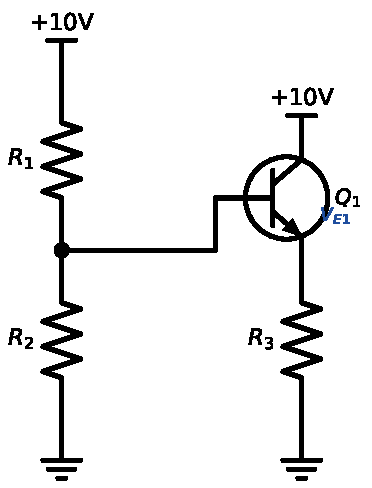
\includegraphics[width=0.9\linewidth,height=6cm,keepaspectratio]{p04_circuit}\end{center}
\solstep{1}{Rules}With $I_B\approx0$ and every transistor active ($|V_{BE}|=0.7$\,V, $I_C\approx I_E$), a resistor is known as soon as the voltages at both of its ends and the current through it are known: $R = \Delta V / I$. The specifications give the currents and some node voltages; the remaining freedom is removed with two rules:\begin{itemize}[leftmargin=*,itemsep=1pt]
\item $V_{BE}$-insensitive: the voltage across the resistor that sets an emitter current must be at least $1$\,V (then $\pm0.1$\,V of $V_{BE}$ changes $I_C$ by at most $10\,\%$);
\item $\beta$-insensitive: a divider current must be much larger ($\ge 10\times$) than the base current it feeds, and a collector current that drives a base must be much larger than that base current.
\end{itemize}
Work from the nodes that are already fixed towards the unknown ones.
\solstep{2}{Design, node by node}\begin{enumerate}[leftmargin=*,itemsep=3pt]
\item The divider current must be much larger than the base current it feeds ($I_{B1} = 50\,\mu \mathrm{A}$). Choose $I_{R2} = 1\,\mathrm{m}\mathrm{A}$ (20 times larger).
\item $Q_{1}$ is active: $V_{B1} = V_{E1} + 0.7 = 5.7\,\mathrm{V}$.
\item With $I_B\approx0$ the only current through $R_{1}$ is $I_{R2}$: $I_{R1} = I_{R2} = 1\,\mathrm{m}\mathrm{A}$.
\item $\displaystyle R_{1} = \frac{10 - V_{B1}}{I_{R2}} = \frac{10 - 5.7}{1\,\mathrm{m}\mathrm{A}} = \mathbf{4.3\,\mathrm{k}\Omega}$
\item $\displaystyle R_{2} = \frac{V_{B1} - 0}{I_{R2}} = \frac{5.7 - 0}{1\,\mathrm{m}\mathrm{A}} = \mathbf{5.7\,\mathrm{k}\Omega}$
\item With $I_B\approx0$ the only current through $R_{3}$ is $I_{E1}$: $I_{R3} = I_{E1} = 5\,\mathrm{m}\mathrm{A}$ ($I_C\approx I_E$).
\item $\displaystyle R_{3} = \frac{V_{E1} - 0}{I_{E1}} = \frac{5 - 0}{5\,\mathrm{m}\mathrm{A}} = \mathbf{1\,\mathrm{k}\Omega}$
\end{enumerate}

\solstep{3}{Designed circuit}\begin{center}\renewcommand{\arraystretch}{1.35}
\begin{tabular}{cc}
\toprule
resistor & value \\
\midrule
$R_{1}$ & $4.3\,\mathrm{k}\Omega$ \\
$R_{2}$ & $5.7\,\mathrm{k}\Omega$ \\
$R_{3}$ & $1\,\mathrm{k}\Omega$ \\
\bottomrule
\end{tabular}\end{center}
\begin{center}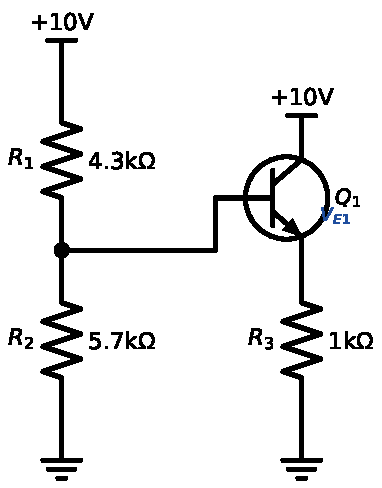
\includegraphics[width=0.85\linewidth,height=6cm,keepaspectratio]{p04_designed}\end{center}

\solstep{4}{Check the design}\begin{itemize}[leftmargin=*,itemsep=2pt]
\item $I_{B1} = \frac{I_{C1}}{\beta} = 50\,\mu \mathrm{A}$ $\ll$ the $1\,\mathrm{m}\mathrm{A}$ flowing in the base network \checkmark
\item $V_{CE1} = 10 - V_{E1} = 10 - 5 = 5\,\mathrm{V} \ge 1$\,V \checkmark
\end{itemize}
Finally the designed circuit is solved exactly ($\beta=100$, base currents included), once with $|V_{BE}|=0.7$\,V and once with each transistor's $|V_{BE}|$ changed to $0.6$ and $0.8$\,V:\begin{center}\renewcommand{\arraystretch}{1.35}
\begin{tabular}{cccccc}
\toprule
 & target $I_C$ & exact $I_C$ & $|V_{BE}|=0.6$ & $|V_{BE}|=0.8$ & max change \\
\midrule
$Q_{1}$ & $5\,\mathrm{m}\mathrm{A}$ & $4.83\,\mathrm{m}\mathrm{A}$ & $4.93\,\mathrm{m}\mathrm{A}$ & $4.74\,\mathrm{m}\mathrm{A}$ & $1.9\,\%$ \\
\bottomrule
\end{tabular}\end{center}
A $\pm0.1$\,V change of $V_{BE}$ moves no current by more than about $10\,\%$ of its design value ($V_{BE}$-insensitive), and the exact currents are close to the targets ($I_B$ negligible).
\begin{ansbox}
$R_{1} = 4.3\,\mathrm{k}\Omega$,\quad $R_{2} = 5.7\,\mathrm{k}\Omega$,\quad $R_{3} = 1\,\mathrm{k}\Omega$
\end{ansbox}

\newpage
\subsection*{Solution 4C.5 \hfill Easy}
\begin{center}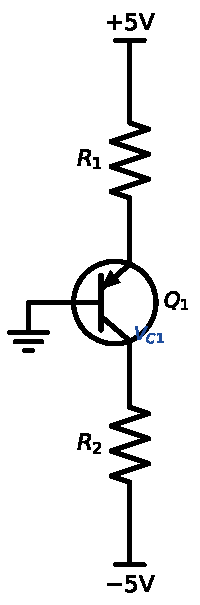
\includegraphics[width=0.9\linewidth,height=6cm,keepaspectratio]{p05_circuit}\end{center}
\solstep{1}{Rules}With $I_B\approx0$ and every transistor active ($|V_{BE}|=0.7$\,V, $I_C\approx I_E$), a resistor is known as soon as the voltages at both of its ends and the current through it are known: $R = \Delta V / I$. The specifications give the currents and some node voltages; the remaining freedom is removed with two rules:\begin{itemize}[leftmargin=*,itemsep=1pt]
\item $V_{BE}$-insensitive: the voltage across the resistor that sets an emitter current must be at least $1$\,V (then $\pm0.1$\,V of $V_{BE}$ changes $I_C$ by at most $10\,\%$);
\item $\beta$-insensitive: a divider current must be much larger ($\ge 10\times$) than the base current it feeds, and a collector current that drives a base must be much larger than that base current.
\end{itemize}
Work from the nodes that are already fixed towards the unknown ones.
\solstep{2}{Design, node by node}\begin{enumerate}[leftmargin=*,itemsep=3pt]
\item $Q_{1}$ is active: $V_{E1} = 0 + 0.7 = 0.7\,\mathrm{V}$.
\item With $I_B\approx0$ the only current through $R_{1}$ is $I_{E1}$: $I_{R1} = I_{E1} = 2\,\mathrm{m}\mathrm{A}$ ($I_C\approx I_E$).
\item $\displaystyle R_{1} = \frac{5 - V_{E1}}{I_{E1}} = \frac{5 - 0.7}{2\,\mathrm{m}\mathrm{A}} = \mathbf{2.15\,\mathrm{k}\Omega}$
\item With $I_B\approx0$ the only current through $R_{2}$ is $I_{C1}$: $I_{R2} = I_{C1} = 2\,\mathrm{m}\mathrm{A}$.
\item $\displaystyle R_{2} = \frac{V_{C1} - (-5)}{I_{C1}} = \frac{-1 - (-5)}{2\,\mathrm{m}\mathrm{A}} = \mathbf{2\,\mathrm{k}\Omega}$
\end{enumerate}

\solstep{3}{Designed circuit}\begin{center}\renewcommand{\arraystretch}{1.35}
\begin{tabular}{cc}
\toprule
resistor & value \\
\midrule
$R_{1}$ & $2.15\,\mathrm{k}\Omega$ \\
$R_{2}$ & $2\,\mathrm{k}\Omega$ \\
\bottomrule
\end{tabular}\end{center}
\begin{center}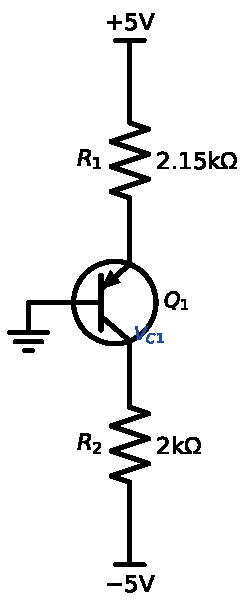
\includegraphics[width=0.85\linewidth,height=6cm,keepaspectratio]{p05_designed}\end{center}

\solstep{4}{Check the design}\begin{itemize}[leftmargin=*,itemsep=2pt]
\item $V_{EC1} = V_{E1} - V_{C1} = 0.7 - (-1) = 1.7\,\mathrm{V} \ge 0.2$\,V \checkmark
\end{itemize}
Finally the designed circuit is solved exactly ($\beta=100$, base currents included), once with $|V_{BE}|=0.7$\,V and once with each transistor's $|V_{BE}|$ changed to $0.6$ and $0.8$\,V:\begin{center}\renewcommand{\arraystretch}{1.35}
\begin{tabular}{cccccc}
\toprule
 & target $I_C$ & exact $I_C$ & $|V_{BE}|=0.6$ & $|V_{BE}|=0.8$ & max change \\
\midrule
$Q_{1}$ & $2\,\mathrm{m}\mathrm{A}$ & $1.98\,\mathrm{m}\mathrm{A}$ & $2.03\,\mathrm{m}\mathrm{A}$ & $1.93\,\mathrm{m}\mathrm{A}$ & $2.3\,\%$ \\
\bottomrule
\end{tabular}\end{center}
A $\pm0.1$\,V change of $V_{BE}$ moves no current by more than about $10\,\%$ of its design value ($V_{BE}$-insensitive), and the exact currents are close to the targets ($I_B$ negligible).
\begin{ansbox}
$R_{1} = 2.15\,\mathrm{k}\Omega$,\quad $R_{2} = 2\,\mathrm{k}\Omega$
\end{ansbox}

\newpage
\subsection*{Solution 4C.6 \hfill Easy}
\begin{center}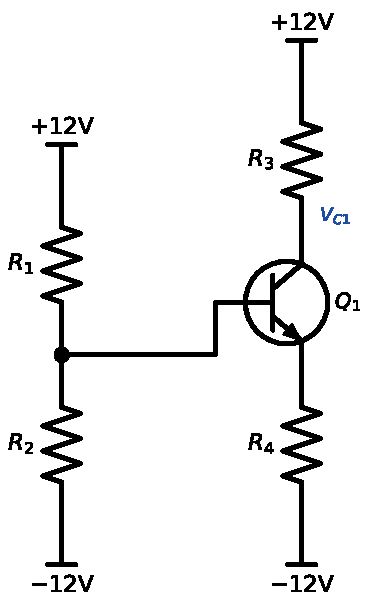
\includegraphics[width=0.9\linewidth,height=6cm,keepaspectratio]{p06_circuit}\end{center}
\solstep{1}{Rules}With $I_B\approx0$ and every transistor active ($|V_{BE}|=0.7$\,V, $I_C\approx I_E$), a resistor is known as soon as the voltages at both of its ends and the current through it are known: $R = \Delta V / I$. The specifications give the currents and some node voltages; the remaining freedom is removed with two rules:\begin{itemize}[leftmargin=*,itemsep=1pt]
\item $V_{BE}$-insensitive: the voltage across the resistor that sets an emitter current must be at least $1$\,V (then $\pm0.1$\,V of $V_{BE}$ changes $I_C$ by at most $10\,\%$);
\item $\beta$-insensitive: a divider current must be much larger ($\ge 10\times$) than the base current it feeds, and a collector current that drives a base must be much larger than that base current.
\end{itemize}
Work from the nodes that are already fixed towards the unknown ones.
\solstep{2}{Design, node by node}\begin{enumerate}[leftmargin=*,itemsep=3pt]
\item $V_{BE}$-insensitivity: a $0.1$\,V change of $V_{BE}$ changes the voltage across $R_{4}$ by $0.1$\,V, so $\frac{\Delta I_C}{I_C} = \frac{0.1}{V_{R4}} \le 10\%$ needs $V_{R4} \ge 1$\,V. Choose the smallest value, $V_{R4} = 1$\,V: $V_{E1} = (-12) + V_{R4} = -12 + 1 = -11\,\mathrm{V}$.
\item The divider current must be much larger than the base current it feeds ($I_{B1} = 20\,\mu \mathrm{A}$). Choose $I_{R2} = 1\,\mathrm{m}\mathrm{A}$ (50 times larger).
\item $Q_{1}$ is active: $V_{B1} = V_{E1} + 0.7 = -10.3\,\mathrm{V}$.
\item With $I_B\approx0$ the only current through $R_{1}$ is $I_{R2}$: $I_{R1} = I_{R2} = 1\,\mathrm{m}\mathrm{A}$.
\item $\displaystyle R_{1} = \frac{12 - V_{B1}}{I_{R2}} = \frac{12 - (-10.3)}{1\,\mathrm{m}\mathrm{A}} = \mathbf{22.3\,\mathrm{k}\Omega}$
\item $\displaystyle R_{2} = \frac{V_{B1} - (-12)}{I_{R2}} = \frac{-10.3 - (-12)}{1\,\mathrm{m}\mathrm{A}} = \mathbf{1.7\,\mathrm{k}\Omega}$
\item With $I_B\approx0$ the only current through $R_{3}$ is $I_{C1}$: $I_{R3} = I_{C1} = 2\,\mathrm{m}\mathrm{A}$.
\item $\displaystyle R_{3} = \frac{12 - V_{C1}}{I_{C1}} = \frac{12 - 4}{2\,\mathrm{m}\mathrm{A}} = \mathbf{4\,\mathrm{k}\Omega}$
\item With $I_B\approx0$ the only current through $R_{4}$ is $I_{E1}$: $I_{R4} = I_{E1} = 2\,\mathrm{m}\mathrm{A}$ ($I_C\approx I_E$).
\item $\displaystyle R_{4} = \frac{V_{E1} - (-12)}{I_{E1}} = \frac{-11 - (-12)}{2\,\mathrm{m}\mathrm{A}} = \mathbf{500\,\Omega}$
\end{enumerate}

\solstep{3}{Designed circuit}\begin{center}\renewcommand{\arraystretch}{1.35}
\begin{tabular}{cc}
\toprule
resistor & value \\
\midrule
$R_{1}$ & $22.3\,\mathrm{k}\Omega$ \\
$R_{2}$ & $1.7\,\mathrm{k}\Omega$ \\
$R_{3}$ & $4\,\mathrm{k}\Omega$ \\
$R_{4}$ & $500\,\Omega$ \\
\bottomrule
\end{tabular}\end{center}
\begin{center}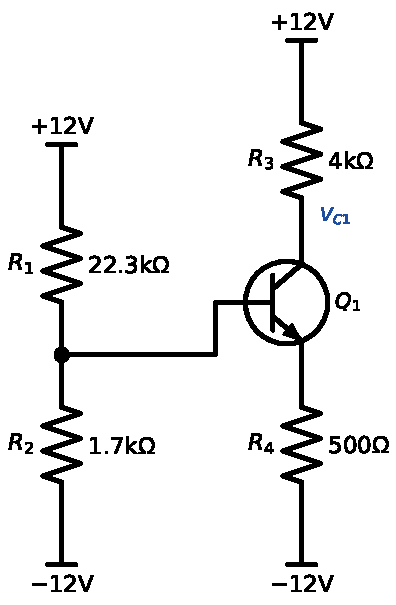
\includegraphics[width=0.85\linewidth,height=6cm,keepaspectratio]{p06_designed}\end{center}

\solstep{4}{Check the design}\begin{itemize}[leftmargin=*,itemsep=2pt]
\item $I_{B1} = \frac{I_{C1}}{\beta} = 20\,\mu \mathrm{A}$ $\ll$ the $1\,\mathrm{m}\mathrm{A}$ flowing in the base network \checkmark
\item $V_{CE1} = V_{C1} - V_{E1} = 4 - (-11) = 15\,\mathrm{V} \ge 0.2$\,V \checkmark
\end{itemize}
Finally the designed circuit is solved exactly ($\beta=100$, base currents included), once with $|V_{BE}|=0.7$\,V and once with each transistor's $|V_{BE}|$ changed to $0.6$ and $0.8$\,V:\begin{center}\renewcommand{\arraystretch}{1.35}
\begin{tabular}{cccccc}
\toprule
 & target $I_C$ & exact $I_C$ & $|V_{BE}|=0.6$ & $|V_{BE}|=0.8$ & max change \\
\midrule
$Q_{1}$ & $2\,\mathrm{m}\mathrm{A}$ & $1.92\,\mathrm{m}\mathrm{A}$ & $2.11\,\mathrm{m}\mathrm{A}$ & $1.73\,\mathrm{m}\mathrm{A}$ & $9.6\,\%$ \\
\bottomrule
\end{tabular}\end{center}
A $\pm0.1$\,V change of $V_{BE}$ moves no current by more than about $10\,\%$ of its design value ($V_{BE}$-insensitive), and the exact currents are close to the targets ($I_B$ negligible).
\begin{ansbox}
$R_{1} = 22.3\,\mathrm{k}\Omega$,\quad $R_{2} = 1.7\,\mathrm{k}\Omega$,\quad $R_{3} = 4\,\mathrm{k}\Omega$,\quad $R_{4} = 500\,\Omega$
\end{ansbox}

\newpage
\subsection*{Solution 4C.7 \hfill Medium}
\begin{center}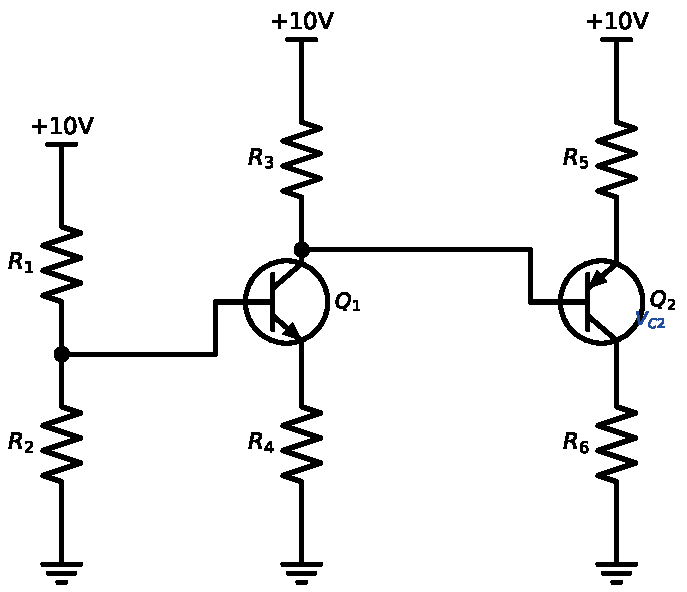
\includegraphics[width=0.9\linewidth,height=6cm,keepaspectratio]{p07_circuit}\end{center}
\solstep{1}{Rules}With $I_B\approx0$ and every transistor active ($|V_{BE}|=0.7$\,V, $I_C\approx I_E$), a resistor is known as soon as the voltages at both of its ends and the current through it are known: $R = \Delta V / I$. The specifications give the currents and some node voltages; the remaining freedom is removed with two rules:\begin{itemize}[leftmargin=*,itemsep=1pt]
\item $V_{BE}$-insensitive: the voltage across the resistor that sets an emitter current must be at least $1$\,V (then $\pm0.1$\,V of $V_{BE}$ changes $I_C$ by at most $10\,\%$);
\item $\beta$-insensitive: a divider current must be much larger ($\ge 10\times$) than the base current it feeds, and a collector current that drives a base must be much larger than that base current.
\end{itemize}
Work from the nodes that are already fixed towards the unknown ones.
\solstep{2}{Design, node by node}\begin{enumerate}[leftmargin=*,itemsep=3pt]
\item $V_{BE}$-insensitivity: a $0.1$\,V change of $V_{BE}$ changes the voltage across $R_{4}$ by $0.1$\,V, so $\frac{\Delta I_C}{I_C} = \frac{0.1}{V_{R4}} \le 10\%$ needs $V_{R4} \ge 1$\,V. Choose the smallest value, $V_{R4} = 1$\,V: $V_{E1} = 0 + V_{R4} = 0 + 1 = 1\,\mathrm{V}$.
\item $V_{BE}$-insensitivity: a $0.1$\,V change of $V_{BE}$ changes the voltage across $R_{5}$ by $0.1$\,V, so $\frac{\Delta I_C}{I_C} = \frac{0.1}{V_{R5}} \le 10\%$ needs $V_{R5} \ge 1$\,V. Choose the smallest value, $V_{R5} = 1$\,V: $V_{E2} = 10 - V_{R5} = 10 - 1 = 9\,\mathrm{V}$.
\item The divider current must be much larger than the base current it feeds ($I_{B1} = 10\,\mu \mathrm{A}$). Choose $I_{R2} = 500\,\mu \mathrm{A}$ (50 times larger).
\item $Q_{1}$ is active: $V_{B1} = V_{E1} + 0.7 = 1.7\,\mathrm{V}$.
\item $Q_{2}$ is active: $V_{C1} = V_{E2} - 0.7 = 8.3\,\mathrm{V}$.
\item With $I_B\approx0$ the only current through $R_{1}$ is $I_{R2}$: $I_{R1} = I_{R2} = 500\,\mu \mathrm{A}$.
\item $\displaystyle R_{1} = \frac{10 - V_{B1}}{I_{R2}} = \frac{10 - 1.7}{500\,\mu \mathrm{A}} = \mathbf{16.6\,\mathrm{k}\Omega}$
\item $\displaystyle R_{2} = \frac{V_{B1} - 0}{I_{R2}} = \frac{1.7 - 0}{500\,\mu \mathrm{A}} = \mathbf{3.4\,\mathrm{k}\Omega}$
\item With $I_B\approx0$ the only current through $R_{3}$ is $I_{C1}$: $I_{R3} = I_{C1} = 1\,\mathrm{m}\mathrm{A}$.
\item $\displaystyle R_{3} = \frac{10 - V_{C1}}{I_{C1}} = \frac{10 - 8.3}{1\,\mathrm{m}\mathrm{A}} = \mathbf{1.7\,\mathrm{k}\Omega}$
\item With $I_B\approx0$ the only current through $R_{4}$ is $I_{E1}$: $I_{R4} = I_{E1} = 1\,\mathrm{m}\mathrm{A}$ ($I_C\approx I_E$).
\item $\displaystyle R_{4} = \frac{V_{E1} - 0}{I_{E1}} = \frac{1 - 0}{1\,\mathrm{m}\mathrm{A}} = \mathbf{1\,\mathrm{k}\Omega}$
\item With $I_B\approx0$ the only current through $R_{5}$ is $I_{E2}$: $I_{R5} = I_{E2} = 2\,\mathrm{m}\mathrm{A}$ ($I_C\approx I_E$).
\item $\displaystyle R_{5} = \frac{10 - V_{E2}}{I_{E2}} = \frac{10 - 9}{2\,\mathrm{m}\mathrm{A}} = \mathbf{500\,\Omega}$
\item With $I_B\approx0$ the only current through $R_{6}$ is $I_{C2}$: $I_{R6} = I_{C2} = 2\,\mathrm{m}\mathrm{A}$.
\item $\displaystyle R_{6} = \frac{V_{C2} - 0}{I_{C2}} = \frac{4 - 0}{2\,\mathrm{m}\mathrm{A}} = \mathbf{2\,\mathrm{k}\Omega}$
\end{enumerate}

\solstep{3}{Designed circuit}\begin{center}\renewcommand{\arraystretch}{1.35}
\begin{tabular}{cc}
\toprule
resistor & value \\
\midrule
$R_{1}$ & $16.6\,\mathrm{k}\Omega$ \\
$R_{2}$ & $3.4\,\mathrm{k}\Omega$ \\
$R_{3}$ & $1.7\,\mathrm{k}\Omega$ \\
$R_{4}$ & $1\,\mathrm{k}\Omega$ \\
$R_{5}$ & $500\,\Omega$ \\
$R_{6}$ & $2\,\mathrm{k}\Omega$ \\
\bottomrule
\end{tabular}\end{center}
\begin{center}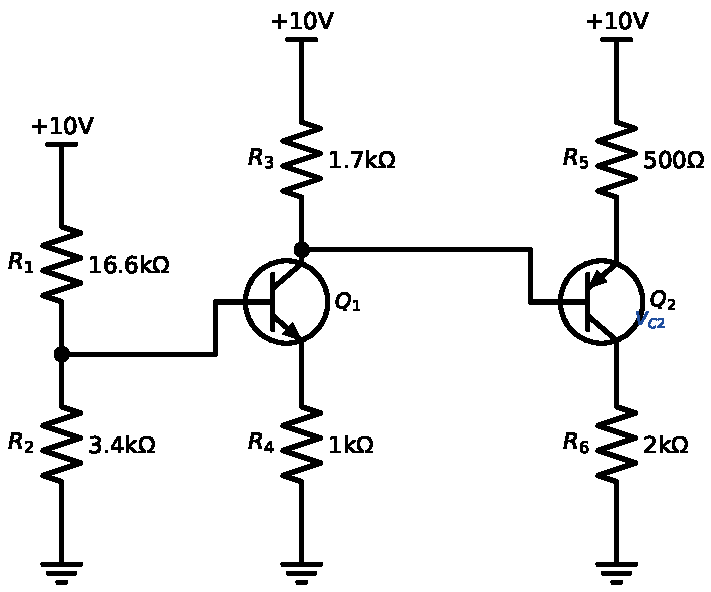
\includegraphics[width=0.85\linewidth,height=6cm,keepaspectratio]{p07_designed}\end{center}

\solstep{4}{Check the design}\begin{itemize}[leftmargin=*,itemsep=2pt]
\item $I_{B1} = \frac{I_{C1}}{\beta} = 10\,\mu \mathrm{A}$ $\ll$ the $500\,\mu \mathrm{A}$ flowing in the base network \checkmark
\item $I_{B2} = \frac{I_{C2}}{\beta} = 20\,\mu \mathrm{A}$ $\ll$ the $1\,\mathrm{m}\mathrm{A}$ flowing in the base network \checkmark
\item $V_{CE1} = V_{C1} - V_{E1} = 8.3 - 1 = 7.3\,\mathrm{V} \ge 1$\,V \checkmark
\item $V_{EC2} = V_{E2} - V_{C2} = 9 - 4 = 5\,\mathrm{V} \ge 1$\,V \checkmark
\end{itemize}
Finally the designed circuit is solved exactly ($\beta=100$, base currents included), once with $|V_{BE}|=0.7$\,V and once with each transistor's $|V_{BE}|$ changed to $0.6$ and $0.8$\,V:\begin{center}\renewcommand{\arraystretch}{1.35}
\begin{tabular}{cccccc}
\toprule
 & target $I_C$ & exact $I_C$ & $|V_{BE}|=0.6$ & $|V_{BE}|=0.8$ & max change \\
\midrule
$Q_{1}$ & $1\,\mathrm{m}\mathrm{A}$ & $963\,\mu \mathrm{A}$ & $1.06\,\mathrm{m}\mathrm{A}$ & $867\,\mu \mathrm{A}$ & $9.6\,\%$ \\
$Q_{2}$ & $2\,\mathrm{m}\mathrm{A}$ & $1.8\,\mathrm{m}\mathrm{A}$ & $1.99\,\mathrm{m}\mathrm{A}$ & $1.6\,\mathrm{m}\mathrm{A}$ & $9.6\,\%$ \\
\bottomrule
\end{tabular}\end{center}
A $\pm0.1$\,V change of $V_{BE}$ moves no current by more than about $10\,\%$ of its design value ($V_{BE}$-insensitive), and the exact currents are close to the targets ($I_B$ negligible). The exact currents drift further from the targets along a chain of direct-coupled stages: each base current and each $I_C = \alpha I_E$ slightly shifts the collector voltage that biases the next stage, and with only $\approx1$\,V across the next emitter resistor that shift is amplified. This is the normal accuracy of a hand design with $I_B\approx0$; a larger emitter-resistor voltage in the later stages reduces the drift.
\begin{ansbox}
$R_{1} = 16.6\,\mathrm{k}\Omega$,\quad $R_{2} = 3.4\,\mathrm{k}\Omega$,\quad $R_{3} = 1.7\,\mathrm{k}\Omega$,\quad $R_{4} = 1\,\mathrm{k}\Omega$,\quad $R_{5} = 500\,\Omega$,\quad $R_{6} = 2\,\mathrm{k}\Omega$
\end{ansbox}

\newpage
\subsection*{Solution 4C.8 \hfill Medium}
\begin{center}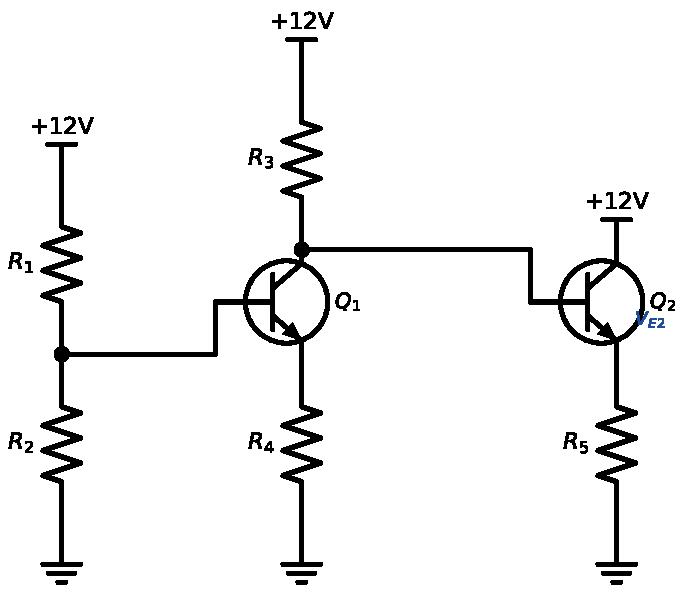
\includegraphics[width=0.9\linewidth,height=6cm,keepaspectratio]{p08_circuit}\end{center}
\solstep{1}{Rules}With $I_B\approx0$ and every transistor active ($|V_{BE}|=0.7$\,V, $I_C\approx I_E$), a resistor is known as soon as the voltages at both of its ends and the current through it are known: $R = \Delta V / I$. The specifications give the currents and some node voltages; the remaining freedom is removed with two rules:\begin{itemize}[leftmargin=*,itemsep=1pt]
\item $V_{BE}$-insensitive: the voltage across the resistor that sets an emitter current must be at least $1$\,V (then $\pm0.1$\,V of $V_{BE}$ changes $I_C$ by at most $10\,\%$);
\item $\beta$-insensitive: a divider current must be much larger ($\ge 10\times$) than the base current it feeds, and a collector current that drives a base must be much larger than that base current.
\end{itemize}
Work from the nodes that are already fixed towards the unknown ones.
\solstep{2}{Design, node by node}\begin{enumerate}[leftmargin=*,itemsep=3pt]
\item $V_{BE}$-insensitivity: a $0.1$\,V change of $V_{BE}$ changes the voltage across $R_{4}$ by $0.1$\,V, so $\frac{\Delta I_C}{I_C} = \frac{0.1}{V_{R4}} \le 10\%$ needs $V_{R4} \ge 1$\,V. Choose the smallest value, $V_{R4} = 1$\,V: $V_{E1} = 0 + V_{R4} = 0 + 1 = 1\,\mathrm{V}$.
\item The divider current must be much larger than the base current it feeds ($I_{B1} = 10\,\mu \mathrm{A}$). Choose $I_{R2} = 500\,\mu \mathrm{A}$ (50 times larger).
\item $Q_{1}$ is active: $V_{B1} = V_{E1} + 0.7 = 1.7\,\mathrm{V}$.
\item $Q_{2}$ is active: $V_{C1} = V_{E2} + 0.7 = 6.7\,\mathrm{V}$.
\item With $I_B\approx0$ the only current through $R_{1}$ is $I_{R2}$: $I_{R1} = I_{R2} = 500\,\mu \mathrm{A}$.
\item $\displaystyle R_{1} = \frac{12 - V_{B1}}{I_{R2}} = \frac{12 - 1.7}{500\,\mu \mathrm{A}} = \mathbf{20.6\,\mathrm{k}\Omega}$
\item $\displaystyle R_{2} = \frac{V_{B1} - 0}{I_{R2}} = \frac{1.7 - 0}{500\,\mu \mathrm{A}} = \mathbf{3.4\,\mathrm{k}\Omega}$
\item With $I_B\approx0$ the only current through $R_{3}$ is $I_{C1}$: $I_{R3} = I_{C1} = 1\,\mathrm{m}\mathrm{A}$.
\item $\displaystyle R_{3} = \frac{12 - V_{C1}}{I_{C1}} = \frac{12 - 6.7}{1\,\mathrm{m}\mathrm{A}} = \mathbf{5.3\,\mathrm{k}\Omega}$
\item With $I_B\approx0$ the only current through $R_{4}$ is $I_{E1}$: $I_{R4} = I_{E1} = 1\,\mathrm{m}\mathrm{A}$ ($I_C\approx I_E$).
\item $\displaystyle R_{4} = \frac{V_{E1} - 0}{I_{E1}} = \frac{1 - 0}{1\,\mathrm{m}\mathrm{A}} = \mathbf{1\,\mathrm{k}\Omega}$
\item With $I_B\approx0$ the only current through $R_{5}$ is $I_{E2}$: $I_{R5} = I_{E2} = 4\,\mathrm{m}\mathrm{A}$ ($I_C\approx I_E$).
\item $\displaystyle R_{5} = \frac{V_{E2} - 0}{I_{E2}} = \frac{6 - 0}{4\,\mathrm{m}\mathrm{A}} = \mathbf{1.5\,\mathrm{k}\Omega}$
\end{enumerate}

\solstep{3}{Designed circuit}\begin{center}\renewcommand{\arraystretch}{1.35}
\begin{tabular}{cc}
\toprule
resistor & value \\
\midrule
$R_{1}$ & $20.6\,\mathrm{k}\Omega$ \\
$R_{2}$ & $3.4\,\mathrm{k}\Omega$ \\
$R_{3}$ & $5.3\,\mathrm{k}\Omega$ \\
$R_{4}$ & $1\,\mathrm{k}\Omega$ \\
$R_{5}$ & $1.5\,\mathrm{k}\Omega$ \\
\bottomrule
\end{tabular}\end{center}
\begin{center}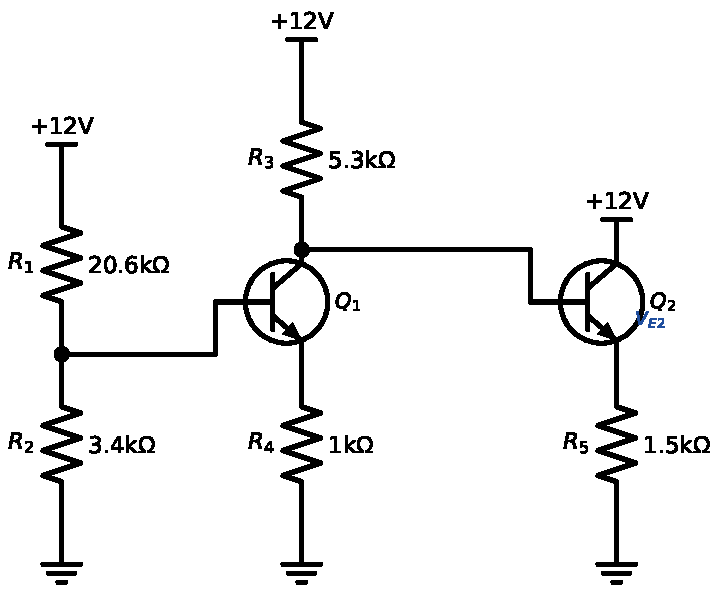
\includegraphics[width=0.85\linewidth,height=6cm,keepaspectratio]{p08_designed}\end{center}

\solstep{4}{Check the design}\begin{itemize}[leftmargin=*,itemsep=2pt]
\item $I_{B1} = \frac{I_{C1}}{\beta} = 10\,\mu \mathrm{A}$ $\ll$ the $500\,\mu \mathrm{A}$ flowing in the base network \checkmark
\item $I_{B2} = \frac{I_{C2}}{\beta} = 40\,\mu \mathrm{A}$ $\ll$ the $1\,\mathrm{m}\mathrm{A}$ flowing in the base network \checkmark
\item $V_{CE1} = V_{C1} - V_{E1} = 6.7 - 1 = 5.7\,\mathrm{V} \ge 1$\,V \checkmark
\item $V_{CE2} = 12 - V_{E2} = 12 - 6 = 6\,\mathrm{V} \ge 1$\,V \checkmark
\end{itemize}
Finally the designed circuit is solved exactly ($\beta=100$, base currents included), once with $|V_{BE}|=0.7$\,V and once with each transistor's $|V_{BE}|$ changed to $0.6$ and $0.8$\,V:\begin{center}\renewcommand{\arraystretch}{1.35}
\begin{tabular}{cccccc}
\toprule
 & target $I_C$ & exact $I_C$ & $|V_{BE}|=0.6$ & $|V_{BE}|=0.8$ & max change \\
\midrule
$Q_{1}$ & $1\,\mathrm{m}\mathrm{A}$ & $962\,\mu \mathrm{A}$ & $1.06\,\mathrm{m}\mathrm{A}$ & $866\,\mu \mathrm{A}$ & $9.6\,\%$ \\
$Q_{2}$ & $4\,\mathrm{m}\mathrm{A}$ & $3.95\,\mathrm{m}\mathrm{A}$ & $4.02\,\mathrm{m}\mathrm{A}$ & $3.89\,\mathrm{m}\mathrm{A}$ & $1.6\,\%$ \\
\bottomrule
\end{tabular}\end{center}
A $\pm0.1$\,V change of $V_{BE}$ moves no current by more than about $10\,\%$ of its design value ($V_{BE}$-insensitive), and the exact currents are close to the targets ($I_B$ negligible).
\begin{ansbox}
$R_{1} = 20.6\,\mathrm{k}\Omega$,\quad $R_{2} = 3.4\,\mathrm{k}\Omega$,\quad $R_{3} = 5.3\,\mathrm{k}\Omega$,\quad $R_{4} = 1\,\mathrm{k}\Omega$,\quad $R_{5} = 1.5\,\mathrm{k}\Omega$
\end{ansbox}

\newpage
\subsection*{Solution 4C.9 \hfill Medium}
\begin{center}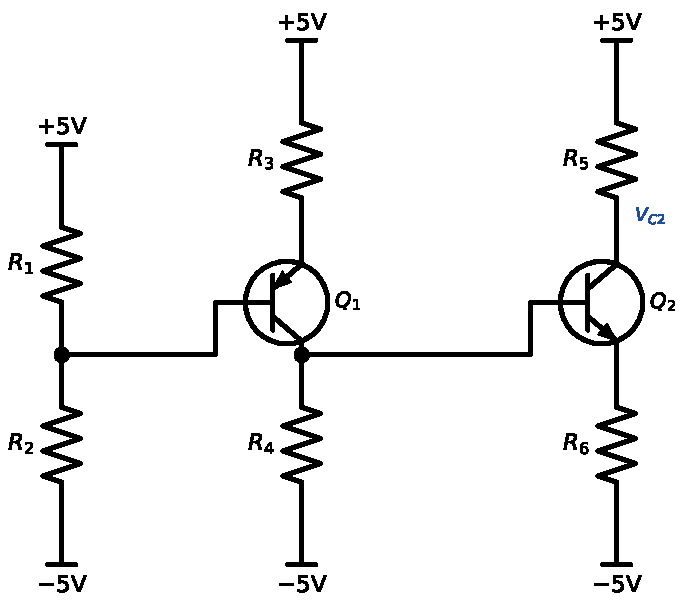
\includegraphics[width=0.9\linewidth,height=6cm,keepaspectratio]{p09_circuit}\end{center}
\solstep{1}{Rules}With $I_B\approx0$ and every transistor active ($|V_{BE}|=0.7$\,V, $I_C\approx I_E$), a resistor is known as soon as the voltages at both of its ends and the current through it are known: $R = \Delta V / I$. The specifications give the currents and some node voltages; the remaining freedom is removed with two rules:\begin{itemize}[leftmargin=*,itemsep=1pt]
\item $V_{BE}$-insensitive: the voltage across the resistor that sets an emitter current must be at least $1$\,V (then $\pm0.1$\,V of $V_{BE}$ changes $I_C$ by at most $10\,\%$);
\item $\beta$-insensitive: a divider current must be much larger ($\ge 10\times$) than the base current it feeds, and a collector current that drives a base must be much larger than that base current.
\end{itemize}
Work from the nodes that are already fixed towards the unknown ones.
\solstep{2}{Design, node by node}\begin{enumerate}[leftmargin=*,itemsep=3pt]
\item $V_{BE}$-insensitivity: a $0.1$\,V change of $V_{BE}$ changes the voltage across $R_{3}$ by $0.1$\,V, so $\frac{\Delta I_C}{I_C} = \frac{0.1}{V_{R3}} \le 10\%$ needs $V_{R3} \ge 1$\,V. Choose the smallest value, $V_{R3} = 1$\,V: $V_{E1} = 5 - V_{R3} = 5 - 1 = 4\,\mathrm{V}$.
\item $V_{BE}$-insensitivity: a $0.1$\,V change of $V_{BE}$ changes the voltage across $R_{6}$ by $0.1$\,V, so $\frac{\Delta I_C}{I_C} = \frac{0.1}{V_{R6}} \le 10\%$ needs $V_{R6} \ge 1$\,V. Choose the smallest value, $V_{R6} = 1$\,V: $V_{E2} = (-5) + V_{R6} = -5 + 1 = -4\,\mathrm{V}$.
\item The divider current must be much larger than the base current it feeds ($I_{B1} = 10\,\mu \mathrm{A}$). Choose $I_{R2} = 500\,\mu \mathrm{A}$ (50 times larger).
\item $Q_{1}$ is active: $V_{B1} = V_{E1} - 0.7 = 3.3\,\mathrm{V}$.
\item $Q_{2}$ is active: $V_{C1} = V_{E2} + 0.7 = -3.3\,\mathrm{V}$.
\item With $I_B\approx0$ the only current through $R_{1}$ is $I_{R2}$: $I_{R1} = I_{R2} = 500\,\mu \mathrm{A}$.
\item $\displaystyle R_{1} = \frac{5 - V_{B1}}{I_{R2}} = \frac{5 - 3.3}{500\,\mu \mathrm{A}} = \mathbf{3.4\,\mathrm{k}\Omega}$
\item $\displaystyle R_{2} = \frac{V_{B1} - (-5)}{I_{R2}} = \frac{3.3 - (-5)}{500\,\mu \mathrm{A}} = \mathbf{16.6\,\mathrm{k}\Omega}$
\item With $I_B\approx0$ the only current through $R_{3}$ is $I_{E1}$: $I_{R3} = I_{E1} = 1\,\mathrm{m}\mathrm{A}$ ($I_C\approx I_E$).
\item $\displaystyle R_{3} = \frac{5 - V_{E1}}{I_{E1}} = \frac{5 - 4}{1\,\mathrm{m}\mathrm{A}} = \mathbf{1\,\mathrm{k}\Omega}$
\item With $I_B\approx0$ the only current through $R_{4}$ is $I_{C1}$: $I_{R4} = I_{C1} = 1\,\mathrm{m}\mathrm{A}$.
\item $\displaystyle R_{4} = \frac{V_{C1} - (-5)}{I_{C1}} = \frac{-3.3 - (-5)}{1\,\mathrm{m}\mathrm{A}} = \mathbf{1.7\,\mathrm{k}\Omega}$
\item With $I_B\approx0$ the only current through $R_{5}$ is $I_{C2}$: $I_{R5} = I_{C2} = 2\,\mathrm{m}\mathrm{A}$.
\item $\displaystyle R_{5} = \frac{5 - V_{C2}}{I_{C2}} = \frac{5 - 1}{2\,\mathrm{m}\mathrm{A}} = \mathbf{2\,\mathrm{k}\Omega}$
\item With $I_B\approx0$ the only current through $R_{6}$ is $I_{E2}$: $I_{R6} = I_{E2} = 2\,\mathrm{m}\mathrm{A}$ ($I_C\approx I_E$).
\item $\displaystyle R_{6} = \frac{V_{E2} - (-5)}{I_{E2}} = \frac{-4 - (-5)}{2\,\mathrm{m}\mathrm{A}} = \mathbf{500\,\Omega}$
\end{enumerate}

\solstep{3}{Designed circuit}\begin{center}\renewcommand{\arraystretch}{1.35}
\begin{tabular}{cc}
\toprule
resistor & value \\
\midrule
$R_{1}$ & $3.4\,\mathrm{k}\Omega$ \\
$R_{2}$ & $16.6\,\mathrm{k}\Omega$ \\
$R_{3}$ & $1\,\mathrm{k}\Omega$ \\
$R_{4}$ & $1.7\,\mathrm{k}\Omega$ \\
$R_{5}$ & $2\,\mathrm{k}\Omega$ \\
$R_{6}$ & $500\,\Omega$ \\
\bottomrule
\end{tabular}\end{center}
\begin{center}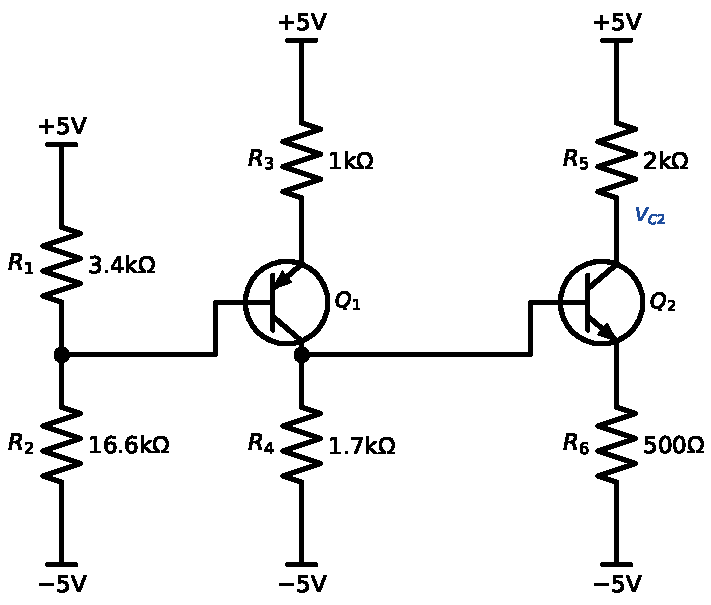
\includegraphics[width=0.85\linewidth,height=6cm,keepaspectratio]{p09_designed}\end{center}

\solstep{4}{Check the design}\begin{itemize}[leftmargin=*,itemsep=2pt]
\item $I_{B1} = \frac{I_{C1}}{\beta} = 10\,\mu \mathrm{A}$ $\ll$ the $500\,\mu \mathrm{A}$ flowing in the base network \checkmark
\item $I_{B2} = \frac{I_{C2}}{\beta} = 20\,\mu \mathrm{A}$ $\ll$ the $1\,\mathrm{m}\mathrm{A}$ flowing in the base network \checkmark
\item $V_{EC1} = V_{E1} - V_{C1} = 4 - (-3.3) = 7.3\,\mathrm{V} \ge 1$\,V \checkmark
\item $V_{CE2} = V_{C2} - V_{E2} = 1 - (-4) = 5\,\mathrm{V} \ge 1$\,V \checkmark
\end{itemize}
Finally the designed circuit is solved exactly ($\beta=100$, base currents included), once with $|V_{BE}|=0.7$\,V and once with each transistor's $|V_{BE}|$ changed to $0.6$ and $0.8$\,V:\begin{center}\renewcommand{\arraystretch}{1.35}
\begin{tabular}{cccccc}
\toprule
 & target $I_C$ & exact $I_C$ & $|V_{BE}|=0.6$ & $|V_{BE}|=0.8$ & max change \\
\midrule
$Q_{1}$ & $1\,\mathrm{m}\mathrm{A}$ & $963\,\mu \mathrm{A}$ & $1.06\,\mathrm{m}\mathrm{A}$ & $867\,\mu \mathrm{A}$ & $9.6\,\%$ \\
$Q_{2}$ & $2\,\mathrm{m}\mathrm{A}$ & $1.8\,\mathrm{m}\mathrm{A}$ & $1.99\,\mathrm{m}\mathrm{A}$ & $1.6\,\mathrm{m}\mathrm{A}$ & $9.6\,\%$ \\
\bottomrule
\end{tabular}\end{center}
A $\pm0.1$\,V change of $V_{BE}$ moves no current by more than about $10\,\%$ of its design value ($V_{BE}$-insensitive), and the exact currents are close to the targets ($I_B$ negligible). The exact currents drift further from the targets along a chain of direct-coupled stages: each base current and each $I_C = \alpha I_E$ slightly shifts the collector voltage that biases the next stage, and with only $\approx1$\,V across the next emitter resistor that shift is amplified. This is the normal accuracy of a hand design with $I_B\approx0$; a larger emitter-resistor voltage in the later stages reduces the drift.
\begin{ansbox}
$R_{1} = 3.4\,\mathrm{k}\Omega$,\quad $R_{2} = 16.6\,\mathrm{k}\Omega$,\quad $R_{3} = 1\,\mathrm{k}\Omega$,\quad $R_{4} = 1.7\,\mathrm{k}\Omega$,\quad $R_{5} = 2\,\mathrm{k}\Omega$,\quad $R_{6} = 500\,\Omega$
\end{ansbox}

\newpage
\subsection*{Solution 4C.10 \hfill Medium}
\begin{center}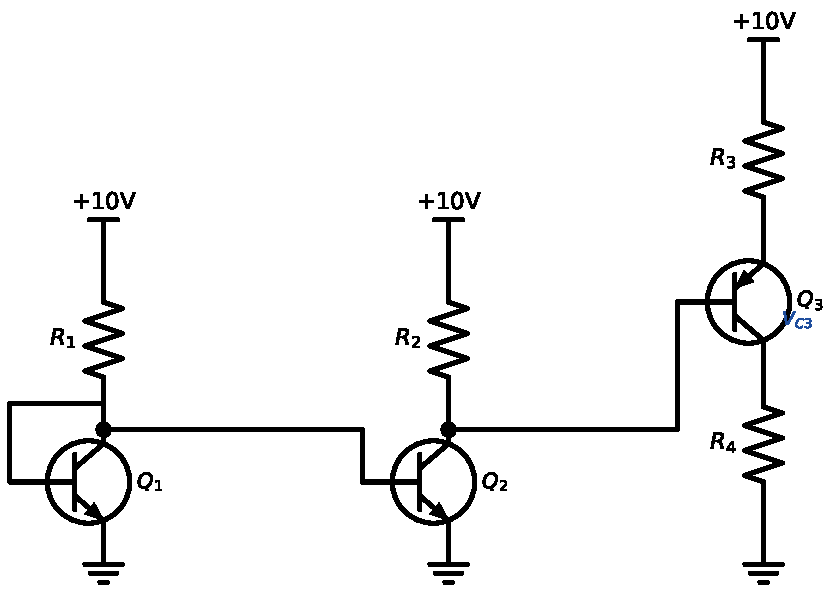
\includegraphics[width=0.9\linewidth,height=6cm,keepaspectratio]{p10_circuit}\end{center}
\solstep{1}{Rules}With $I_B\approx0$ and every transistor active ($|V_{BE}|=0.7$\,V, $I_C\approx I_E$), a resistor is known as soon as the voltages at both of its ends and the current through it are known: $R = \Delta V / I$. The specifications give the currents and some node voltages; the remaining freedom is removed with two rules:\begin{itemize}[leftmargin=*,itemsep=1pt]
\item $V_{BE}$-insensitive: the voltage across the resistor that sets an emitter current must be at least $1$\,V (then $\pm0.1$\,V of $V_{BE}$ changes $I_C$ by at most $10\,\%$);
\item $\beta$-insensitive: a divider current must be much larger ($\ge 10\times$) than the base current it feeds, and a collector current that drives a base must be much larger than that base current.
\end{itemize}
Work from the nodes that are already fixed towards the unknown ones.
\solstep{2}{Design, node by node}\begin{enumerate}[leftmargin=*,itemsep=3pt]
\item $V_{BE}$-insensitivity: a $0.1$\,V change of $V_{BE}$ changes the voltage across $R_{3}$ by $0.1$\,V, so $\frac{\Delta I_C}{I_C} = \frac{0.1}{V_{R3}} \le 10\%$ needs $V_{R3} \ge 1$\,V. Choose the smallest value, $V_{R3} = 1$\,V: $V_{E3} = 10 - V_{R3} = 10 - 1 = 9\,\mathrm{V}$.
\item $Q_{1}$ (diode-connected) is active: $V_{B1} = 0 + 0.7 = 0.7\,\mathrm{V}$.
\item $Q_{3}$ is active: $V_{C2} = V_{E3} - 0.7 = 8.3\,\mathrm{V}$.
\item $Q_{2}$ mirrors $Q_{1}$ (same base and emitter nodes): $I_{C2} = I_{C1} = 1\,\mathrm{m}\mathrm{A}$.
\item With $I_B\approx0$ the only current through $R_{1}$ is $I_{C1}$: $I_{R1} = I_{C1} = 1\,\mathrm{m}\mathrm{A}$.
\item $\displaystyle R_{1} = \frac{10 - V_{B1}}{I_{C1}} = \frac{10 - 0.7}{1\,\mathrm{m}\mathrm{A}} = \mathbf{9.3\,\mathrm{k}\Omega}$
\item With $I_B\approx0$ the only current through $R_{2}$ is $I_{C2}$: $I_{R2} = I_{C2} = 1\,\mathrm{m}\mathrm{A}$.
\item $\displaystyle R_{2} = \frac{10 - V_{C2}}{I_{C2}} = \frac{10 - 8.3}{1\,\mathrm{m}\mathrm{A}} = \mathbf{1.7\,\mathrm{k}\Omega}$
\item With $I_B\approx0$ the only current through $R_{3}$ is $I_{E3}$: $I_{R3} = I_{E3} = 2\,\mathrm{m}\mathrm{A}$ ($I_C\approx I_E$).
\item $\displaystyle R_{3} = \frac{10 - V_{E3}}{I_{E3}} = \frac{10 - 9}{2\,\mathrm{m}\mathrm{A}} = \mathbf{500\,\Omega}$
\item With $I_B\approx0$ the only current through $R_{4}$ is $I_{C3}$: $I_{R4} = I_{C3} = 2\,\mathrm{m}\mathrm{A}$.
\item $\displaystyle R_{4} = \frac{V_{C3} - 0}{I_{C3}} = \frac{3 - 0}{2\,\mathrm{m}\mathrm{A}} = \mathbf{1.5\,\mathrm{k}\Omega}$
\end{enumerate}

\solstep{3}{Designed circuit}\begin{center}\renewcommand{\arraystretch}{1.35}
\begin{tabular}{cc}
\toprule
resistor & value \\
\midrule
$R_{1}$ & $9.3\,\mathrm{k}\Omega$ \\
$R_{2}$ & $1.7\,\mathrm{k}\Omega$ \\
$R_{3}$ & $500\,\Omega$ \\
$R_{4}$ & $1.5\,\mathrm{k}\Omega$ \\
\bottomrule
\end{tabular}\end{center}
\begin{center}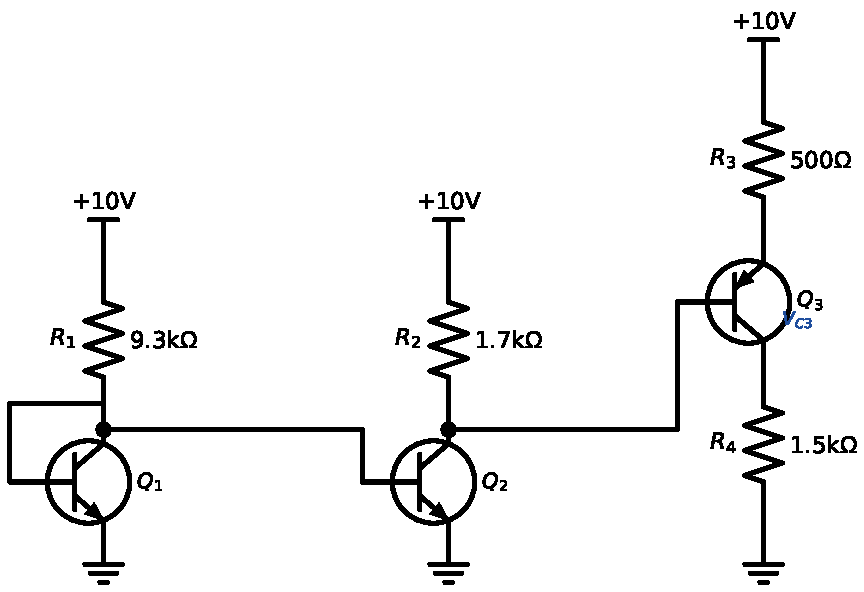
\includegraphics[width=0.85\linewidth,height=6cm,keepaspectratio]{p10_designed}\end{center}

\solstep{4}{Check the design}\begin{itemize}[leftmargin=*,itemsep=2pt]
\item $I_{B1} = \frac{I_{C1}}{\beta} = 10\,\mu \mathrm{A}$ (all bases on this node: $20\,\mu \mathrm{A}$) $\ll$ the $1\,\mathrm{m}\mathrm{A}$ flowing in the base network \checkmark
\item $I_{B2} = \frac{I_{C2}}{\beta} = 10\,\mu \mathrm{A}$ (all bases on this node: $20\,\mu \mathrm{A}$) $\ll$ the $1\,\mathrm{m}\mathrm{A}$ flowing in the base network \checkmark
\item $I_{B3} = \frac{I_{C3}}{\beta} = 20\,\mu \mathrm{A}$ $\ll$ the $1\,\mathrm{m}\mathrm{A}$ flowing in the base network \checkmark
\item $Q_{1}$ is diode-connected: $V_{CE1} = |V_{BE}| = 0.7$\,V, always active (the $|V_{CE}|$ specification is meant for the other transistors) \checkmark
\item $V_{CE2} = V_{C2} - 0 = 8.3 - 0 = 8.3\,\mathrm{V} \ge 1$\,V \checkmark
\item $V_{EC3} = V_{E3} - V_{C3} = 9 - 3 = 6\,\mathrm{V} \ge 1$\,V \checkmark
\end{itemize}
Finally the designed circuit is solved exactly ($\beta=100$, base currents included), once with $|V_{BE}|=0.7$\,V and once with each transistor's $|V_{BE}|$ changed to $0.6$ and $0.8$\,V:\begin{center}\renewcommand{\arraystretch}{1.35}
\begin{tabular}{cccccc}
\toprule
 & target $I_C$ & exact $I_C$ & $|V_{BE}|=0.6$ & $|V_{BE}|=0.8$ & max change \\
\midrule
$Q_{1}$ & $1\,\mathrm{m}\mathrm{A}$ & $980\,\mu \mathrm{A}$ & $991\,\mu \mathrm{A}$ & $970\,\mu \mathrm{A}$ & $1.1\,\%$ \\
$Q_{2}$ & $1\,\mathrm{m}\mathrm{A}$ & $980\,\mu \mathrm{A}$ & $991\,\mu \mathrm{A}$ & $970\,\mu \mathrm{A}$ & $1.1\,\%$ \\
$Q_{3}$ & $2\,\mathrm{m}\mathrm{A}$ & $1.85\,\mathrm{m}\mathrm{A}$ & $2.04\,\mathrm{m}\mathrm{A}$ & $1.66\,\mathrm{m}\mathrm{A}$ & $9.6\,\%$ \\
\bottomrule
\end{tabular}\end{center}
A $\pm0.1$\,V change of $V_{BE}$ moves no current by more than about $10\,\%$ of its design value ($V_{BE}$-insensitive), and the exact currents are close to the targets ($I_B$ negligible). The exact currents drift further from the targets along a chain of direct-coupled stages: each base current and each $I_C = \alpha I_E$ slightly shifts the collector voltage that biases the next stage, and with only $\approx1$\,V across the next emitter resistor that shift is amplified. This is the normal accuracy of a hand design with $I_B\approx0$; a larger emitter-resistor voltage in the later stages reduces the drift.
\begin{ansbox}
$R_{1} = 9.3\,\mathrm{k}\Omega$,\quad $R_{2} = 1.7\,\mathrm{k}\Omega$,\quad $R_{3} = 500\,\Omega$,\quad $R_{4} = 1.5\,\mathrm{k}\Omega$
\end{ansbox}

\newpage
\subsection*{Solution 4C.11 \hfill Medium}
\begin{center}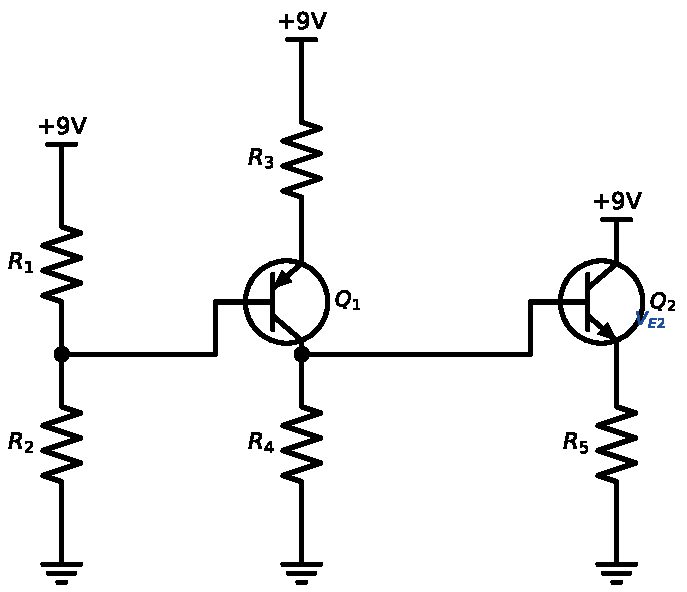
\includegraphics[width=0.9\linewidth,height=6cm,keepaspectratio]{p11_circuit}\end{center}
\solstep{1}{Rules}With $I_B\approx0$ and every transistor active ($|V_{BE}|=0.7$\,V, $I_C\approx I_E$), a resistor is known as soon as the voltages at both of its ends and the current through it are known: $R = \Delta V / I$. The specifications give the currents and some node voltages; the remaining freedom is removed with two rules:\begin{itemize}[leftmargin=*,itemsep=1pt]
\item $V_{BE}$-insensitive: the voltage across the resistor that sets an emitter current must be at least $1$\,V (then $\pm0.1$\,V of $V_{BE}$ changes $I_C$ by at most $10\,\%$);
\item $\beta$-insensitive: a divider current must be much larger ($\ge 10\times$) than the base current it feeds, and a collector current that drives a base must be much larger than that base current.
\end{itemize}
Work from the nodes that are already fixed towards the unknown ones.
\solstep{2}{Design, node by node}\begin{enumerate}[leftmargin=*,itemsep=3pt]
\item $V_{BE}$-insensitivity: a $0.1$\,V change of $V_{BE}$ changes the voltage across $R_{3}$ by $0.1$\,V, so $\frac{\Delta I_C}{I_C} = \frac{0.1}{V_{R3}} \le 10\%$ needs $V_{R3} \ge 1$\,V. Choose the smallest value, $V_{R3} = 1$\,V: $V_{E1} = 9 - V_{R3} = 9 - 1 = 8\,\mathrm{V}$.
\item The divider current must be much larger than the base current it feeds ($I_{B1} = 10\,\mu \mathrm{A}$). Choose $I_{R2} = 500\,\mu \mathrm{A}$ (50 times larger).
\item $Q_{1}$ is active: $V_{B1} = V_{E1} - 0.7 = 7.3\,\mathrm{V}$.
\item $Q_{2}$ is active: $V_{C1} = V_{E2} + 0.7 = 3.7\,\mathrm{V}$.
\item With $I_B\approx0$ the only current through $R_{1}$ is $I_{R2}$: $I_{R1} = I_{R2} = 500\,\mu \mathrm{A}$.
\item $\displaystyle R_{1} = \frac{9 - V_{B1}}{I_{R2}} = \frac{9 - 7.3}{500\,\mu \mathrm{A}} = \mathbf{3.4\,\mathrm{k}\Omega}$
\item $\displaystyle R_{2} = \frac{V_{B1} - 0}{I_{R2}} = \frac{7.3 - 0}{500\,\mu \mathrm{A}} = \mathbf{14.6\,\mathrm{k}\Omega}$
\item With $I_B\approx0$ the only current through $R_{3}$ is $I_{E1}$: $I_{R3} = I_{E1} = 1\,\mathrm{m}\mathrm{A}$ ($I_C\approx I_E$).
\item $\displaystyle R_{3} = \frac{9 - V_{E1}}{I_{E1}} = \frac{9 - 8}{1\,\mathrm{m}\mathrm{A}} = \mathbf{1\,\mathrm{k}\Omega}$
\item With $I_B\approx0$ the only current through $R_{4}$ is $I_{C1}$: $I_{R4} = I_{C1} = 1\,\mathrm{m}\mathrm{A}$.
\item $\displaystyle R_{4} = \frac{V_{C1} - 0}{I_{C1}} = \frac{3.7 - 0}{1\,\mathrm{m}\mathrm{A}} = \mathbf{3.7\,\mathrm{k}\Omega}$
\item With $I_B\approx0$ the only current through $R_{5}$ is $I_{E2}$: $I_{R5} = I_{E2} = 3\,\mathrm{m}\mathrm{A}$ ($I_C\approx I_E$).
\item $\displaystyle R_{5} = \frac{V_{E2} - 0}{I_{E2}} = \frac{3 - 0}{3\,\mathrm{m}\mathrm{A}} = \mathbf{1\,\mathrm{k}\Omega}$
\end{enumerate}

\solstep{3}{Designed circuit}\begin{center}\renewcommand{\arraystretch}{1.35}
\begin{tabular}{cc}
\toprule
resistor & value \\
\midrule
$R_{1}$ & $3.4\,\mathrm{k}\Omega$ \\
$R_{2}$ & $14.6\,\mathrm{k}\Omega$ \\
$R_{3}$ & $1\,\mathrm{k}\Omega$ \\
$R_{4}$ & $3.7\,\mathrm{k}\Omega$ \\
$R_{5}$ & $1\,\mathrm{k}\Omega$ \\
\bottomrule
\end{tabular}\end{center}
\begin{center}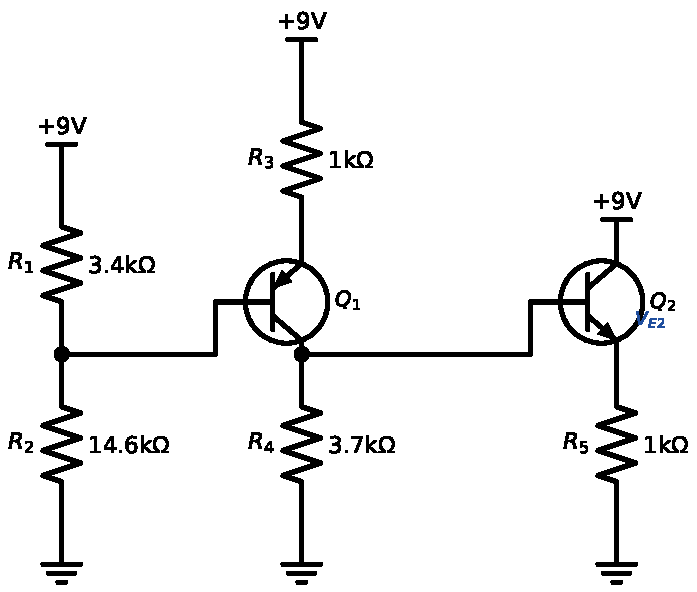
\includegraphics[width=0.85\linewidth,height=6cm,keepaspectratio]{p11_designed}\end{center}

\solstep{4}{Check the design}\begin{itemize}[leftmargin=*,itemsep=2pt]
\item $I_{B1} = \frac{I_{C1}}{\beta} = 10\,\mu \mathrm{A}$ $\ll$ the $500\,\mu \mathrm{A}$ flowing in the base network \checkmark
\item $I_{B2} = \frac{I_{C2}}{\beta} = 30\,\mu \mathrm{A}$ $\ll$ the $1\,\mathrm{m}\mathrm{A}$ flowing in the base network \checkmark
\item $V_{EC1} = V_{E1} - V_{C1} = 8 - 3.7 = 4.3\,\mathrm{V} \ge 1$\,V \checkmark
\item $V_{CE2} = 9 - V_{E2} = 9 - 3 = 6\,\mathrm{V} \ge 1$\,V \checkmark
\end{itemize}
Finally the designed circuit is solved exactly ($\beta=100$, base currents included), once with $|V_{BE}|=0.7$\,V and once with each transistor's $|V_{BE}|$ changed to $0.6$ and $0.8$\,V:\begin{center}\renewcommand{\arraystretch}{1.35}
\begin{tabular}{cccccc}
\toprule
 & target $I_C$ & exact $I_C$ & $|V_{BE}|=0.6$ & $|V_{BE}|=0.8$ & max change \\
\midrule
$Q_{1}$ & $1\,\mathrm{m}\mathrm{A}$ & $964\,\mu \mathrm{A}$ & $1.06\,\mathrm{m}\mathrm{A}$ & $867\,\mu \mathrm{A}$ & $9.6\,\%$ \\
$Q_{2}$ & $3\,\mathrm{m}\mathrm{A}$ & $2.74\,\mathrm{m}\mathrm{A}$ & $2.83\,\mathrm{m}\mathrm{A}$ & $2.64\,\mathrm{m}\mathrm{A}$ & $3.2\,\%$ \\
\bottomrule
\end{tabular}\end{center}
A $\pm0.1$\,V change of $V_{BE}$ moves no current by more than about $10\,\%$ of its design value ($V_{BE}$-insensitive), and the exact currents are close to the targets ($I_B$ negligible). The exact currents drift further from the targets along a chain of direct-coupled stages: each base current and each $I_C = \alpha I_E$ slightly shifts the collector voltage that biases the next stage, and with only $\approx1$\,V across the next emitter resistor that shift is amplified. This is the normal accuracy of a hand design with $I_B\approx0$; a larger emitter-resistor voltage in the later stages reduces the drift.
\begin{ansbox}
$R_{1} = 3.4\,\mathrm{k}\Omega$,\quad $R_{2} = 14.6\,\mathrm{k}\Omega$,\quad $R_{3} = 1\,\mathrm{k}\Omega$,\quad $R_{4} = 3.7\,\mathrm{k}\Omega$,\quad $R_{5} = 1\,\mathrm{k}\Omega$
\end{ansbox}

\newpage
\subsection*{Solution 4C.12 \hfill Medium}
\begin{center}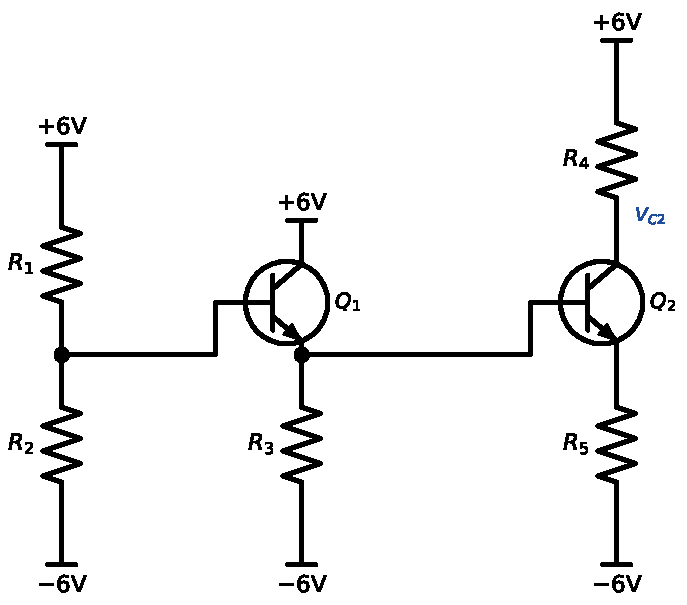
\includegraphics[width=0.9\linewidth,height=6cm,keepaspectratio]{p12_circuit}\end{center}
\solstep{1}{Rules}With $I_B\approx0$ and every transistor active ($|V_{BE}|=0.7$\,V, $I_C\approx I_E$), a resistor is known as soon as the voltages at both of its ends and the current through it are known: $R = \Delta V / I$. The specifications give the currents and some node voltages; the remaining freedom is removed with two rules:\begin{itemize}[leftmargin=*,itemsep=1pt]
\item $V_{BE}$-insensitive: the voltage across the resistor that sets an emitter current must be at least $1$\,V (then $\pm0.1$\,V of $V_{BE}$ changes $I_C$ by at most $10\,\%$);
\item $\beta$-insensitive: a divider current must be much larger ($\ge 10\times$) than the base current it feeds, and a collector current that drives a base must be much larger than that base current.
\end{itemize}
Work from the nodes that are already fixed towards the unknown ones.
\solstep{2}{Design, node by node}\begin{enumerate}[leftmargin=*,itemsep=3pt]
\item $V_{BE}$-insensitivity: a $0.1$\,V change of $V_{BE}$ changes the voltage across $R_{5}$ by $0.1$\,V, so $\frac{\Delta I_C}{I_C} = \frac{0.1}{V_{R5}} \le 10\%$ needs $V_{R5} \ge 1$\,V. Choose the smallest value, $V_{R5} = 1$\,V: $V_{E2} = (-6) + V_{R5} = -6 + 1 = -5\,\mathrm{V}$.
\item The divider current must be much larger than the base current it feeds ($I_{B1} = 10\,\mu \mathrm{A}$). Choose $I_{R2} = 500\,\mu \mathrm{A}$ (50 times larger).
\item $Q_{2}$ is active: $V_{E1} = V_{E2} + 0.7 = -4.3\,\mathrm{V}$.
\item With $I_B\approx0$ the only current through $R_{1}$ is $I_{R2}$: $I_{R1} = I_{R2} = 500\,\mu \mathrm{A}$.
\item $Q_{1}$ is active: $V_{B1} = V_{E1} + 0.7 = -3.6\,\mathrm{V}$.
\item With $I_B\approx0$ the only current through $R_{3}$ is $I_{E1}$: $I_{R3} = I_{E1} = 1\,\mathrm{m}\mathrm{A}$ ($I_C\approx I_E$).
\item $\displaystyle R_{1} = \frac{6 - V_{B1}}{I_{R2}} = \frac{6 - (-3.6)}{500\,\mu \mathrm{A}} = \mathbf{19.2\,\mathrm{k}\Omega}$
\item $\displaystyle R_{2} = \frac{V_{B1} - (-6)}{I_{R2}} = \frac{-3.6 - (-6)}{500\,\mu \mathrm{A}} = \mathbf{4.8\,\mathrm{k}\Omega}$
\item $\displaystyle R_{3} = \frac{V_{E1} - (-6)}{I_{E1}} = \frac{-4.3 - (-6)}{1\,\mathrm{m}\mathrm{A}} = \mathbf{1.7\,\mathrm{k}\Omega}$
\item With $I_B\approx0$ the only current through $R_{4}$ is $I_{C2}$: $I_{R4} = I_{C2} = 2\,\mathrm{m}\mathrm{A}$.
\item $\displaystyle R_{4} = \frac{6 - V_{C2}}{I_{C2}} = \frac{6 - 2}{2\,\mathrm{m}\mathrm{A}} = \mathbf{2\,\mathrm{k}\Omega}$
\item With $I_B\approx0$ the only current through $R_{5}$ is $I_{E2}$: $I_{R5} = I_{E2} = 2\,\mathrm{m}\mathrm{A}$ ($I_C\approx I_E$).
\item $\displaystyle R_{5} = \frac{V_{E2} - (-6)}{I_{E2}} = \frac{-5 - (-6)}{2\,\mathrm{m}\mathrm{A}} = \mathbf{500\,\Omega}$
\end{enumerate}

\solstep{3}{Designed circuit}\begin{center}\renewcommand{\arraystretch}{1.35}
\begin{tabular}{cc}
\toprule
resistor & value \\
\midrule
$R_{1}$ & $19.2\,\mathrm{k}\Omega$ \\
$R_{2}$ & $4.8\,\mathrm{k}\Omega$ \\
$R_{3}$ & $1.7\,\mathrm{k}\Omega$ \\
$R_{4}$ & $2\,\mathrm{k}\Omega$ \\
$R_{5}$ & $500\,\Omega$ \\
\bottomrule
\end{tabular}\end{center}
\begin{center}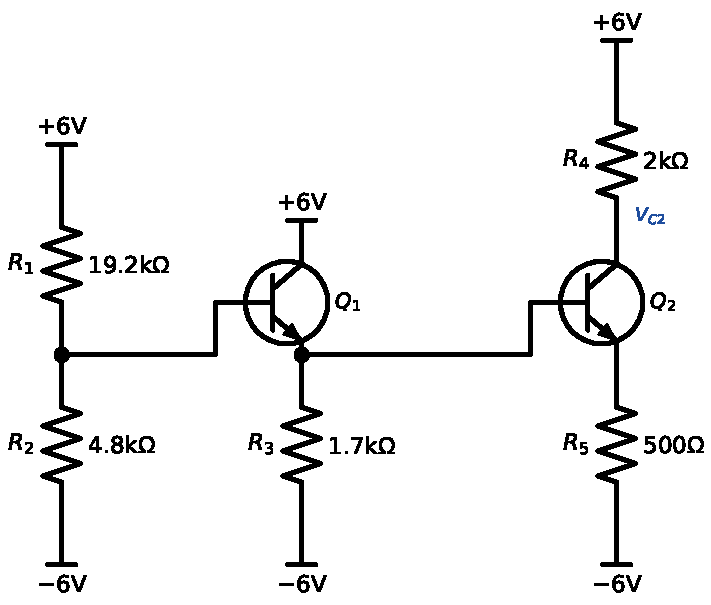
\includegraphics[width=0.85\linewidth,height=6cm,keepaspectratio]{p12_designed}\end{center}

\solstep{4}{Check the design}\begin{itemize}[leftmargin=*,itemsep=2pt]
\item $I_{B1} = \frac{I_{C1}}{\beta} = 10\,\mu \mathrm{A}$ $\ll$ the $500\,\mu \mathrm{A}$ flowing in the base network \checkmark
\item $I_{B2} = \frac{I_{C2}}{\beta} = 20\,\mu \mathrm{A}$ $\ll$ the $1\,\mathrm{m}\mathrm{A}$ flowing in the base network \checkmark
\item $V_{CE1} = 6 - V_{E1} = 6 - (-4.3) = 10.3\,\mathrm{V} \ge 1$\,V \checkmark
\item $V_{CE2} = V_{C2} - V_{E2} = 2 - (-5) = 7\,\mathrm{V} \ge 1$\,V \checkmark
\end{itemize}
Finally the designed circuit is solved exactly ($\beta=100$, base currents included), once with $|V_{BE}|=0.7$\,V and once with each transistor's $|V_{BE}|$ changed to $0.6$ and $0.8$\,V:\begin{center}\renewcommand{\arraystretch}{1.35}
\begin{tabular}{cccccc}
\toprule
 & target $I_C$ & exact $I_C$ & $|V_{BE}|=0.6$ & $|V_{BE}|=0.8$ & max change \\
\midrule
$Q_{1}$ & $1\,\mathrm{m}\mathrm{A}$ & $987\,\mu \mathrm{A}$ & $1.05\,\mathrm{m}\mathrm{A}$ & $928\,\mu \mathrm{A}$ & $5.9\,\%$ \\
$Q_{2}$ & $2\,\mathrm{m}\mathrm{A}$ & $1.91\,\mathrm{m}\mathrm{A}$ & $2.1\,\mathrm{m}\mathrm{A}$ & $1.71\,\mathrm{m}\mathrm{A}$ & $9.9\,\%$ \\
\bottomrule
\end{tabular}\end{center}
A $\pm0.1$\,V change of $V_{BE}$ moves no current by more than about $10\,\%$ of its design value ($V_{BE}$-insensitive), and the exact currents are close to the targets ($I_B$ negligible).
\begin{ansbox}
$R_{1} = 19.2\,\mathrm{k}\Omega$,\quad $R_{2} = 4.8\,\mathrm{k}\Omega$,\quad $R_{3} = 1.7\,\mathrm{k}\Omega$,\quad $R_{4} = 2\,\mathrm{k}\Omega$,\quad $R_{5} = 500\,\Omega$
\end{ansbox}

\newpage
\subsection*{Solution 4C.13 \hfill Hard}
\begin{center}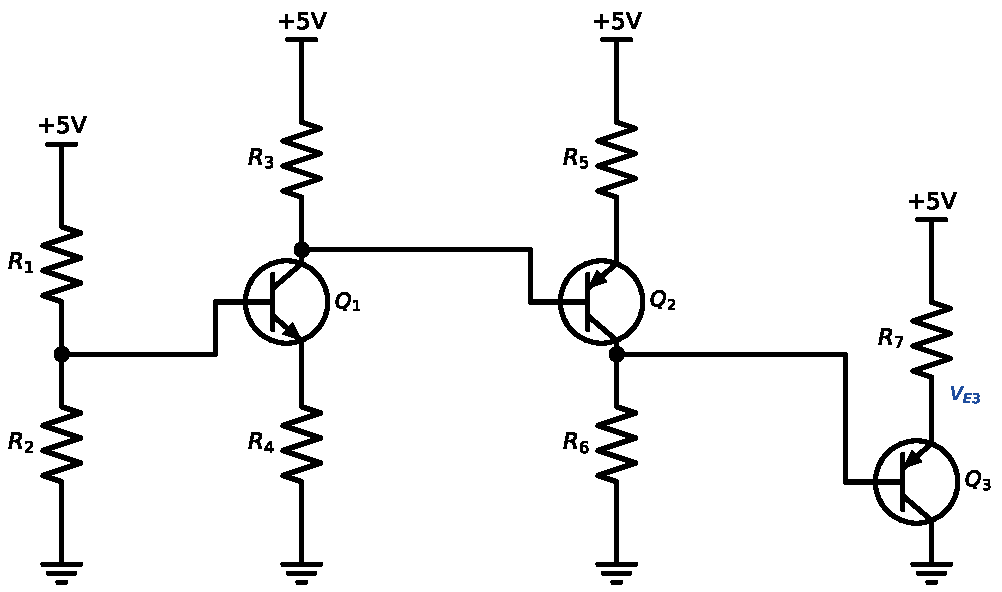
\includegraphics[width=0.9\linewidth,height=6cm,keepaspectratio]{p13_circuit}\end{center}
\solstep{1}{Rules}With $I_B\approx0$ and every transistor active ($|V_{BE}|=0.7$\,V, $I_C\approx I_E$), a resistor is known as soon as the voltages at both of its ends and the current through it are known: $R = \Delta V / I$. The specifications give the currents and some node voltages; the remaining freedom is removed with two rules:\begin{itemize}[leftmargin=*,itemsep=1pt]
\item $V_{BE}$-insensitive: the voltage across the resistor that sets an emitter current must be at least $1$\,V (then $\pm0.1$\,V of $V_{BE}$ changes $I_C$ by at most $10\,\%$);
\item $\beta$-insensitive: a divider current must be much larger ($\ge 10\times$) than the base current it feeds, and a collector current that drives a base must be much larger than that base current.
\end{itemize}
Work from the nodes that are already fixed towards the unknown ones.
\solstep{2}{Design, node by node}\begin{enumerate}[leftmargin=*,itemsep=3pt]
\item $V_{BE}$-insensitivity: a $0.1$\,V change of $V_{BE}$ changes the voltage across $R_{5}$ by $0.1$\,V, so $\frac{\Delta I_C}{I_C} = \frac{0.1}{V_{R5}} \le 10\%$ needs $V_{R5} \ge 1$\,V. Choose the smallest value, $V_{R5} = 1$\,V: $V_{E2} = 5 - V_{R5} = 5 - 1 = 4\,\mathrm{V}$.
\item $V_{BE}$-insensitivity: a $0.1$\,V change of $V_{BE}$ changes the voltage across $R_{4}$ by $0.1$\,V, so $\frac{\Delta I_C}{I_C} = \frac{0.1}{V_{R4}} \le 10\%$ needs $V_{R4} \ge 1$\,V. Choose the smallest value, $V_{R4} = 1$\,V: $V_{E1} = 0 + V_{R4} = 0 + 1 = 1\,\mathrm{V}$.
\item $I_{dc} = I_{R1} + I_{C1} + I_{C2} + I_{C3} \le 14\,\mathrm{mA}$ leaves at most $14 - 2 - 4 - 6 = 2\,\mathrm{mA}$ for the divider, and $I_{R2}$ must be $\gg I_{B1} = 20\,\mu\mathrm{A}$. Choose $I_{R2} = 1\,\mathrm{mA}$.
\item $Q_{1}$ is active: $V_{B1} = V_{E1} + 0.7 = 1.7\,\mathrm{V}$.
\item $Q_{2}$ is active: $V_{C1} = V_{E2} - 0.7 = 3.3\,\mathrm{V}$.
\item $Q_{3}$ is active: $V_{C2} = V_{E3} - 0.7 = 1.8\,\mathrm{V}$.
\item With $I_B\approx0$ the only current through $R_{1}$ is $I_{R2}$: $I_{R1} = I_{R2} = 1\,\mathrm{m}\mathrm{A}$.
\item $\displaystyle R_{1} = \frac{5 - V_{B1}}{I_{R2}} = \frac{5 - 1.7}{1\,\mathrm{m}\mathrm{A}} = \mathbf{3.3\,\mathrm{k}\Omega}$
\item $\displaystyle R_{2} = \frac{V_{B1} - 0}{I_{R2}} = \frac{1.7 - 0}{1\,\mathrm{m}\mathrm{A}} = \mathbf{1.7\,\mathrm{k}\Omega}$
\item With $I_B\approx0$ the only current through $R_{3}$ is $I_{C1}$: $I_{R3} = I_{C1} = 2\,\mathrm{m}\mathrm{A}$.
\item $\displaystyle R_{3} = \frac{5 - V_{C1}}{I_{C1}} = \frac{5 - 3.3}{2\,\mathrm{m}\mathrm{A}} = \mathbf{850\,\Omega}$
\item With $I_B\approx0$ the only current through $R_{4}$ is $I_{E1}$: $I_{R4} = I_{E1} = 2\,\mathrm{m}\mathrm{A}$ ($I_C\approx I_E$).
\item $\displaystyle R_{4} = \frac{V_{E1} - 0}{I_{E1}} = \frac{1 - 0}{2\,\mathrm{m}\mathrm{A}} = \mathbf{500\,\Omega}$
\item With $I_B\approx0$ the only current through $R_{5}$ is $I_{E2}$: $I_{R5} = I_{E2} = 4\,\mathrm{m}\mathrm{A}$ ($I_C\approx I_E$).
\item $\displaystyle R_{5} = \frac{5 - V_{E2}}{I_{E2}} = \frac{5 - 4}{4\,\mathrm{m}\mathrm{A}} = \mathbf{250\,\Omega}$
\item With $I_B\approx0$ the only current through $R_{6}$ is $I_{C2}$: $I_{R6} = I_{C2} = 4\,\mathrm{m}\mathrm{A}$.
\item $\displaystyle R_{6} = \frac{V_{C2} - 0}{I_{C2}} = \frac{1.8 - 0}{4\,\mathrm{m}\mathrm{A}} = \mathbf{450\,\Omega}$
\item With $I_B\approx0$ the only current through $R_{7}$ is $I_{E3}$: $I_{R7} = I_{E3} = 6\,\mathrm{m}\mathrm{A}$ ($I_C\approx I_E$).
\item $\displaystyle R_{7} = \frac{5 - V_{E3}}{I_{E3}} = \frac{5 - 2.5}{6\,\mathrm{m}\mathrm{A}} = \mathbf{417\,\Omega}$
\end{enumerate}

\solstep{3}{Designed circuit}\begin{center}\renewcommand{\arraystretch}{1.35}
\begin{tabular}{cc}
\toprule
resistor & value \\
\midrule
$R_{1}$ & $3.3\,\mathrm{k}\Omega$ \\
$R_{2}$ & $1.7\,\mathrm{k}\Omega$ \\
$R_{3}$ & $850\,\Omega$ \\
$R_{4}$ & $500\,\Omega$ \\
$R_{5}$ & $250\,\Omega$ \\
$R_{6}$ & $450\,\Omega$ \\
$R_{7}$ & $417\,\Omega$ \\
\bottomrule
\end{tabular}\end{center}
\begin{center}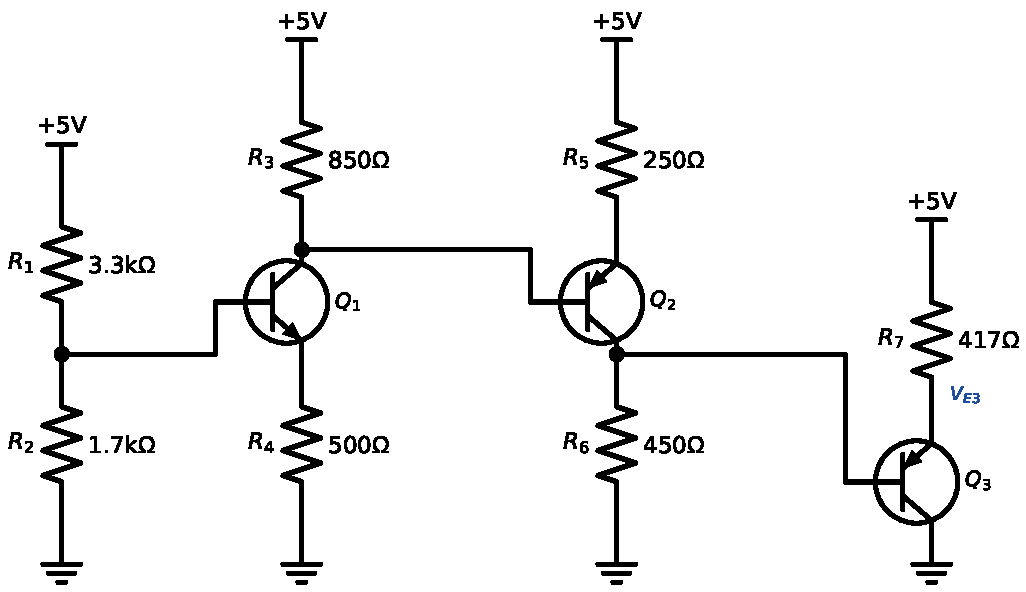
\includegraphics[width=0.85\linewidth,height=6cm,keepaspectratio]{p13_designed}\end{center}

\solstep{4}{Check the design}\begin{itemize}[leftmargin=*,itemsep=2pt]
\item $I_{B1} = \frac{I_{C1}}{\beta} = 20\,\mu \mathrm{A}$ $\ll$ the $1\,\mathrm{m}\mathrm{A}$ flowing in the base network \checkmark
\item $I_{B2} = \frac{I_{C2}}{\beta} = 40\,\mu \mathrm{A}$ $\ll$ the $2\,\mathrm{m}\mathrm{A}$ flowing in the base network \checkmark
\item $I_{B3} = \frac{I_{C3}}{\beta} = 60\,\mu \mathrm{A}$ $\ll$ the $4\,\mathrm{m}\mathrm{A}$ flowing in the base network \checkmark
\item $V_{CE1} = V_{C1} - V_{E1} = 3.3 - 1 = 2.3\,\mathrm{V} \ge 1$\,V \checkmark
\item $V_{EC2} = V_{E2} - V_{C2} = 4 - 1.8 = 2.2\,\mathrm{V} \ge 1$\,V \checkmark
\item $V_{EC3} = V_{E3} - 0 = 2.5 - 0 = 2.5\,\mathrm{V} \ge 1$\,V \checkmark
\item $I_{dc} = I_{R1} + I_{R3} + I_{R5} + I_{R7} = 1\,\mathrm{m}\mathrm{A} + 2\,\mathrm{m}\mathrm{A} + 4\,\mathrm{m}\mathrm{A} + 6\,\mathrm{m}\mathrm{A} = 13\,\mathrm{m}\mathrm{A} \le 14\,\mathrm{m}\mathrm{A}$ \checkmark
\end{itemize}
Finally the designed circuit is solved exactly ($\beta=100$, base currents included), once with $|V_{BE}|=0.7$\,V and once with each transistor's $|V_{BE}|$ changed to $0.6$ and $0.8$\,V:\begin{center}\renewcommand{\arraystretch}{1.35}
\begin{tabular}{cccccc}
\toprule
 & target $I_C$ & exact $I_C$ & $|V_{BE}|=0.6$ & $|V_{BE}|=0.8$ & max change \\
\midrule
$Q_{1}$ & $2\,\mathrm{m}\mathrm{A}$ & $1.94\,\mathrm{m}\mathrm{A}$ & $2.13\,\mathrm{m}\mathrm{A}$ & $1.74\,\mathrm{m}\mathrm{A}$ & $9.7\,\%$ \\
$Q_{2}$ & $4\,\mathrm{m}\mathrm{A}$ & $3.63\,\mathrm{m}\mathrm{A}$ & $4.01\,\mathrm{m}\mathrm{A}$ & $3.24\,\mathrm{m}\mathrm{A}$ & $9.6\,\%$ \\
$Q_{3}$ & $6\,\mathrm{m}\mathrm{A}$ & $6.27\,\mathrm{m}\mathrm{A}$ & $6.51\,\mathrm{m}\mathrm{A}$ & $6.04\,\mathrm{m}\mathrm{A}$ & $3.9\,\%$ \\
\bottomrule
\end{tabular}\end{center}
A $\pm0.1$\,V change of $V_{BE}$ moves no current by more than about $10\,\%$ of its design value ($V_{BE}$-insensitive), and the exact currents are close to the targets ($I_B$ negligible). The exact currents drift further from the targets along a chain of direct-coupled stages: each base current and each $I_C = \alpha I_E$ slightly shifts the collector voltage that biases the next stage, and with only $\approx1$\,V across the next emitter resistor that shift is amplified. This is the normal accuracy of a hand design with $I_B\approx0$; a larger emitter-resistor voltage in the later stages reduces the drift.
\begin{ansbox}
$R_{1} = 3.3\,\mathrm{k}\Omega$,\quad $R_{2} = 1.7\,\mathrm{k}\Omega$,\quad $R_{3} = 850\,\Omega$,\quad $R_{4} = 500\,\Omega$,\quad $R_{5} = 250\,\Omega$,\quad $R_{6} = 450\,\Omega$,\quad $R_{7} = 417\,\Omega$
\end{ansbox}

\newpage
\subsection*{Solution 4C.14 \hfill Hard}
\begin{center}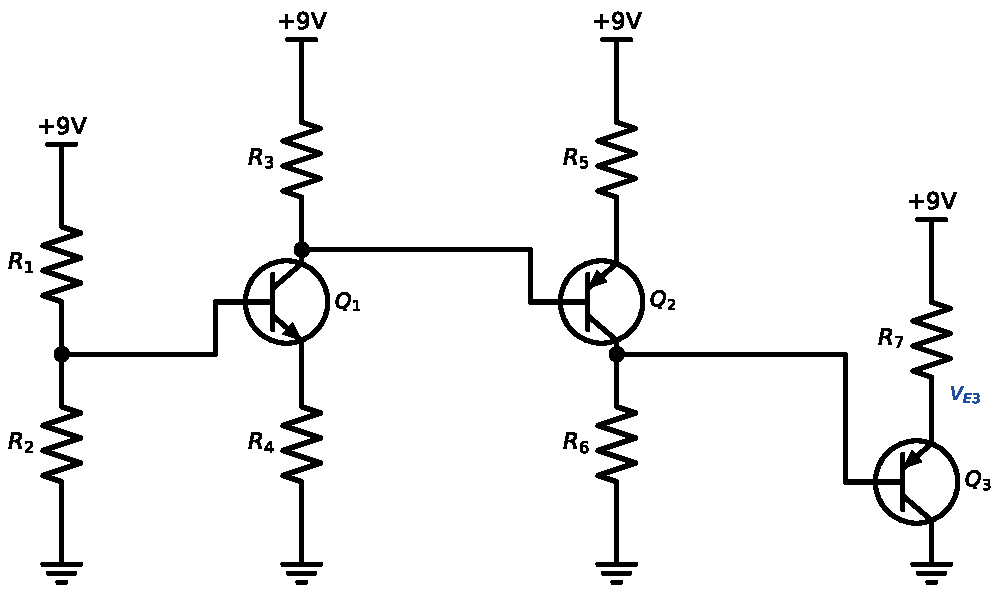
\includegraphics[width=0.9\linewidth,height=6cm,keepaspectratio]{p14_circuit}\end{center}
\solstep{1}{Rules}With $I_B\approx0$ and every transistor active ($|V_{BE}|=0.7$\,V, $I_C\approx I_E$), a resistor is known as soon as the voltages at both of its ends and the current through it are known: $R = \Delta V / I$. The specifications give the currents and some node voltages; the remaining freedom is removed with two rules:\begin{itemize}[leftmargin=*,itemsep=1pt]
\item $V_{BE}$-insensitive: the voltage across the resistor that sets an emitter current must be at least $1$\,V (then $\pm0.1$\,V of $V_{BE}$ changes $I_C$ by at most $10\,\%$);
\item $\beta$-insensitive: a divider current must be much larger ($\ge 10\times$) than the base current it feeds, and a collector current that drives a base must be much larger than that base current.
\end{itemize}
Work from the nodes that are already fixed towards the unknown ones.
\solstep{2}{Design, node by node}\begin{enumerate}[leftmargin=*,itemsep=3pt]
\item $V_{BE}$-insensitivity: a $0.1$\,V change of $V_{BE}$ changes the voltage across $R_{5}$ by $0.1$\,V, so $\frac{\Delta I_C}{I_C} = \frac{0.1}{V_{R5}} \le 10\%$ needs $V_{R5} \ge 1$\,V. Choose the smallest value, $V_{R5} = 1$\,V: $V_{E2} = 9 - V_{R5} = 9 - 1 = 8\,\mathrm{V}$.
\item $V_{BE}$-insensitivity: a $0.1$\,V change of $V_{BE}$ changes the voltage across $R_{4}$ by $0.1$\,V, so $\frac{\Delta I_C}{I_C} = \frac{0.1}{V_{R4}} \le 10\%$ needs $V_{R4} \ge 1$\,V. Choose the smallest value, $V_{R4} = 1$\,V: $V_{E1} = 0 + V_{R4} = 0 + 1 = 1\,\mathrm{V}$.
\item $I_{dc} = I_{R1} + I_{C1} + I_{C2} + I_{C3} \le 9\,\mathrm{mA}$ leaves at most $9 - 1 - 2 - 5 = 1\,\mathrm{mA}$ for the divider, and $I_{R2}$ must be $\gg I_{B1} = 10\,\mu\mathrm{A}$. Choose $I_{R2} = 0.5\,\mathrm{mA}$.
\item $Q_{1}$ is active: $V_{B1} = V_{E1} + 0.7 = 1.7\,\mathrm{V}$.
\item $Q_{2}$ is active: $V_{C1} = V_{E2} - 0.7 = 7.3\,\mathrm{V}$.
\item $Q_{3}$ is active: $V_{C2} = V_{E3} - 0.7 = 4.3\,\mathrm{V}$.
\item With $I_B\approx0$ the only current through $R_{1}$ is $I_{R2}$: $I_{R1} = I_{R2} = 500\,\mu \mathrm{A}$.
\item $\displaystyle R_{1} = \frac{9 - V_{B1}}{I_{R2}} = \frac{9 - 1.7}{500\,\mu \mathrm{A}} = \mathbf{14.6\,\mathrm{k}\Omega}$
\item $\displaystyle R_{2} = \frac{V_{B1} - 0}{I_{R2}} = \frac{1.7 - 0}{500\,\mu \mathrm{A}} = \mathbf{3.4\,\mathrm{k}\Omega}$
\item With $I_B\approx0$ the only current through $R_{3}$ is $I_{C1}$: $I_{R3} = I_{C1} = 1\,\mathrm{m}\mathrm{A}$.
\item $\displaystyle R_{3} = \frac{9 - V_{C1}}{I_{C1}} = \frac{9 - 7.3}{1\,\mathrm{m}\mathrm{A}} = \mathbf{1.7\,\mathrm{k}\Omega}$
\item With $I_B\approx0$ the only current through $R_{4}$ is $I_{E1}$: $I_{R4} = I_{E1} = 1\,\mathrm{m}\mathrm{A}$ ($I_C\approx I_E$).
\item $\displaystyle R_{4} = \frac{V_{E1} - 0}{I_{E1}} = \frac{1 - 0}{1\,\mathrm{m}\mathrm{A}} = \mathbf{1\,\mathrm{k}\Omega}$
\item With $I_B\approx0$ the only current through $R_{5}$ is $I_{E2}$: $I_{R5} = I_{E2} = 2\,\mathrm{m}\mathrm{A}$ ($I_C\approx I_E$).
\item $\displaystyle R_{5} = \frac{9 - V_{E2}}{I_{E2}} = \frac{9 - 8}{2\,\mathrm{m}\mathrm{A}} = \mathbf{500\,\Omega}$
\item With $I_B\approx0$ the only current through $R_{6}$ is $I_{C2}$: $I_{R6} = I_{C2} = 2\,\mathrm{m}\mathrm{A}$.
\item $\displaystyle R_{6} = \frac{V_{C2} - 0}{I_{C2}} = \frac{4.3 - 0}{2\,\mathrm{m}\mathrm{A}} = \mathbf{2.15\,\mathrm{k}\Omega}$
\item With $I_B\approx0$ the only current through $R_{7}$ is $I_{E3}$: $I_{R7} = I_{E3} = 5\,\mathrm{m}\mathrm{A}$ ($I_C\approx I_E$).
\item $\displaystyle R_{7} = \frac{9 - V_{E3}}{I_{E3}} = \frac{9 - 5}{5\,\mathrm{m}\mathrm{A}} = \mathbf{800\,\Omega}$
\end{enumerate}

\solstep{3}{Designed circuit}\begin{center}\renewcommand{\arraystretch}{1.35}
\begin{tabular}{cc}
\toprule
resistor & value \\
\midrule
$R_{1}$ & $14.6\,\mathrm{k}\Omega$ \\
$R_{2}$ & $3.4\,\mathrm{k}\Omega$ \\
$R_{3}$ & $1.7\,\mathrm{k}\Omega$ \\
$R_{4}$ & $1\,\mathrm{k}\Omega$ \\
$R_{5}$ & $500\,\Omega$ \\
$R_{6}$ & $2.15\,\mathrm{k}\Omega$ \\
$R_{7}$ & $800\,\Omega$ \\
\bottomrule
\end{tabular}\end{center}
\begin{center}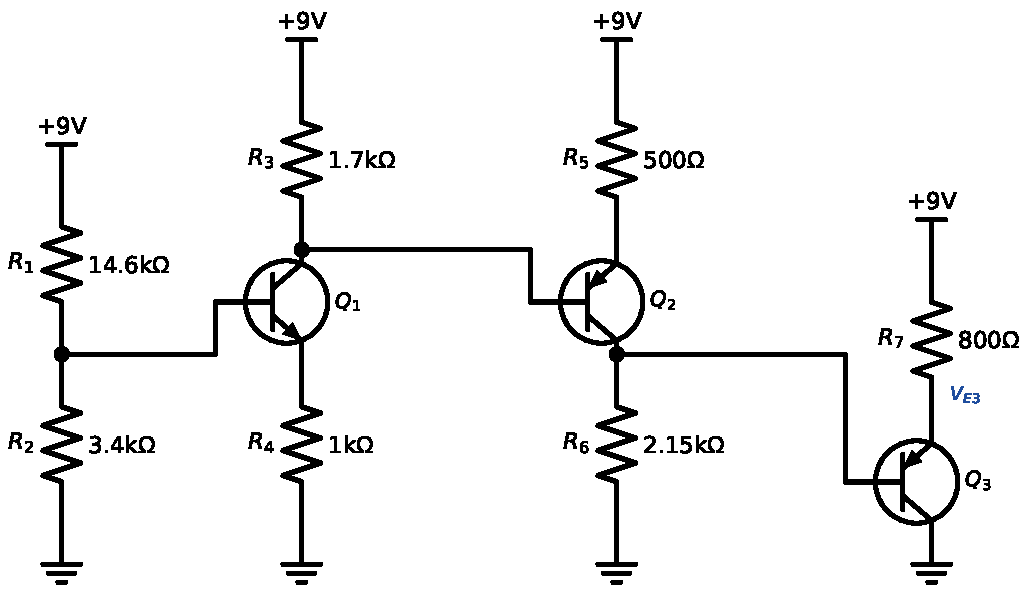
\includegraphics[width=0.85\linewidth,height=6cm,keepaspectratio]{p14_designed}\end{center}

\solstep{4}{Check the design}\begin{itemize}[leftmargin=*,itemsep=2pt]
\item $I_{B1} = \frac{I_{C1}}{\beta} = 10\,\mu \mathrm{A}$ $\ll$ the $500\,\mu \mathrm{A}$ flowing in the base network \checkmark
\item $I_{B2} = \frac{I_{C2}}{\beta} = 20\,\mu \mathrm{A}$ $\ll$ the $1\,\mathrm{m}\mathrm{A}$ flowing in the base network \checkmark
\item $I_{B3} = \frac{I_{C3}}{\beta} = 50\,\mu \mathrm{A}$ $\ll$ the $2\,\mathrm{m}\mathrm{A}$ flowing in the base network \checkmark
\item $V_{CE1} = V_{C1} - V_{E1} = 7.3 - 1 = 6.3\,\mathrm{V} \ge 1$\,V \checkmark
\item $V_{EC2} = V_{E2} - V_{C2} = 8 - 4.3 = 3.7\,\mathrm{V} \ge 1$\,V \checkmark
\item $V_{EC3} = V_{E3} - 0 = 5 - 0 = 5\,\mathrm{V} \ge 1$\,V \checkmark
\item $I_{dc} = I_{R1} + I_{R3} + I_{R5} + I_{R7} = 500\,\mu \mathrm{A} + 1\,\mathrm{m}\mathrm{A} + 2\,\mathrm{m}\mathrm{A} + 5\,\mathrm{m}\mathrm{A} = 8.5\,\mathrm{m}\mathrm{A} \le 9\,\mathrm{m}\mathrm{A}$ \checkmark
\end{itemize}
Finally the designed circuit is solved exactly ($\beta=100$, base currents included), once with $|V_{BE}|=0.7$\,V and once with each transistor's $|V_{BE}|$ changed to $0.6$ and $0.8$\,V:\begin{center}\renewcommand{\arraystretch}{1.35}
\begin{tabular}{cccccc}
\toprule
 & target $I_C$ & exact $I_C$ & $|V_{BE}|=0.6$ & $|V_{BE}|=0.8$ & max change \\
\midrule
$Q_{1}$ & $1\,\mathrm{m}\mathrm{A}$ & $964\,\mu \mathrm{A}$ & $1.06\,\mathrm{m}\mathrm{A}$ & $867\,\mu \mathrm{A}$ & $9.6\,\%$ \\
$Q_{2}$ & $2\,\mathrm{m}\mathrm{A}$ & $1.8\,\mathrm{m}\mathrm{A}$ & $1.99\,\mathrm{m}\mathrm{A}$ & $1.61\,\mathrm{m}\mathrm{A}$ & $9.6\,\%$ \\
$Q_{3}$ & $5\,\mathrm{m}\mathrm{A}$ & $5.35\,\mathrm{m}\mathrm{A}$ & $5.47\,\mathrm{m}\mathrm{A}$ & $5.23\,\mathrm{m}\mathrm{A}$ & $2.4\,\%$ \\
\bottomrule
\end{tabular}\end{center}
A $\pm0.1$\,V change of $V_{BE}$ moves no current by more than about $10\,\%$ of its design value ($V_{BE}$-insensitive), and the exact currents are close to the targets ($I_B$ negligible). The exact currents drift further from the targets along a chain of direct-coupled stages: each base current and each $I_C = \alpha I_E$ slightly shifts the collector voltage that biases the next stage, and with only $\approx1$\,V across the next emitter resistor that shift is amplified. This is the normal accuracy of a hand design with $I_B\approx0$; a larger emitter-resistor voltage in the later stages reduces the drift.
\begin{ansbox}
$R_{1} = 14.6\,\mathrm{k}\Omega$,\quad $R_{2} = 3.4\,\mathrm{k}\Omega$,\quad $R_{3} = 1.7\,\mathrm{k}\Omega$,\quad $R_{4} = 1\,\mathrm{k}\Omega$,\quad $R_{5} = 500\,\Omega$,\quad $R_{6} = 2.15\,\mathrm{k}\Omega$,\quad $R_{7} = 800\,\Omega$
\end{ansbox}

\newpage
\subsection*{Solution 4C.15 \hfill Hard}
\begin{center}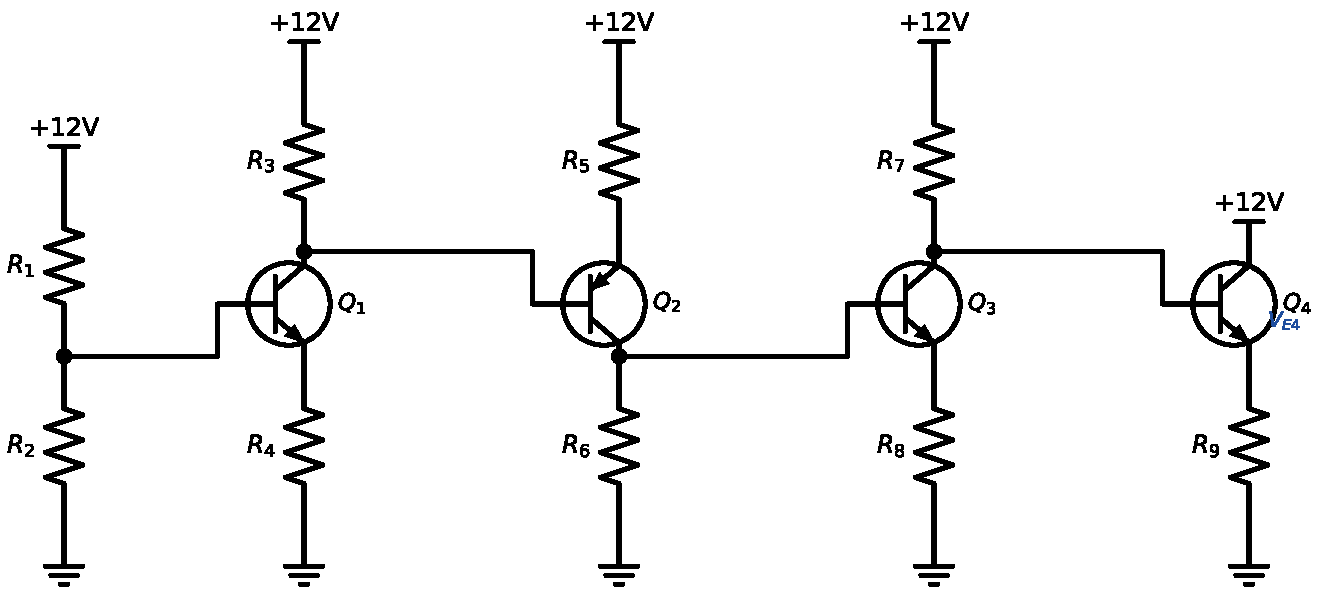
\includegraphics[width=0.9\linewidth,height=6cm,keepaspectratio]{p15_circuit}\end{center}
\solstep{1}{Rules}With $I_B\approx0$ and every transistor active ($|V_{BE}|=0.7$\,V, $I_C\approx I_E$), a resistor is known as soon as the voltages at both of its ends and the current through it are known: $R = \Delta V / I$. The specifications give the currents and some node voltages; the remaining freedom is removed with two rules:\begin{itemize}[leftmargin=*,itemsep=1pt]
\item $V_{BE}$-insensitive: the voltage across the resistor that sets an emitter current must be at least $1$\,V (then $\pm0.1$\,V of $V_{BE}$ changes $I_C$ by at most $10\,\%$);
\item $\beta$-insensitive: a divider current must be much larger ($\ge 10\times$) than the base current it feeds, and a collector current that drives a base must be much larger than that base current.
\end{itemize}
Work from the nodes that are already fixed towards the unknown ones.
\solstep{2}{Design, node by node}\begin{enumerate}[leftmargin=*,itemsep=3pt]
\item $V_{BE}$-insensitivity: a $0.1$\,V change of $V_{BE}$ changes the voltage across $R_{4}$ by $0.1$\,V, so $\frac{\Delta I_C}{I_C} = \frac{0.1}{V_{R4}} \le 10\%$ needs $V_{R4} \ge 1$\,V. Choose the smallest value, $V_{R4} = 1$\,V: $V_{E1} = 0 + V_{R4} = 0 + 1 = 1\,\mathrm{V}$.
\item $V_{BE}$-insensitivity: a $0.1$\,V change of $V_{BE}$ changes the voltage across $R_{5}$ by $0.1$\,V, so $\frac{\Delta I_C}{I_C} = \frac{0.1}{V_{R5}} \le 10\%$ needs $V_{R5} \ge 1$\,V. As specified (larger, for accuracy), $V_{R5} = 2$\,V: $V_{E2} = 12 - V_{R5} = 12 - 2 = 10\,\mathrm{V}$.
\item $V_{BE}$-insensitivity: a $0.1$\,V change of $V_{BE}$ changes the voltage across $R_{8}$ by $0.1$\,V, so $\frac{\Delta I_C}{I_C} = \frac{0.1}{V_{R8}} \le 10\%$ needs $V_{R8} \ge 1$\,V. As specified (larger, for accuracy), $V_{R8} = 2$\,V: $V_{E3} = 0 + V_{R8} = 0 + 2 = 2\,\mathrm{V}$.
\item The divider current must be much larger than the base current it feeds ($I_{B1} = 10\,\mu \mathrm{A}$). Choose $I_{R2} = 500\,\mu \mathrm{A}$ (50 times larger).
\item $Q_{1}$ is active: $V_{B1} = V_{E1} + 0.7 = 1.7\,\mathrm{V}$.
\item $Q_{2}$ is active: $V_{C1} = V_{E2} - 0.7 = 9.3\,\mathrm{V}$.
\item $Q_{3}$ is active: $V_{C2} = V_{E3} + 0.7 = 2.7\,\mathrm{V}$.
\item $Q_{4}$ is active: $V_{C3} = V_{E4} + 0.7 = 6.7\,\mathrm{V}$.
\item With $I_B\approx0$ the only current through $R_{1}$ is $I_{R2}$: $I_{R1} = I_{R2} = 500\,\mu \mathrm{A}$.
\item $\displaystyle R_{1} = \frac{12 - V_{B1}}{I_{R2}} = \frac{12 - 1.7}{500\,\mu \mathrm{A}} = \mathbf{20.6\,\mathrm{k}\Omega}$
\item $\displaystyle R_{2} = \frac{V_{B1} - 0}{I_{R2}} = \frac{1.7 - 0}{500\,\mu \mathrm{A}} = \mathbf{3.4\,\mathrm{k}\Omega}$
\item With $I_B\approx0$ the only current through $R_{3}$ is $I_{C1}$: $I_{R3} = I_{C1} = 1\,\mathrm{m}\mathrm{A}$.
\item $\displaystyle R_{3} = \frac{12 - V_{C1}}{I_{C1}} = \frac{12 - 9.3}{1\,\mathrm{m}\mathrm{A}} = \mathbf{2.7\,\mathrm{k}\Omega}$
\item With $I_B\approx0$ the only current through $R_{4}$ is $I_{E1}$: $I_{R4} = I_{E1} = 1\,\mathrm{m}\mathrm{A}$ ($I_C\approx I_E$).
\item $\displaystyle R_{4} = \frac{V_{E1} - 0}{I_{E1}} = \frac{1 - 0}{1\,\mathrm{m}\mathrm{A}} = \mathbf{1\,\mathrm{k}\Omega}$
\item With $I_B\approx0$ the only current through $R_{5}$ is $I_{E2}$: $I_{R5} = I_{E2} = 2\,\mathrm{m}\mathrm{A}$ ($I_C\approx I_E$).
\item $\displaystyle R_{5} = \frac{12 - V_{E2}}{I_{E2}} = \frac{12 - 10}{2\,\mathrm{m}\mathrm{A}} = \mathbf{1\,\mathrm{k}\Omega}$
\item With $I_B\approx0$ the only current through $R_{6}$ is $I_{C2}$: $I_{R6} = I_{C2} = 2\,\mathrm{m}\mathrm{A}$.
\item $\displaystyle R_{6} = \frac{V_{C2} - 0}{I_{C2}} = \frac{2.7 - 0}{2\,\mathrm{m}\mathrm{A}} = \mathbf{1.35\,\mathrm{k}\Omega}$
\item With $I_B\approx0$ the only current through $R_{7}$ is $I_{C3}$: $I_{R7} = I_{C3} = 2\,\mathrm{m}\mathrm{A}$.
\item $\displaystyle R_{7} = \frac{12 - V_{C3}}{I_{C3}} = \frac{12 - 6.7}{2\,\mathrm{m}\mathrm{A}} = \mathbf{2.65\,\mathrm{k}\Omega}$
\item With $I_B\approx0$ the only current through $R_{8}$ is $I_{E3}$: $I_{R8} = I_{E3} = 2\,\mathrm{m}\mathrm{A}$ ($I_C\approx I_E$).
\item $\displaystyle R_{8} = \frac{V_{E3} - 0}{I_{E3}} = \frac{2 - 0}{2\,\mathrm{m}\mathrm{A}} = \mathbf{1\,\mathrm{k}\Omega}$
\item With $I_B\approx0$ the only current through $R_{9}$ is $I_{E4}$: $I_{R9} = I_{E4} = 5\,\mathrm{m}\mathrm{A}$ ($I_C\approx I_E$).
\item $\displaystyle R_{9} = \frac{V_{E4} - 0}{I_{E4}} = \frac{6 - 0}{5\,\mathrm{m}\mathrm{A}} = \mathbf{1.2\,\mathrm{k}\Omega}$
\end{enumerate}

\solstep{3}{Designed circuit}\begin{center}\renewcommand{\arraystretch}{1.35}
\begin{tabular}{cc}
\toprule
resistor & value \\
\midrule
$R_{1}$ & $20.6\,\mathrm{k}\Omega$ \\
$R_{2}$ & $3.4\,\mathrm{k}\Omega$ \\
$R_{3}$ & $2.7\,\mathrm{k}\Omega$ \\
$R_{4}$ & $1\,\mathrm{k}\Omega$ \\
$R_{5}$ & $1\,\mathrm{k}\Omega$ \\
$R_{6}$ & $1.35\,\mathrm{k}\Omega$ \\
$R_{7}$ & $2.65\,\mathrm{k}\Omega$ \\
$R_{8}$ & $1\,\mathrm{k}\Omega$ \\
$R_{9}$ & $1.2\,\mathrm{k}\Omega$ \\
\bottomrule
\end{tabular}\end{center}
\begin{center}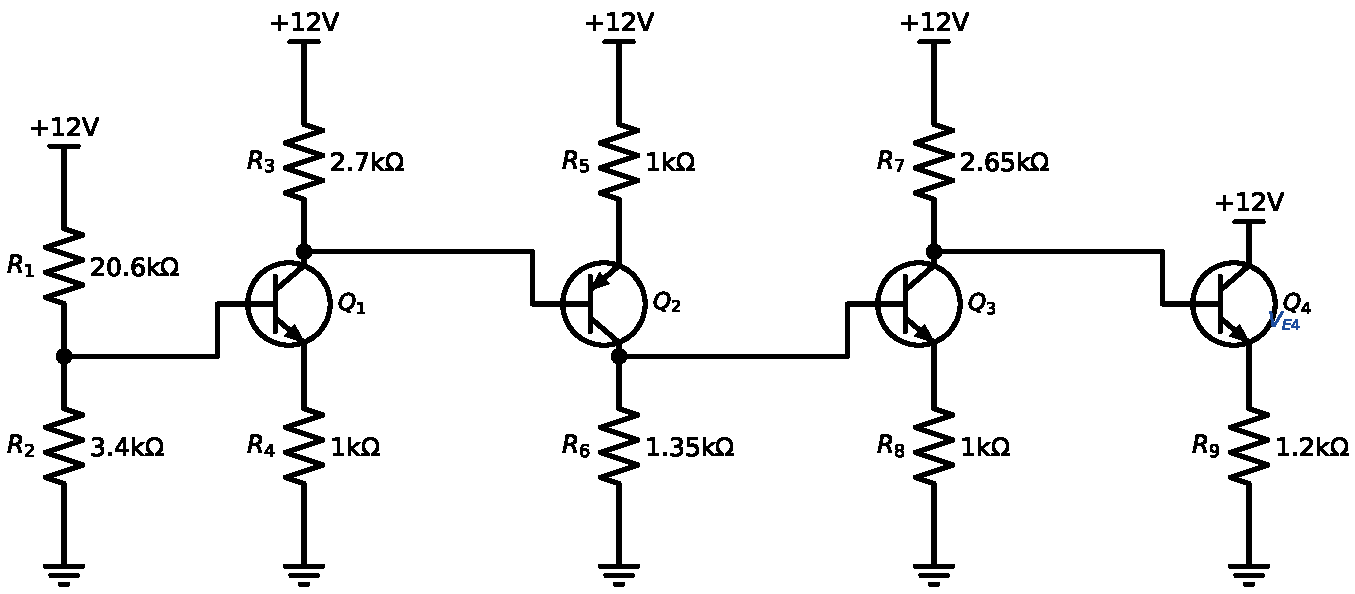
\includegraphics[width=0.85\linewidth,height=6cm,keepaspectratio]{p15_designed}\end{center}

\solstep{4}{Check the design}\begin{itemize}[leftmargin=*,itemsep=2pt]
\item $I_{B1} = \frac{I_{C1}}{\beta} = 10\,\mu \mathrm{A}$ $\ll$ the $500\,\mu \mathrm{A}$ flowing in the base network \checkmark
\item $I_{B2} = \frac{I_{C2}}{\beta} = 20\,\mu \mathrm{A}$ $\ll$ the $1\,\mathrm{m}\mathrm{A}$ flowing in the base network \checkmark
\item $I_{B3} = \frac{I_{C3}}{\beta} = 20\,\mu \mathrm{A}$ $\ll$ the $2\,\mathrm{m}\mathrm{A}$ flowing in the base network \checkmark
\item $I_{B4} = \frac{I_{C4}}{\beta} = 50\,\mu \mathrm{A}$ $\ll$ the $2\,\mathrm{m}\mathrm{A}$ flowing in the base network \checkmark
\item $V_{CE1} = V_{C1} - V_{E1} = 9.3 - 1 = 8.3\,\mathrm{V} \ge 1$\,V \checkmark
\item $V_{EC2} = V_{E2} - V_{C2} = 10 - 2.7 = 7.3\,\mathrm{V} \ge 1$\,V \checkmark
\item $V_{CE3} = V_{C3} - V_{E3} = 6.7 - 2 = 4.7\,\mathrm{V} \ge 1$\,V \checkmark
\item $V_{CE4} = 12 - V_{E4} = 12 - 6 = 6\,\mathrm{V} \ge 1$\,V \checkmark
\end{itemize}
Finally the designed circuit is solved exactly ($\beta=100$, base currents included), once with $|V_{BE}|=0.7$\,V and once with each transistor's $|V_{BE}|$ changed to $0.6$ and $0.8$\,V:\begin{center}\renewcommand{\arraystretch}{1.35}
\begin{tabular}{cccccc}
\toprule
 & target $I_C$ & exact $I_C$ & $|V_{BE}|=0.6$ & $|V_{BE}|=0.8$ & max change \\
\midrule
$Q_{1}$ & $1\,\mathrm{m}\mathrm{A}$ & $962\,\mu \mathrm{A}$ & $1.06\,\mathrm{m}\mathrm{A}$ & $866\,\mu \mathrm{A}$ & $9.6\,\%$ \\
$Q_{2}$ & $2\,\mathrm{m}\mathrm{A}$ & $1.83\,\mathrm{m}\mathrm{A}$ & $1.93\,\mathrm{m}\mathrm{A}$ & $1.73\,\mathrm{m}\mathrm{A}$ & $4.8\,\%$ \\
$Q_{3}$ & $2\,\mathrm{m}\mathrm{A}$ & $1.73\,\mathrm{m}\mathrm{A}$ & $1.83\,\mathrm{m}\mathrm{A}$ & $1.63\,\mathrm{m}\mathrm{A}$ & $4.9\,\%$ \\
$Q_{4}$ & $5\,\mathrm{m}\mathrm{A}$ & $5.42\,\mathrm{m}\mathrm{A}$ & $5.5\,\mathrm{m}\mathrm{A}$ & $5.34\,\mathrm{m}\mathrm{A}$ & $1.6\,\%$ \\
\bottomrule
\end{tabular}\end{center}
A $\pm0.1$\,V change of $V_{BE}$ moves no current by more than about $10\,\%$ of its design value ($V_{BE}$-insensitive), and the exact currents are close to the targets ($I_B$ negligible). The exact currents drift further from the targets along a chain of direct-coupled stages: each base current and each $I_C = \alpha I_E$ slightly shifts the collector voltage that biases the next stage, and with only $\approx1$\,V across the next emitter resistor that shift is amplified. This is the normal accuracy of a hand design with $I_B\approx0$; a larger emitter-resistor voltage in the later stages reduces the drift.
\begin{ansbox}
$R_{1} = 20.6\,\mathrm{k}\Omega$,\quad $R_{2} = 3.4\,\mathrm{k}\Omega$,\quad $R_{3} = 2.7\,\mathrm{k}\Omega$,\quad $R_{4} = 1\,\mathrm{k}\Omega$,\quad $R_{5} = 1\,\mathrm{k}\Omega$,\quad $R_{6} = 1.35\,\mathrm{k}\Omega$,\quad $R_{7} = 2.65\,\mathrm{k}\Omega$,\quad $R_{8} = 1\,\mathrm{k}\Omega$,\quad $R_{9} = 1.2\,\mathrm{k}\Omega$
\end{ansbox}

\newpage
\subsection*{Solution 4C.16 \hfill Hard}
\begin{center}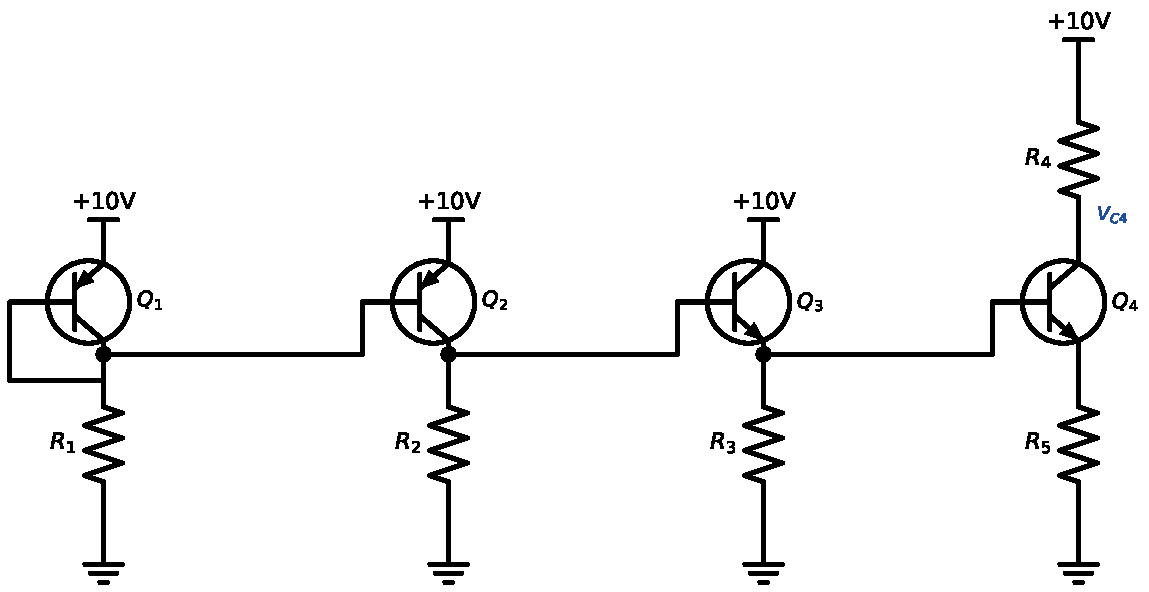
\includegraphics[width=0.9\linewidth,height=6cm,keepaspectratio]{p16_circuit}\end{center}
\solstep{1}{Rules}With $I_B\approx0$ and every transistor active ($|V_{BE}|=0.7$\,V, $I_C\approx I_E$), a resistor is known as soon as the voltages at both of its ends and the current through it are known: $R = \Delta V / I$. The specifications give the currents and some node voltages; the remaining freedom is removed with two rules:\begin{itemize}[leftmargin=*,itemsep=1pt]
\item $V_{BE}$-insensitive: the voltage across the resistor that sets an emitter current must be at least $1$\,V (then $\pm0.1$\,V of $V_{BE}$ changes $I_C$ by at most $10\,\%$);
\item $\beta$-insensitive: a divider current must be much larger ($\ge 10\times$) than the base current it feeds, and a collector current that drives a base must be much larger than that base current.
\end{itemize}
Work from the nodes that are already fixed towards the unknown ones.
\solstep{2}{Design, node by node}\begin{enumerate}[leftmargin=*,itemsep=3pt]
\item $Q_{1}$ (diode-connected) is active: $V_{B1} = 10 - 0.7 = 9.3\,\mathrm{V}$.
\item $Q_{3}$ is active: $V_{C2} = V_{E3} + 0.7 = 4.7\,\mathrm{V}$.
\item $Q_{4}$ is active: $V_{E4} = V_{E3} - 0.7 = 3.3\,\mathrm{V}$.
\item $Q_{2}$ mirrors $Q_{1}$ (same base and emitter nodes): $I_{C2} = I_{C1} = 2\,\mathrm{m}\mathrm{A}$.
\item With $I_B\approx0$ the only current through $R_{1}$ is $I_{C1}$: $I_{R1} = I_{C1} = 2\,\mathrm{m}\mathrm{A}$.
\item $\displaystyle R_{1} = \frac{V_{B1} - 0}{I_{C1}} = \frac{9.3 - 0}{2\,\mathrm{m}\mathrm{A}} = \mathbf{4.65\,\mathrm{k}\Omega}$
\item With $I_B\approx0$ the only current through $R_{2}$ is $I_{C2}$: $I_{R2} = I_{C2} = 2\,\mathrm{m}\mathrm{A}$.
\item $\displaystyle R_{2} = \frac{V_{C2} - 0}{I_{C2}} = \frac{4.7 - 0}{2\,\mathrm{m}\mathrm{A}} = \mathbf{2.35\,\mathrm{k}\Omega}$
\item With $I_B\approx0$ the only current through $R_{3}$ is $I_{E3}$: $I_{R3} = I_{E3} = 4\,\mathrm{m}\mathrm{A}$ ($I_C\approx I_E$).
\item $\displaystyle R_{3} = \frac{V_{E3} - 0}{I_{E3}} = \frac{4 - 0}{4\,\mathrm{m}\mathrm{A}} = \mathbf{1\,\mathrm{k}\Omega}$
\item With $I_B\approx0$ the only current through $R_{4}$ is $I_{C4}$: $I_{R4} = I_{C4} = 1\,\mathrm{m}\mathrm{A}$.
\item $\displaystyle R_{4} = \frac{10 - V_{C4}}{I_{C4}} = \frac{10 - 7}{1\,\mathrm{m}\mathrm{A}} = \mathbf{3\,\mathrm{k}\Omega}$
\item With $I_B\approx0$ the only current through $R_{5}$ is $I_{E4}$: $I_{R5} = I_{E4} = 1\,\mathrm{m}\mathrm{A}$ ($I_C\approx I_E$).
\item $\displaystyle R_{5} = \frac{V_{E4} - 0}{I_{E4}} = \frac{3.3 - 0}{1\,\mathrm{m}\mathrm{A}} = \mathbf{3.3\,\mathrm{k}\Omega}$
\end{enumerate}

\solstep{3}{Designed circuit}\begin{center}\renewcommand{\arraystretch}{1.35}
\begin{tabular}{cc}
\toprule
resistor & value \\
\midrule
$R_{1}$ & $4.65\,\mathrm{k}\Omega$ \\
$R_{2}$ & $2.35\,\mathrm{k}\Omega$ \\
$R_{3}$ & $1\,\mathrm{k}\Omega$ \\
$R_{4}$ & $3\,\mathrm{k}\Omega$ \\
$R_{5}$ & $3.3\,\mathrm{k}\Omega$ \\
\bottomrule
\end{tabular}\end{center}
\begin{center}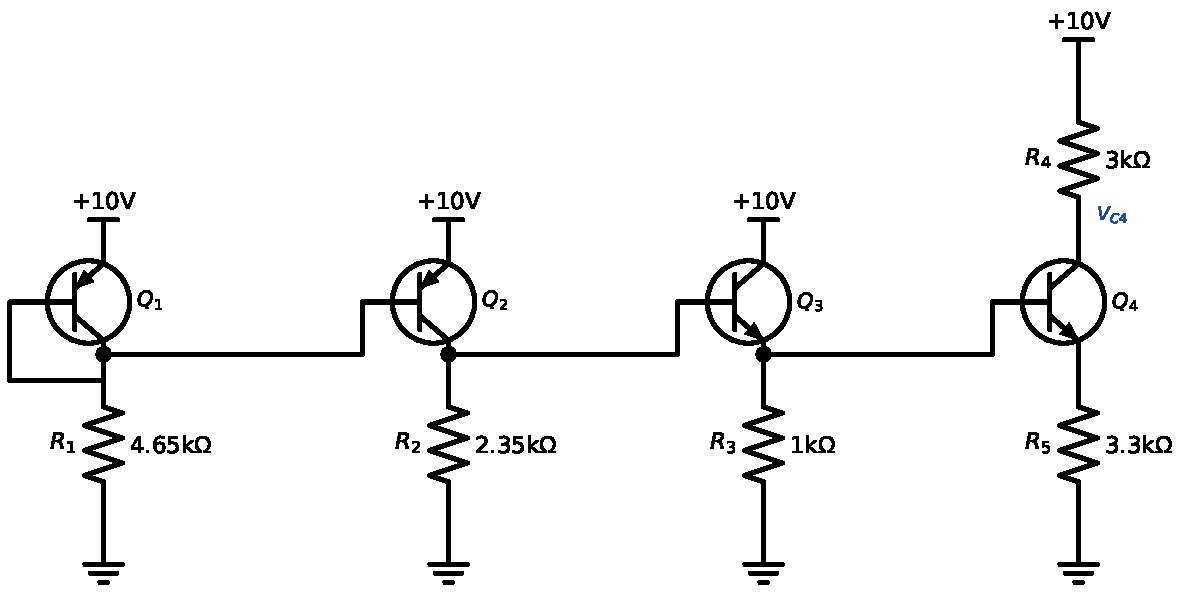
\includegraphics[width=0.85\linewidth,height=6cm,keepaspectratio]{p16_designed}\end{center}

\solstep{4}{Check the design}\begin{itemize}[leftmargin=*,itemsep=2pt]
\item $I_{B1} = \frac{I_{C1}}{\beta} = 20\,\mu \mathrm{A}$ (all bases on this node: $40\,\mu \mathrm{A}$) $\ll$ the $2\,\mathrm{m}\mathrm{A}$ flowing in the base network \checkmark
\item $I_{B2} = \frac{I_{C2}}{\beta} = 20\,\mu \mathrm{A}$ (all bases on this node: $40\,\mu \mathrm{A}$) $\ll$ the $2\,\mathrm{m}\mathrm{A}$ flowing in the base network \checkmark
\item $I_{B3} = \frac{I_{C3}}{\beta} = 40\,\mu \mathrm{A}$ $\ll$ the $2\,\mathrm{m}\mathrm{A}$ flowing in the base network \checkmark
\item $I_{B4} = \frac{I_{C4}}{\beta} = 10\,\mu \mathrm{A}$ $\ll$ the $4\,\mathrm{m}\mathrm{A}$ flowing in the base network \checkmark
\item $Q_{1}$ is diode-connected: $V_{EC1} = |V_{BE}| = 0.7$\,V, always active (the $|V_{CE}|$ specification is meant for the other transistors) \checkmark
\item $V_{EC2} = 10 - V_{C2} = 10 - 4.7 = 5.3\,\mathrm{V} \ge 1$\,V \checkmark
\item $V_{CE3} = 10 - V_{E3} = 10 - 4 = 6\,\mathrm{V} \ge 1$\,V \checkmark
\item $V_{CE4} = V_{C4} - V_{E4} = 7 - 3.3 = 3.7\,\mathrm{V} \ge 1$\,V \checkmark
\item $I_{dc} = I_{R4} + I_{C1} + I_{C2} + I_{C3} = 1\,\mathrm{m}\mathrm{A} + 2\,\mathrm{m}\mathrm{A} + 2\,\mathrm{m}\mathrm{A} + 4\,\mathrm{m}\mathrm{A} = 9\,\mathrm{m}\mathrm{A} \le 10\,\mathrm{m}\mathrm{A}$ \checkmark
\end{itemize}
Finally the designed circuit is solved exactly ($\beta=100$, base currents included), once with $|V_{BE}|=0.7$\,V and once with each transistor's $|V_{BE}|$ changed to $0.6$ and $0.8$\,V:\begin{center}\renewcommand{\arraystretch}{1.35}
\begin{tabular}{cccccc}
\toprule
 & target $I_C$ & exact $I_C$ & $|V_{BE}|=0.6$ & $|V_{BE}|=0.8$ & max change \\
\midrule
$Q_{1}$ & $2\,\mathrm{m}\mathrm{A}$ & $1.96\,\mathrm{m}\mathrm{A}$ & $1.98\,\mathrm{m}\mathrm{A}$ & $1.94\,\mathrm{m}\mathrm{A}$ & $1.1\,\%$ \\
$Q_{2}$ & $2\,\mathrm{m}\mathrm{A}$ & $1.96\,\mathrm{m}\mathrm{A}$ & $1.98\,\mathrm{m}\mathrm{A}$ & $1.94\,\mathrm{m}\mathrm{A}$ & $1.1\,\%$ \\
$Q_{3}$ & $4\,\mathrm{m}\mathrm{A}$ & $3.79\,\mathrm{m}\mathrm{A}$ & $3.89\,\mathrm{m}\mathrm{A}$ & $3.69\,\mathrm{m}\mathrm{A}$ & $2.4\,\%$ \\
$Q_{4}$ & $1\,\mathrm{m}\mathrm{A}$ & $936\,\mu \mathrm{A}$ & $966\,\mu \mathrm{A}$ & $906\,\mu \mathrm{A}$ & $3\,\%$ \\
\bottomrule
\end{tabular}\end{center}
A $\pm0.1$\,V change of $V_{BE}$ moves no current by more than about $10\,\%$ of its design value ($V_{BE}$-insensitive), and the exact currents are close to the targets ($I_B$ negligible). The exact currents drift further from the targets along a chain of direct-coupled stages: each base current and each $I_C = \alpha I_E$ slightly shifts the collector voltage that biases the next stage, and with only $\approx1$\,V across the next emitter resistor that shift is amplified. This is the normal accuracy of a hand design with $I_B\approx0$; a larger emitter-resistor voltage in the later stages reduces the drift.
\begin{ansbox}
$R_{1} = 4.65\,\mathrm{k}\Omega$,\quad $R_{2} = 2.35\,\mathrm{k}\Omega$,\quad $R_{3} = 1\,\mathrm{k}\Omega$,\quad $R_{4} = 3\,\mathrm{k}\Omega$,\quad $R_{5} = 3.3\,\mathrm{k}\Omega$
\end{ansbox}

\newpage
\subsection*{Solution 4C.17 \hfill Hard}
\begin{center}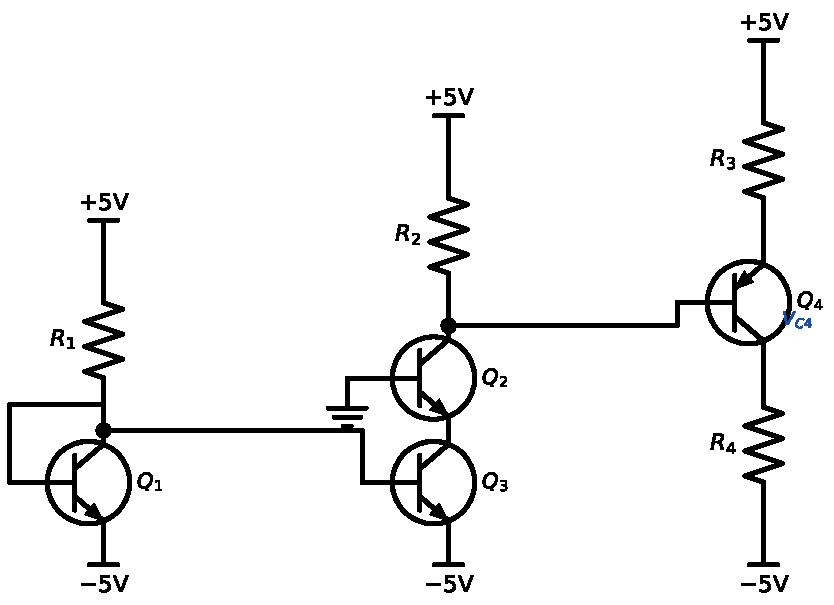
\includegraphics[width=0.9\linewidth,height=6cm,keepaspectratio]{p17_circuit}\end{center}
\solstep{1}{Rules}With $I_B\approx0$ and every transistor active ($|V_{BE}|=0.7$\,V, $I_C\approx I_E$), a resistor is known as soon as the voltages at both of its ends and the current through it are known: $R = \Delta V / I$. The specifications give the currents and some node voltages; the remaining freedom is removed with two rules:\begin{itemize}[leftmargin=*,itemsep=1pt]
\item $V_{BE}$-insensitive: the voltage across the resistor that sets an emitter current must be at least $1$\,V (then $\pm0.1$\,V of $V_{BE}$ changes $I_C$ by at most $10\,\%$);
\item $\beta$-insensitive: a divider current must be much larger ($\ge 10\times$) than the base current it feeds, and a collector current that drives a base must be much larger than that base current.
\end{itemize}
Work from the nodes that are already fixed towards the unknown ones.
\solstep{2}{Design, node by node}\begin{enumerate}[leftmargin=*,itemsep=3pt]
\item $V_{BE}$-insensitivity: a $0.1$\,V change of $V_{BE}$ changes the voltage across $R_{3}$ by $0.1$\,V, so $\frac{\Delta I_C}{I_C} = \frac{0.1}{V_{R3}} \le 10\%$ needs $V_{R3} \ge 1$\,V. Choose the smallest value, $V_{R3} = 1$\,V: $V_{E4} = 5 - V_{R3} = 5 - 1 = 4\,\mathrm{V}$.
\item $Q_{1}$ (diode-connected) is active: $V_{B1} = (-5) + 0.7 = -4.3\,\mathrm{V}$.
\item $Q_{2}$ is active: $V_{E2} = 0 - 0.7 = -0.7\,\mathrm{V}$.
\item $Q_{4}$ is active: $V_{C2} = V_{E4} - 0.7 = 3.3\,\mathrm{V}$.
\item $Q_{3}$ mirrors $Q_{1}$ (same base and emitter nodes): $I_{C3} = I_{C1} = 1\,\mathrm{m}\mathrm{A}$.
\item KCL at $V_{E2}$ ($I_B\approx0$): $I_{E2} = I_{C3} = 1\,\mathrm{m}\mathrm{A}$ $\approx I_{C2}$.
\item With $I_B\approx0$ the only current through $R_{1}$ is $I_{C1}$: $I_{R1} = I_{C1} = 1\,\mathrm{m}\mathrm{A}$.
\item $\displaystyle R_{1} = \frac{5 - V_{B1}}{I_{C1}} = \frac{5 - (-4.3)}{1\,\mathrm{m}\mathrm{A}} = \mathbf{9.3\,\mathrm{k}\Omega}$
\item With $I_B\approx0$ the only current through $R_{2}$ is $I_{C2}$: $I_{R2} = I_{C2} = 1\,\mathrm{m}\mathrm{A}$.
\item $\displaystyle R_{2} = \frac{5 - V_{C2}}{I_{C2}} = \frac{5 - 3.3}{1\,\mathrm{m}\mathrm{A}} = \mathbf{1.7\,\mathrm{k}\Omega}$
\item With $I_B\approx0$ the only current through $R_{3}$ is $I_{E4}$: $I_{R3} = I_{E4} = 2\,\mathrm{m}\mathrm{A}$ ($I_C\approx I_E$).
\item $\displaystyle R_{3} = \frac{5 - V_{E4}}{I_{E4}} = \frac{5 - 4}{2\,\mathrm{m}\mathrm{A}} = \mathbf{500\,\Omega}$
\item With $I_B\approx0$ the only current through $R_{4}$ is $I_{C4}$: $I_{R4} = I_{C4} = 2\,\mathrm{m}\mathrm{A}$.
\item $\displaystyle R_{4} = \frac{V_{C4} - (-5)}{I_{C4}} = \frac{-1 - (-5)}{2\,\mathrm{m}\mathrm{A}} = \mathbf{2\,\mathrm{k}\Omega}$
\end{enumerate}

\solstep{3}{Designed circuit}\begin{center}\renewcommand{\arraystretch}{1.35}
\begin{tabular}{cc}
\toprule
resistor & value \\
\midrule
$R_{1}$ & $9.3\,\mathrm{k}\Omega$ \\
$R_{2}$ & $1.7\,\mathrm{k}\Omega$ \\
$R_{3}$ & $500\,\Omega$ \\
$R_{4}$ & $2\,\mathrm{k}\Omega$ \\
\bottomrule
\end{tabular}\end{center}
\begin{center}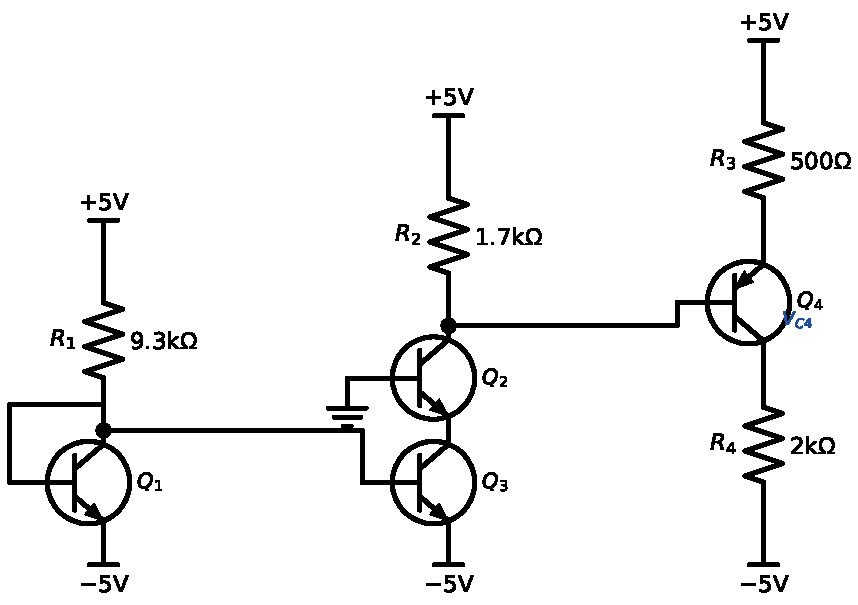
\includegraphics[width=0.85\linewidth,height=6cm,keepaspectratio]{p17_designed}\end{center}

\solstep{4}{Check the design}\begin{itemize}[leftmargin=*,itemsep=2pt]
\item $I_{B1} = \frac{I_{C1}}{\beta} = 10\,\mu \mathrm{A}$ (all bases on this node: $20\,\mu \mathrm{A}$) $\ll$ the $1\,\mathrm{m}\mathrm{A}$ flowing in the base network \checkmark
\item $I_{B3} = \frac{I_{C3}}{\beta} = 10\,\mu \mathrm{A}$ (all bases on this node: $20\,\mu \mathrm{A}$) $\ll$ the $1\,\mathrm{m}\mathrm{A}$ flowing in the base network \checkmark
\item $I_{B4} = \frac{I_{C4}}{\beta} = 20\,\mu \mathrm{A}$ $\ll$ the $1\,\mathrm{m}\mathrm{A}$ flowing in the base network \checkmark
\item $Q_{1}$ is diode-connected: $V_{CE1} = |V_{BE}| = 0.7$\,V, always active (the $|V_{CE}|$ specification is meant for the other transistors) \checkmark
\item $V_{CE2} = V_{C2} - V_{E2} = 3.3 - (-0.7) = 4\,\mathrm{V} \ge 1$\,V \checkmark
\item $V_{CE3} = V_{E2} - (-5) = -0.7 - (-5) = 4.3\,\mathrm{V} \ge 1$\,V \checkmark
\item $V_{EC4} = V_{E4} - V_{C4} = 4 - (-1) = 5\,\mathrm{V} \ge 1$\,V \checkmark
\end{itemize}
Finally the designed circuit is solved exactly ($\beta=100$, base currents included), once with $|V_{BE}|=0.7$\,V and once with each transistor's $|V_{BE}|$ changed to $0.6$ and $0.8$\,V:\begin{center}\renewcommand{\arraystretch}{1.35}
\begin{tabular}{cccccc}
\toprule
 & target $I_C$ & exact $I_C$ & $|V_{BE}|=0.6$ & $|V_{BE}|=0.8$ & max change \\
\midrule
$Q_{1}$ & $1\,\mathrm{m}\mathrm{A}$ & $980\,\mu \mathrm{A}$ & $991\,\mu \mathrm{A}$ & $970\,\mu \mathrm{A}$ & $1.1\,\%$ \\
$Q_{2}$ & $1\,\mathrm{m}\mathrm{A}$ & $971\,\mu \mathrm{A}$ & $971\,\mu \mathrm{A}$ & $971\,\mu \mathrm{A}$ & $0\,\%$ \\
$Q_{3}$ & $1\,\mathrm{m}\mathrm{A}$ & $980\,\mu \mathrm{A}$ & $991\,\mu \mathrm{A}$ & $970\,\mu \mathrm{A}$ & $1.1\,\%$ \\
$Q_{4}$ & $2\,\mathrm{m}\mathrm{A}$ & $1.82\,\mathrm{m}\mathrm{A}$ & $2.01\,\mathrm{m}\mathrm{A}$ & $1.63\,\mathrm{m}\mathrm{A}$ & $9.6\,\%$ \\
\bottomrule
\end{tabular}\end{center}
A $\pm0.1$\,V change of $V_{BE}$ moves no current by more than about $10\,\%$ of its design value ($V_{BE}$-insensitive), and the exact currents are close to the targets ($I_B$ negligible). The exact currents drift further from the targets along a chain of direct-coupled stages: each base current and each $I_C = \alpha I_E$ slightly shifts the collector voltage that biases the next stage, and with only $\approx1$\,V across the next emitter resistor that shift is amplified. This is the normal accuracy of a hand design with $I_B\approx0$; a larger emitter-resistor voltage in the later stages reduces the drift.
\begin{ansbox}
$R_{1} = 9.3\,\mathrm{k}\Omega$,\quad $R_{2} = 1.7\,\mathrm{k}\Omega$,\quad $R_{3} = 500\,\Omega$,\quad $R_{4} = 2\,\mathrm{k}\Omega$
\end{ansbox}

\newpage
\subsection*{Solution 4C.18 \hfill Hard}
\begin{center}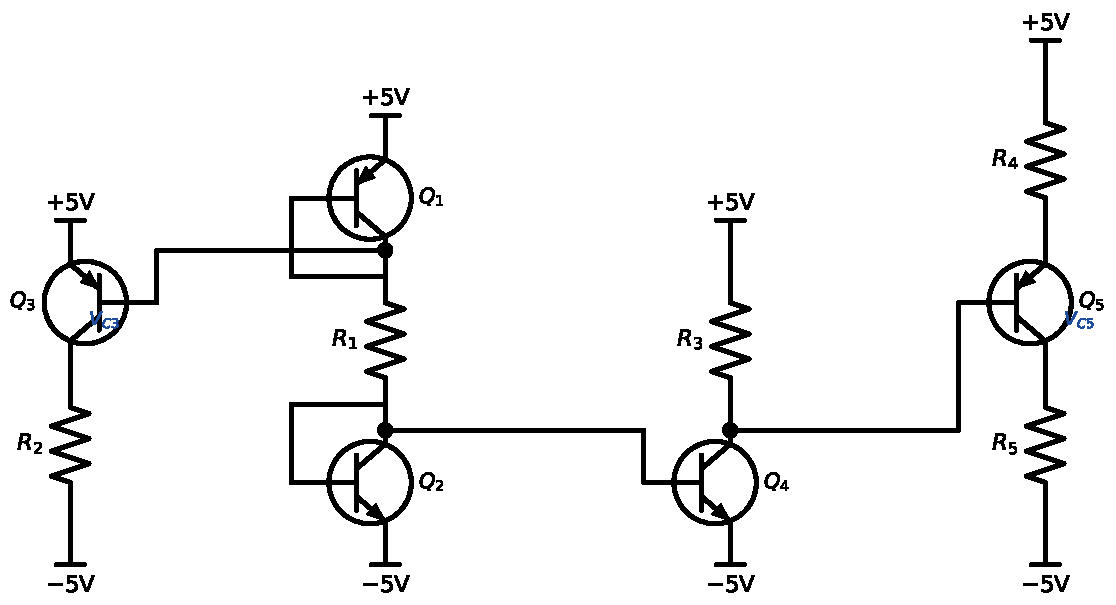
\includegraphics[width=0.9\linewidth,height=6cm,keepaspectratio]{p18_circuit}\end{center}
\solstep{1}{Rules}With $I_B\approx0$ and every transistor active ($|V_{BE}|=0.7$\,V, $I_C\approx I_E$), a resistor is known as soon as the voltages at both of its ends and the current through it are known: $R = \Delta V / I$. The specifications give the currents and some node voltages; the remaining freedom is removed with two rules:\begin{itemize}[leftmargin=*,itemsep=1pt]
\item $V_{BE}$-insensitive: the voltage across the resistor that sets an emitter current must be at least $1$\,V (then $\pm0.1$\,V of $V_{BE}$ changes $I_C$ by at most $10\,\%$);
\item $\beta$-insensitive: a divider current must be much larger ($\ge 10\times$) than the base current it feeds, and a collector current that drives a base must be much larger than that base current.
\end{itemize}
Work from the nodes that are already fixed towards the unknown ones.
\solstep{2}{Design, node by node}\begin{enumerate}[leftmargin=*,itemsep=3pt]
\item $V_{BE}$-insensitivity: a $0.1$\,V change of $V_{BE}$ changes the voltage across $R_{4}$ by $0.1$\,V, so $\frac{\Delta I_C}{I_C} = \frac{0.1}{V_{R4}} \le 10\%$ needs $V_{R4} \ge 1$\,V. Choose the smallest value, $V_{R4} = 1$\,V: $V_{E5} = 5 - V_{R4} = 5 - 1 = 4\,\mathrm{V}$.
\item $Q_{3}$ is active: $V_{B3} = 5 - 0.7 = 4.3\,\mathrm{V}$.
\item $Q_{2}$ (diode-connected) is active: $V_{B2} = (-5) + 0.7 = -4.3\,\mathrm{V}$.
\item $Q_{5}$ is active: $V_{C4} = V_{E5} - 0.7 = 3.3\,\mathrm{V}$.
\item $Q_{3}$ mirrors $Q_{1}$ (same base and emitter nodes): $I_{C3} = I_{C1} = 1\,\mathrm{m}\mathrm{A}$.
\item With $I_B\approx0$ the only current through $R_{2}$ is $I_{C3}$: $I_{R2} = I_{C3} = 1\,\mathrm{m}\mathrm{A}$.
\item $\displaystyle R_{2} = \frac{V_{C3} - (-5)}{I_{C3}} = \frac{2 - (-5)}{1\,\mathrm{m}\mathrm{A}} = \mathbf{7\,\mathrm{k}\Omega}$
\item With $I_B\approx0$ the only current through $R_{1}$ is $I_{C1}$: $I_{R1} = I_{C1} = 1\,\mathrm{m}\mathrm{A}$.
\item $\displaystyle R_{1} = \frac{V_{B3} - V_{B2}}{I_{C1}} = \frac{4.3 - (-4.3)}{1\,\mathrm{m}\mathrm{A}} = \mathbf{8.6\,\mathrm{k}\Omega}$
\item KCL at $V_{B2}$ ($I_B\approx0$): $I_{C2} = I_{C1} = 1\,\mathrm{m}\mathrm{A}$.
\item $Q_{4}$ mirrors $Q_{2}$ (same base and emitter nodes): $I_{C4} = I_{C2} = 1\,\mathrm{m}\mathrm{A}$.
\item With $I_B\approx0$ the only current through $R_{3}$ is $I_{C4}$: $I_{R3} = I_{C4} = 1\,\mathrm{m}\mathrm{A}$.
\item $\displaystyle R_{3} = \frac{5 - V_{C4}}{I_{C4}} = \frac{5 - 3.3}{1\,\mathrm{m}\mathrm{A}} = \mathbf{1.7\,\mathrm{k}\Omega}$
\item With $I_B\approx0$ the only current through $R_{4}$ is $I_{E5}$: $I_{R4} = I_{E5} = 2\,\mathrm{m}\mathrm{A}$ ($I_C\approx I_E$).
\item $\displaystyle R_{4} = \frac{5 - V_{E5}}{I_{E5}} = \frac{5 - 4}{2\,\mathrm{m}\mathrm{A}} = \mathbf{500\,\Omega}$
\item With $I_B\approx0$ the only current through $R_{5}$ is $I_{C5}$: $I_{R5} = I_{C5} = 2\,\mathrm{m}\mathrm{A}$.
\item $\displaystyle R_{5} = \frac{V_{C5} - (-5)}{I_{C5}} = \frac{-2 - (-5)}{2\,\mathrm{m}\mathrm{A}} = \mathbf{1.5\,\mathrm{k}\Omega}$
\end{enumerate}

\solstep{3}{Designed circuit}\begin{center}\renewcommand{\arraystretch}{1.35}
\begin{tabular}{cc}
\toprule
resistor & value \\
\midrule
$R_{1}$ & $8.6\,\mathrm{k}\Omega$ \\
$R_{2}$ & $7\,\mathrm{k}\Omega$ \\
$R_{3}$ & $1.7\,\mathrm{k}\Omega$ \\
$R_{4}$ & $500\,\Omega$ \\
$R_{5}$ & $1.5\,\mathrm{k}\Omega$ \\
\bottomrule
\end{tabular}\end{center}
\begin{center}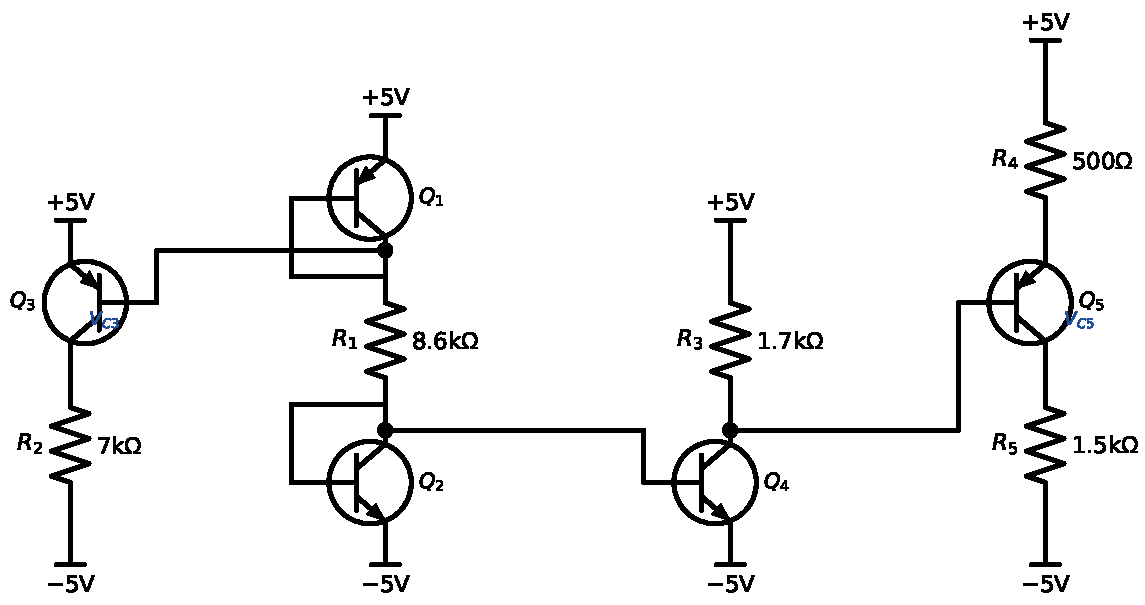
\includegraphics[width=0.85\linewidth,height=6cm,keepaspectratio]{p18_designed}\end{center}

\solstep{4}{Check the design}\begin{itemize}[leftmargin=*,itemsep=2pt]
\item $I_{B3} = \frac{I_{C3}}{\beta} = 10\,\mu \mathrm{A}$ (all bases on this node: $20\,\mu \mathrm{A}$) $\ll$ the $1\,\mathrm{m}\mathrm{A}$ flowing in the base network \checkmark
\item $I_{B1} = \frac{I_{C1}}{\beta} = 10\,\mu \mathrm{A}$ (all bases on this node: $20\,\mu \mathrm{A}$) $\ll$ the $1\,\mathrm{m}\mathrm{A}$ flowing in the base network \checkmark
\item $I_{B2} = \frac{I_{C2}}{\beta} = 10\,\mu \mathrm{A}$ (all bases on this node: $20\,\mu \mathrm{A}$) $\ll$ the $1\,\mathrm{m}\mathrm{A}$ flowing in the base network \checkmark
\item $I_{B4} = \frac{I_{C4}}{\beta} = 10\,\mu \mathrm{A}$ (all bases on this node: $20\,\mu \mathrm{A}$) $\ll$ the $1\,\mathrm{m}\mathrm{A}$ flowing in the base network \checkmark
\item $I_{B5} = \frac{I_{C5}}{\beta} = 20\,\mu \mathrm{A}$ $\ll$ the $1\,\mathrm{m}\mathrm{A}$ flowing in the base network \checkmark
\item $V_{EC3} = 5 - V_{C3} = 5 - 2 = 3\,\mathrm{V} \ge 1$\,V \checkmark
\item $Q_{1}$ is diode-connected: $V_{EC1} = |V_{BE}| = 0.7$\,V, always active (the $|V_{CE}|$ specification is meant for the other transistors) \checkmark
\item $Q_{2}$ is diode-connected: $V_{CE2} = |V_{BE}| = 0.7$\,V, always active (the $|V_{CE}|$ specification is meant for the other transistors) \checkmark
\item $V_{CE4} = V_{C4} - (-5) = 3.3 - (-5) = 8.3\,\mathrm{V} \ge 1$\,V \checkmark
\item $V_{EC5} = V_{E5} - V_{C5} = 4 - (-2) = 6\,\mathrm{V} \ge 1$\,V \checkmark
\end{itemize}
Finally the designed circuit is solved exactly ($\beta=100$, base currents included), once with $|V_{BE}|=0.7$\,V and once with each transistor's $|V_{BE}|$ changed to $0.6$ and $0.8$\,V:\begin{center}\renewcommand{\arraystretch}{1.35}
\begin{tabular}{cccccc}
\toprule
 & target $I_C$ & exact $I_C$ & $|V_{BE}|=0.6$ & $|V_{BE}|=0.8$ & max change \\
\midrule
$Q_{3}$ & $1\,\mathrm{m}\mathrm{A}$ & $980\,\mu \mathrm{A}$ & $992\,\mu \mathrm{A}$ & $969\,\mu \mathrm{A}$ & $1.1\,\%$ \\
$Q_{1}$ & $1\,\mathrm{m}\mathrm{A}$ & $980\,\mu \mathrm{A}$ & $992\,\mu \mathrm{A}$ & $969\,\mu \mathrm{A}$ & $1.1\,\%$ \\
$Q_{2}$ & $1\,\mathrm{m}\mathrm{A}$ & $980\,\mu \mathrm{A}$ & $992\,\mu \mathrm{A}$ & $969\,\mu \mathrm{A}$ & $1.1\,\%$ \\
$Q_{4}$ & $1\,\mathrm{m}\mathrm{A}$ & $980\,\mu \mathrm{A}$ & $992\,\mu \mathrm{A}$ & $969\,\mu \mathrm{A}$ & $1.1\,\%$ \\
$Q_{5}$ & $2\,\mathrm{m}\mathrm{A}$ & $1.85\,\mathrm{m}\mathrm{A}$ & $2.04\,\mathrm{m}\mathrm{A}$ & $1.66\,\mathrm{m}\mathrm{A}$ & $9.6\,\%$ \\
\bottomrule
\end{tabular}\end{center}
A $\pm0.1$\,V change of $V_{BE}$ moves no current by more than about $10\,\%$ of its design value ($V_{BE}$-insensitive), and the exact currents are close to the targets ($I_B$ negligible). The exact currents drift further from the targets along a chain of direct-coupled stages: each base current and each $I_C = \alpha I_E$ slightly shifts the collector voltage that biases the next stage, and with only $\approx1$\,V across the next emitter resistor that shift is amplified. This is the normal accuracy of a hand design with $I_B\approx0$; a larger emitter-resistor voltage in the later stages reduces the drift.
\begin{ansbox}
$R_{1} = 8.6\,\mathrm{k}\Omega$,\quad $R_{2} = 7\,\mathrm{k}\Omega$,\quad $R_{3} = 1.7\,\mathrm{k}\Omega$,\quad $R_{4} = 500\,\Omega$,\quad $R_{5} = 1.5\,\mathrm{k}\Omega$
\end{ansbox}

\end{document}
